\documentclass[aos]{imsart}
\startlocaldefs
\RequirePackage{amsthm,amsmath,amsfonts,amssymb,mathtools}
\RequirePackage[authoryear]{natbib}
\RequirePackage{graphicx,booktabs,array}
\RequirePackage{enumitem}
\RequirePackage{xcolor}
\RequirePackage{algorithm}
\RequirePackage{algpseudocode}
\RequirePackage[colorlinks,citecolor=blue!50!black,urlcolor=blue!50!black,linkcolor=blue!50!black]{hyperref}

\numberwithin{equation}{section}
\theoremstyle{plain}
\newtheorem{theorem}{Theorem}[section]
\newtheorem{proposition}[theorem]{Proposition}
\newtheorem{lemma}[theorem]{Lemma}
\newtheorem{corollary}[theorem]{Corollary}
\theoremstyle{definition}
\newtheorem{definition}[theorem]{Definition}
\newtheorem{assumption}[theorem]{Assumption}
\newtheorem{example}[theorem]{Example}
\newtheorem{remark}[theorem]{Remark}

\renewcommand{\topfraction}{0.85}
\renewcommand{\bottomfraction}{0.6}
\renewcommand{\textfraction}{0.1}
\renewcommand{\floatpagefraction}{0.75}
\setlength{\emergencystretch}{3em}
\newcommand{\fittable}[1]{\begingroup\footnotesize\setlength{\tabcolsep}{4pt}\input{#1}\endgroup}

\newcommand{\rev}[1]{#1}
\newenvironment{revblock}{}{}
\newcommand{\rp}{\psi}

\newcommand{\Pp}{\mathbb{P}}
\newcommand{\E}{\mathbb{E}}
\newcommand{\Hh}{\mathcal{H}}
\newcommand{\R}{\mathbb{R}}
\newcommand{\MMD}{\operatorname{MMD}}
\newcommand{\TV}{d_{\mathrm{TV}}}
\DeclareMathOperator*{\argmin}{arg\,min}
\newcommand{\dist}{\operatorname{dist}}
\newcommand{\supp}{\operatorname{supp}}
\newcommand{\diam}{\operatorname{diam}}
\newcommand{\BlackBox}{\qed}

% Generated by trimmedmmd.experiments.realdata_run -- do not edit.
\newcommand{\rhcDzero}{0.111}
\newcommand{\rhcTauzero}{0.074}
\newcommand{\rhcGap}{0.7}
\newcommand{\rhcScreen}{0.143}
\newcommand{\rhcAhat}{0.05}
\newcommand{\rhcLast}{0.00}
\newcommand{\rhcNeed}{1{,}205}
\newcommand{\rhcN}{2{,}184}
\newcommand{\rhcM}{3{,}551}
\newcommand{\rhcLo}{0.30}
\newcommand{\rhcLoMin}{0.30}
\newcommand{\rhcLoMax}{0.30}
\newcommand{\rhcCertN}{8}
\newcommand{\nhaneschildDzero}{0.406}
\newcommand{\nhaneschildTauzero}{0.084}
\newcommand{\nhaneschildGap}{0.2}
\newcommand{\nhaneschildScreen}{0.162}
\newcommand{\nhaneschildAhat}{0.45}
\newcommand{\nhaneschildLast}{0.40}
\newcommand{\nhaneschildNeed}{91}
\newcommand{\nhaneschildN}{1{,}969}
\newcommand{\nhaneschildM}{2{,}300}
\newcommand{\nhaneschildLo}{0.75}
\newcommand{\nhaneschildLoMin}{0.75}
\newcommand{\nhaneschildLoMax}{0.75}
\newcommand{\nhaneschildCertN}{8}
\newcommand{\nhanesageDzero}{0.220}
\newcommand{\nhanesageTauzero}{0.079}
\newcommand{\nhanesageGap}{0.4}
\newcommand{\nhanesageScreen}{0.152}
\newcommand{\nhanesageAhat}{0.15}
\newcommand{\nhanesageLast}{0.10}
\newcommand{\nhanesageNeed}{310}
\newcommand{\nhanesageN}{2{,}519}
\newcommand{\nhanesageM}{2{,}300}
\newcommand{\nhanesageLo}{0.35}
\newcommand{\nhanesageLoMin}{0.35}
\newcommand{\nhanesageLoMax}{0.35}
\newcommand{\nhanesageCertN}{8}
\newcommand{\nhanesbmiDzero}{0.069}
\newcommand{\nhanesbmiTauzero}{0.091}
\newcommand{\nhanesbmiGap}{1.3}
\newcommand{\nhanesbmiScreen}{0.176}
\newcommand{\nhanesbmiAhat}{0.00}
\newcommand{\nhanesbmiLast}{0.00}
\newcommand{\nhanesbmiNeed}{3{,}120}
\newcommand{\nhanesbmiN}{1{,}627}
\newcommand{\nhanesbmiM}{2{,}008}
\newcommand{\nhanesbmiLo}{0.05}
\newcommand{\nhanesbmiLoMin}{0.00}
\newcommand{\nhanesbmiLoMax}{0.10}
\newcommand{\nhanesbmiCertN}{7}
\newcommand{\rhcSharpHalf}{13{,}810}
\newcommand{\rhcSharpHalfAlpha}{0.15}
\newcommand{\rhcSharpFourFifths}{91{,}881}
\newcommand{\rhcSharpFourFifthsAlpha}{0.25}
\newcommand{\nhaneschildSharpHalf}{1{,}725}
\newcommand{\nhaneschildSharpHalfAlpha}{0.40}
\newcommand{\nhaneschildSharpFourFifths}{9{,}509}
\newcommand{\nhaneschildSharpFourFifthsAlpha}{0.60}
\newcommand{\nhanesageSharpHalf}{3{,}373}
\newcommand{\nhanesageSharpHalfAlpha}{0.15}
\newcommand{\nhanesageSharpFourFifths}{75{,}009}
\newcommand{\nhanesageSharpFourFifthsAlpha}{0.30}
\newcommand{\nhanesbmiSharpFourFifths}{24{,}444}
\newcommand{\nhanesbmiSharpFourFifthsAlpha}{0.05}
\newcommand{\sharpFourFifthsLo}{9{,}509}
\newcommand{\sharpFourFifthsHi}{91{,}881}
\newcommand{\rhcCrumpCut}{0.106}
\newcommand{\rhcCrumpDrop}{0.10}
\newcommand{\rhcRuleDrop}{0.09}

% Generated by trimmedmmd.experiments.trimmings_run -- do not edit.
\newcommand{\trimFracBelow}{2}
\newcommand{\trimFracAbove}{379}
\newcommand{\trimFracShareAbove}{1.00}
\newcommand{\trimWFracBelow}{0}
\newcommand{\trimRecall}{0.87}
\newcommand{\trimWRecall}{0.97}
\newcommand{\trimJaccard}{0.75}
\newcommand{\trimAlphaStar}{0.10}
\newcommand{\trimBudgetAbove}{0.48}
\newcommand{\trimJacTwoBelow}{0.97}
\newcommand{\trimJacTwoAbove}{0.88}
\newcommand{\trimValGapAbove}{2.3e-06}

% Generated by trimmedmmd.experiments.realdata_run -- do not edit.
\newcommand{\cohAlpha}{0.30}
\newcommand{\cohKeptX}{1{,}565}
\newcommand{\cohKeptY}{2{,}520}
\newcommand{\cohNX}{2{,}184}
\newcommand{\cohNY}{3{,}551}
\newcommand{\cohSmdBefore}{0.50}
\newcommand{\cohSmdAfter}{0.04}
\newcommand{\cohSmdMeanBefore}{0.16}
\newcommand{\cohSmdMeanAfter}{0.01}
\newcommand{\cohFracX}{70}
\newcommand{\cohEssX}{1541}
\newcommand{\cohIdentified}{no}
\newcommand{\cohDhat}{0.013}
\newcommand{\cohTau}{0.148}
\newcommand{\cohWSmdBefore}{0.49}
\newcommand{\cohWSmdAfter}{0.34}
\newcommand{\cohWN}{1{,}400}
\newcommand{\cohWFracX}{0}
\newcommand{\cohNhAlpha}{0.75}
\newcommand{\cohNhKeptX}{501}
\newcommand{\cohNhKeptY}{590}
\newcommand{\cohPropBefore}{0.62}
\newcommand{\cohPropAfter}{0.83}
\newcommand{\cohWorstCov}{\texttt{aps1}}
\newcommand{\cohWorstBefore}{0.50}
\newcommand{\cohWorstAfter}{0.02}

% Generated by scripts/perm.py -- do not edit.
\newcommand{\permB}{200}
\newcommand{\permMax}{0.022}
\newcommand{\permQ}{0.020}
\newcommand{\permP}{0.005}
\newcommand{\permMMD}{0.111}

% Generated by scripts/fig2.py -- do not edit.
\newcommand{\rgSep}{3}
\newcommand{\rgLevels}{0.15, 0.2, 0.3, 0.4}
\newcommand{\rgNmin}{100}
\newcommand{\rgNmax}{16{,}000}
\newcommand{\rgReps}{455}
\newcommand{\rgDzeroPerA}{1.00}
\newcommand{\rgCoverMiss}{0}
\newcommand{\rgDelta}{0.05}
\newcommand{\rgFireOneFive}{663}
\newcommand{\rgHalfOneFive}{5{,}215}
\newcommand{\rgSharpOneFive}{160{,}470}
\newcommand{\rgAhatOneFive}{0.100}
\newcommand{\rgCertOneFive}{0.125}
\newcommand{\rgCertOneSplitOneFive}{0.133}
\newcommand{\rgCertBootOneFive}{0.133}
\newcommand{\rgNatOneFive}{16{,}000}
\newcommand{\rgRecallOneFive}{0.98}
\newcommand{\rgFireTwoZero}{373}
\newcommand{\rgHalfTwoZero}{3{,}248}
\newcommand{\rgSharpTwoZero}{103{,}767}
\newcommand{\rgAhatTwoZero}{0.150}
\newcommand{\rgCertTwoZero}{0.183}
\newcommand{\rgCertOneSplitTwoZero}{0.183}
\newcommand{\rgCertBootTwoZero}{0.175}
\newcommand{\rgNatTwoZero}{16{,}000}
\newcommand{\rgRecallTwoZero}{0.97}
\newcommand{\rgFireThreeZero}{166}
\newcommand{\rgHalfThreeZero}{1{,}716}
\newcommand{\rgSharpThreeZero}{59{,}266}
\newcommand{\rgAhatThreeZero}{0.250}
\newcommand{\rgCertThreeZero}{0.275}
\newcommand{\rgCertOneSplitThreeZero}{0.275}
\newcommand{\rgCertBootThreeZero}{0.275}
\newcommand{\rgNatThreeZero}{16{,}000}
\newcommand{\rgRecallThreeZero}{0.98}
\newcommand{\rgFireFourZero}{93}
\newcommand{\rgHalfFourZero}{1{,}125}
\newcommand{\rgSharpFourZero}{42{,}135}
\newcommand{\rgAhatFourZero}{0.342}
\newcommand{\rgCertFourZero}{0.375}
\newcommand{\rgCertOneSplitFourZero}{0.383}
\newcommand{\rgCertBootFourZero}{0.383}
\newcommand{\rgNatFourZero}{16{,}000}
\newcommand{\rgRecallFourZero}{0.99}
\newcommand{\rgCertRecoverLo}{83}
\newcommand{\rgCertRecoverHi}{94}
\newcommand{\rgAnaRecoverLo}{67}
\newcommand{\rgAnaRecoverHi}{85}

% Generated by scripts/fair_macros.py -- do not edit.
\newcommand{\fairAdN}{30{,}527}
\newcommand{\fairAdM}{14{,}695}
\newcommand{\fairAdD}{12}
\newcommand{\fairAdAhat}{0.350}
\newcommand{\fairAdLast}{0.25}
\newcommand{\fairAdSplit}{0.40}
\newcommand{\fairAdClf}{0.496}
\newcommand{\fairAdRateM}{0.312}
\newcommand{\fairAdRateW}{0.114}
\newcommand{\fairAdDp}{0.184}
\newcommand{\fairAdSmd}{0.91}
\newcommand{\fairAdRead}{0.50}
\newcommand{\fairAdFloor}{0.00}
\newcommand{\fairAdKernTv}{0.113}
\newcommand{\fairAdKernEss}{0.61}
\newcommand{\fairAdKernDp}{0.002}
\newcommand{\fairAdKernGap}{0.002}
\newcommand{\fairAdKernSmd}{0.00}
\newcommand{\fairAdGbmTv}{0.233}
\newcommand{\fairAdLogitTv}{0.408}
\newcommand{\fairAdAhatTv}{0.382}
\newcommand{\fairAcsN}{62{,}543}
\newcommand{\fairAcsM}{57{,}457}
\newcommand{\fairAcsD}{15}
\newcommand{\fairAcsAhat}{0.250}
\newcommand{\fairAcsLast}{0.20}
\newcommand{\fairAcsSplit}{0.30}
\newcommand{\fairAcsClf}{0.380}
\newcommand{\fairAcsRateM}{0.439}
\newcommand{\fairAcsRateW}{0.289}
\newcommand{\fairAcsDp}{0.073}
\newcommand{\fairAcsSmd}{0.51}
\newcommand{\fairAcsRead}{0.35}
\newcommand{\fairAcsFloor}{0.05}
\newcommand{\fairAcsKernTv}{0.139}
\newcommand{\fairAcsKernEss}{0.73}
\newcommand{\fairAcsKernDp}{0.017}
\newcommand{\fairAcsKernGap}{0.122}
\newcommand{\fairAcsKernSmd}{0.00}
\newcommand{\fairAcsGbmTv}{0.193}
\newcommand{\fairAcsLogitTv}{0.349}
\newcommand{\fairAcsAhatTv}{0.277}
\newcommand{\fairRulesLo}{0.36}
\newcommand{\fairRulesHi}{0.44}
\newcommand{\fairBwUnion}{0.273}
\newcommand{\fairBwUnionScale}{0.7}
\newcommand{\fairBwTune}{0.284}
\newcommand{\fairBwTuneScale}{0.7}
\newcommand{\fairBwK}{7}
\newcommand{\eNineteenNullViol}{0.00}
\newcommand{\slackLo}{7}
\newcommand{\slackHi}{14}

% Generated by scripts/fig_regions.py -- do not edit.
\newcommand{\regTV}{0.45}
\newcommand{\regAlphaLo}{0.20}
\newcommand{\regAlphaHi}{0.65}

% Generated by scripts/probe_trimming.py summarize -- do not edit.
\newcommand{\probeTrimSlope}{-0.49}
\newcommand{\probeTrimSlopeLo}{-0.52}
\newcommand{\probeTrimSlopeHi}{-0.45}
\newcommand{\probeTrimMedFirst}{0.036}
\newcommand{\probeTrimMedLast}{0.006}
\newcommand{\probeTrimNFirst}{250}
\newcommand{\probeTrimNLast}{8{,}000}
\newcommand{\probeWitRatioMax}{0.07}
\newcommand{\probeWitSlope}{-0.50}
\newcommand{\probeReps}{200}
\newcommand{\probeSolverErr}{4e-6}

% Generated by jmlr/tools/make_tables.py; do not edit by hand.
\newcommand{\splitReps}{200}
\newcommand{\splitLowA}{0.108}
\newcommand{\splitUpA}{0.321}
\newcommand{\splitCovMin}{0.99}
\newcommand{\splitCovMax}{1.00}
\newcommand{\splitWidthRootA}{3.01}
\newcommand{\splitWidthRootB}{3.22}
\newcommand{\splitWidthRootC}{3.30}
\newcommand{\splitWidthRootMean}{3.18}
\newcommand{\splitWindowN}{6{,}300}
\newcommand{\calibReps}{400}
\newcommand{\calibRatio}{13}
\newcommand{\calibRatioNew}{5.1}
\newcommand{\costNFactorLo}{26}
\newcommand{\costNFactorHi}{200}
\newcommand{\costRatioHi}{14}
\newcommand{\rgContamReps}{392}
\newcommand{\rgCertBoundary}{12}
\newcommand{\rgCertBoundaryPct}{3.1}
\newcommand{\rgCertOver}{2}
\newcommand{\rgCertBootBoundaryPct}{4.3}
\newcommand{\rgRepsMin}{3}
\newcommand{\rgRepsMax}{20}
\newcommand{\rhcPathSeconds}{200}
\newcommand{\realdataMinutes}{55.7}
\newcommand{\realdataCPUs}{48}
\newcommand{\rhcRatioCrump}{3.1}
\newcommand{\rhcRatioRule}{3.4}
\newcommand{\cZeroDisjoint}{1.47}
\newcommand{\cZeroGaussA}{0.97}
\newcommand{\cZeroGaussB}{0.72}
\newcommand{\cZeroGaussC}{0.43}
\newcommand{\cZeroGaussD}{0.33}
\newcommand{\clfPowA}{0.70}
\newcommand{\clfTypeIA}{0.02}
\newcommand{\clfPowB}{0.95}
\newcommand{\clfTypeIB}{0.02}
\newcommand{\clfPowC}{1.00}
\newcommand{\clfTypeIC}{0.01}
\newcommand{\clfPowD}{1.00}
\newcommand{\clfTypeID}{0.08}
\newcommand{\clfPowE}{1.00}
\newcommand{\clfTypeIE}{0.03}
\newcommand{\clfReps}{100}
\newcommand{\vbNhPilotAhat}{0.45}
\newcommand{\vbNhPilotLast}{0.40}
\newcommand{\vbNhUnionAhat}{0.45}
\newcommand{\vbNhUnionLast}{0.40}
\newcommand{\vbNhStrictAhat}{0.40}
\newcommand{\vbNhStrictLast}{0.35}
\newcommand{\vbAcsPilotAhat}{0.25}
\newcommand{\vbAcsPilotLast}{0.20}
\newcommand{\vbAcsUnionAhat}{0.25}
\newcommand{\vbAcsUnionLast}{0.20}
\newcommand{\vbAcsStrictAhat}{0.20}
\newcommand{\vbAcsStrictLast}{0.15}
\newcommand{\vbNhPilotN}{1{,}379}
\newcommand{\vbNhPilotM}{1{,}610}
\newcommand{\balEnergyMaxSmd}{0.013}
\newcommand{\balEnergyMeanSmd}{0.004}
\newcommand{\balEnergyEssX}{0.54}
\newcommand{\balEnergyEssY}{0.78}
\newcommand{\balKernelMaxSmd}{0.014}
\newcommand{\balKernelMeanSmd}{0.004}
\newcommand{\balKernelEssX}{0.27}
\newcommand{\balKernelEssY}{0.44}
\newcommand{\balTrimMaxSmd}{0.041}
\newcommand{\balTrimMeanSmd}{0.011}
\newcommand{\balTrimEssX}{0.71}
\newcommand{\balTrimEssY}{0.70}
\newcommand{\bootLevelHi}{8}
\newcommand{\rhcCertSubLo}{100}
\newcommand{\rhcCertSubHi}{200}

% Generated by jmlr/tools/make_harder_tables.py from results/harder/ (harder synthetic study). Do not edit.
\newcommand{\harderAloGeMaxOne}{0.040}
\newcommand{\harderAloGtMax}{0.035}
\newcommand{\harderAloGtMaxNull}{0.065}
\newcommand{\harderAloNarrowLogit}{0.080}
\newcommand{\harderAloOscBest}{0.396}
\newcommand{\harderAloOscSeq}{0.380}
\newcommand{\harderAloOverlapSixteen}{0.132}
\newcommand{\harderAloSeqMax}{0.114}
\newcommand{\harderAloSeqMin}{0.025}
\newcommand{\harderAloSmallSixteen}{0.018}
\newcommand{\harderAloTauOsc}{0.209}
\newcommand{\harderAloTauOverlap}{0.009}
\newcommand{\harderBMpathLtwo}{0.71}
\newcommand{\harderBetHoefGain}{0.3}
\newcommand{\harderBoundaryBootK}{9}
\newcommand{\harderBoundaryBootRate}{0.045}
\newcommand{\harderBoundaryCells}{73}
\newcommand{\harderBoundaryCellsOne}{71}
\newcommand{\harderBoundaryOthersMax}{0.040}
\newcommand{\harderBoundaryPooledR}{14{,}600}
\newcommand{\harderBoundaryWorstCP}{0.10}
\newcommand{\harderBoundaryWorstFS}{0.065}
\newcommand{\harderBoundaryWorstK}{13}
\newcommand{\harderBoundaryWorstP}{0.20}
\newcommand{\harderBoundaryZeroCP}{0.0002}
\newcommand{\harderBumpHnarrow}{0.307}
\newcommand{\harderBumpHwide}{0.601}
\newcommand{\harderBumpLtwoNarrow}{0.09}
\newcommand{\harderBumpLtwoWide}{0.36}
\newcommand{\harderDmax}{100}
\newcommand{\harderExtCells}{67}
\newcommand{\harderExtDesigns}{17}
\newcommand{\harderExtReplicates}{13{,}400}
\newcommand{\harderExtReps}{200}
\newcommand{\harderFlagK}{19}
\newcommand{\harderFlipBest}{0.11}
\newcommand{\harderFlipEsIters}{21}
\newcommand{\harderFlipEsPowOff}{1.00}
\newcommand{\harderFlipEsPowOn}{0.72}
\newcommand{\harderFlipEsReps}{60}
\newcommand{\harderFlipGbmCap}{0.66}
\newcommand{\harderFlipGbmEight}{0.11}
\newcommand{\harderFlipGbmEighty}{5{,}200}
\newcommand{\harderFlipGbmSixtyFour}{0.90}
\newcommand{\harderFlipKnnEighty}{9{,}100}
\newcommand{\harderGbmBetHoefInf}{67}
\newcommand{\harderGbmBetHoefLoss}{0}
\newcommand{\harderGbmBetHoefMean}{0.30}
\newcommand{\harderGbmBetHoefTie}{5}
\newcommand{\harderGbmBetHoefWin}{62}
\newcommand{\harderGbmSoftHardInf}{69}
\newcommand{\harderGbmSoftHardLoss}{25}
\newcommand{\harderGbmSoftHardMean}{-0.04}
\newcommand{\harderGbmSoftHardTie}{22}
\newcommand{\harderGbmSoftHardWin}{22}
\newcommand{\harderGbmWinsFlip}{1}
\newcommand{\harderGbmWinsNarrow}{2}
\newcommand{\harderGbmWinsOsc}{15}
\newcommand{\harderHalfEightyOscFour}{400}
\newcommand{\harderHalfEightyOscOneMax}{800}
\newcommand{\harderHalfEightyOscOneMin}{100}
\newcommand{\harderHalfEightyOverlap}{800}
\newcommand{\harderHalfLowTVMax}{0.20}
\newcommand{\harderLogitBetHoefInf}{83}
\newcommand{\harderLogitBetHoefLoss}{0}
\newcommand{\harderLogitBetHoefMean}{0.28}
\newcommand{\harderLogitBetHoefTie}{2}
\newcommand{\harderLogitBetHoefWin}{81}
\newcommand{\harderLogitRecheckCP}{0.044}
\newcommand{\harderLogitRecheckDeltaGap}{1\times10^{-7}}
\newcommand{\harderLogitRecheckDeltaMed}{0.1997}
\newcommand{\harderLogitRecheckK}{41}
\newcommand{\harderLogitRecheckNewK}{28}
\newcommand{\harderLogitRecheckNewR}{1{,}000}
\newcommand{\harderLogitRecheckR}{1{,}200}
\newcommand{\harderLogitRecheckRate}{0.034}
\newcommand{\harderLogitSoftHardInf}{83}
\newcommand{\harderLogitSoftHardLoss}{56}
\newcommand{\harderLogitSoftHardMean}{-0.16}
\newcommand{\harderLogitSoftHardTie}{17}
\newcommand{\harderLogitSoftHardWin}{10}
\newcommand{\harderLogitWinsHigh}{4}
\newcommand{\harderLogitWinsNarrow}{6}
\newcommand{\harderLogitWinsOther}{5}
\newcommand{\harderMMDmixed}{0.135}
\newcommand{\harderMMDosc}{0.49}
\newcommand{\harderMMDoscSixteen}{0.019}
\newcommand{\harderMMDoverlap}{0.181}
\newcommand{\harderMMDrestMax}{0.103}
\newcommand{\harderMMDwide}{0.118}
\newcommand{\harderMainReps}{14{,}600}
\newcommand{\harderNcap}{12{,}800}
\newcommand{\harderNdesigns}{18}
\newcommand{\harderNeightyBoth}{15}
\newcommand{\harderNeightyBothSmall}{1}
\newcommand{\harderNeightyRatioMax}{1.3}
\newcommand{\harderNeightyRatioMed}{1.1}
\newcommand{\harderNeightyRatioMin}{1.0}
\newcommand{\harderNmax}{800}
\newcommand{\harderNmaxMixed}{400}
\newcommand{\harderNmethods}{13}
\newcommand{\harderNmin}{100}
\newcommand{\harderNnulls}{4}
\newcommand{\harderNtauOscSixteen}{40{,}000}
\newcommand{\harderNtwo}{1600}
\newcommand{\harderNullBetCPMax}{3.5}
\newcommand{\harderNullBetHi}{3.0}
\newcommand{\harderNullBetLo}{2.3}
\newcommand{\harderNullBootCP}{6.6}
\newcommand{\harderNullBootCellHi}{0.08}
\newcommand{\harderNullBootCellLo}{0.03}
\newcommand{\harderNullBootCellsAbove}{10}
\newcommand{\harderNullBootK}{174}
\newcommand{\harderNullBootP}{0.03}
\newcommand{\harderNullBootPct}{5.8}
\newcommand{\harderNullCells}{15}
\newcommand{\harderNullExtCPAnalytic}{0.001}
\newcommand{\harderNullExtCPGbm}{0.037}
\newcommand{\harderNullExtCPLogit}{0.041}
\newcommand{\harderNullExtCPRamp}{0.036}
\newcommand{\harderNullExtCells}{15}
\newcommand{\harderNullExtMaxAnalytic}{0}
\newcommand{\harderNullExtMaxGbm}{9}
\newcommand{\harderNullExtMaxLogit}{12}
\newcommand{\harderNullExtMaxRamp}{12}
\newcommand{\harderNullExtPctAnalytic}{0.0}
\newcommand{\harderNullExtPctGbm}{3.1}
\newcommand{\harderNullExtPctLogit}{3.5}
\newcommand{\harderNullExtPctRamp}{3.1}
\newcommand{\harderNullExtReplicates}{3{,}000}
\newcommand{\harderNullExtWorst}{12}
\newcommand{\harderNullHoefMax}{1}
\newcommand{\harderNullR}{3{,}000}
\newcommand{\harderNullReps}{3{,}000}
\newcommand{\harderNullSeqPct}{2.8}
\newcommand{\harderNullSoftMaxPct}{1.0}
\newcommand{\harderPairedCells}{213}
\newcommand{\harderPowDenseGbm}{0.70}
\newcommand{\harderPowDenseLogit}{0.93}
\newcommand{\harderPowDenseSeq}{1.00}
\newcommand{\harderPowMixedGbm}{0.82}
\newcommand{\harderPowMixedLogitHigh}{0.18}
\newcommand{\harderPowMixedSeq}{1.00}
\newcommand{\harderPowMixedSeqHigh}{0.05}
\newcommand{\harderPowNarrowGbm}{0.67}
\newcommand{\harderPowNarrowKernelMax}{0.58}
\newcommand{\harderPowNarrowKernelMin}{0.45}
\newcommand{\harderPowNarrowLogit}{0.99}
\newcommand{\harderPowNarrowSeq}{0.49}
\newcommand{\harderPowOscFourGbmHalf}{1.00}
\newcommand{\harderPowOscFourSeq}{0.85}
\newcommand{\harderPowOscGbm}{1.00}
\newcommand{\harderPowOscGbmHalf}{0.80}
\newcommand{\harderPowOscKernelMax}{0.15}
\newcommand{\harderPowOscSeq}{0.09}
\newcommand{\harderPowOscSixteenKernelMaxAll}{0.81}
\newcommand{\harderPowOscSixteenSeqCap}{0.81}
\newcommand{\harderPowOscSixtyFourGbm}{0.91}
\newcommand{\harderPowOscSixtyFourKernelMax}{0.07}
\newcommand{\harderPowOscSixtyFourKernelMaxAll}{0.11}
\newcommand{\harderPowOverlapHalfBoot}{0.99}
\newcommand{\harderPowOverlapHalfGbm}{0.12}
\newcommand{\harderPowOverlapHalfSeq}{1.00}
\newcommand{\harderPowOverlapHighLogit}{0.45}
\newcommand{\harderPowOverlapHighSeq}{0.35}
\newcommand{\harderPowOverlapTau}{1.00}
\newcommand{\harderPowSmallHalfMax}{0.20}
\newcommand{\harderPowSmallSixteenBoot}{0.97}
\newcommand{\harderPowSmallSixteenClfMax}{0.41}
\newcommand{\harderPowSmallSixteenHalfBoot}{0.41}
\newcommand{\harderPowSmallSixteenHalfSeq}{0.31}
\newcommand{\harderPowSmallSixteenHalfSingle}{0.26}
\newcommand{\harderPowSmallSixteenSeq}{0.97}
\newcommand{\harderPowSmallSixteenSingle}{0.92}
\newcommand{\harderPowSmallSixteenTau}{0.01}
\newcommand{\harderPowTthreeGbm}{0.71}
\newcommand{\harderPowTthreeLogit}{0.04}
\newcommand{\harderPowTthreeSeq}{1.00}
\newcommand{\harderReps}{200}
\newcommand{\harderRnRmEightyDesigns}{3}
\newcommand{\harderRnRmEightyOverlap}{5{,}600}
\newcommand{\harderRnRmPowOsc}{0.83}
\newcommand{\harderRnRmRatioHi}{9}
\newcommand{\harderRnRmRatioLo}{8}
\newcommand{\harderRunAnalyticEight}{0.33}
\newcommand{\harderRunExtCap}{13}
\newcommand{\harderRunExtKernelCap}{11}
\newcommand{\harderRunGbmEight}{0.4}
\newcommand{\harderRunItersMax}{40}
\newcommand{\harderRunSeqEight}{3.2}
\newcommand{\harderRunSplitEight}{5.9}
\newcommand{\harderRunTotalSixteen}{90}
\newcommand{\harderSEmax}{0.035}
\newcommand{\harderSeqBootInf}{97}
\newcommand{\harderSeqBootLateTie}{12}
\newcommand{\harderSeqBootLoss}{39}
\newcommand{\harderSeqBootLossMax}{0.26}
\newcommand{\harderSeqBootLossSmall}{37}
\newcommand{\harderSeqBootLossZero}{32}
\newcommand{\harderSeqBootMean}{-0.04}
\newcommand{\harderSeqBootTie}{44}
\newcommand{\harderSeqBootWin}{14}
\newcommand{\harderSeqBootWinMax}{0.18}
\newcommand{\harderSeqGbmInf}{100}
\newcommand{\harderSeqGbmLoss}{18}
\newcommand{\harderSeqGbmMean}{0.14}
\newcommand{\harderSeqGbmSoftInf}{97}
\newcommand{\harderSeqGbmSoftLoss}{14}
\newcommand{\harderSeqGbmSoftMean}{0.18}
\newcommand{\harderSeqGbmSoftTie}{5}
\newcommand{\harderSeqGbmSoftWin}{78}
\newcommand{\harderSeqGbmTie}{7}
\newcommand{\harderSeqGbmWin}{75}
\newcommand{\harderSeqLogitInf}{97}
\newcommand{\harderSeqLogitLoss}{11}
\newcommand{\harderSeqLogitMean}{0.13}
\newcommand{\harderSeqLogitSoftInf}{89}
\newcommand{\harderSeqLogitSoftLoss}{3}
\newcommand{\harderSeqLogitSoftMean}{0.29}
\newcommand{\harderSeqLogitSoftTie}{11}
\newcommand{\harderSeqLogitSoftWin}{75}
\newcommand{\harderSeqLogitTie}{33}
\newcommand{\harderSeqLogitWin}{53}
\newcommand{\harderSeqSingleInf}{90}
\newcommand{\harderSeqSingleLoss}{2}
\newcommand{\harderSeqSingleLossMax}{0.06}
\newcommand{\harderSeqSingleMean}{0.06}
\newcommand{\harderSeqSingleTie}{45}
\newcommand{\harderSeqSingleWin}{43}
\newcommand{\harderSeqTauInf}{88}
\newcommand{\harderSeqTauLoss}{0}
\newcommand{\harderSeqTauMean}{0.49}
\newcommand{\harderSeqTauTie}{5}
\newcommand{\harderSeqTauWin}{83}
\newcommand{\harderSingleBootInf}{97}
\newcommand{\harderSingleBootLoss}{62}
\newcommand{\harderSingleBootMean}{-0.10}
\newcommand{\harderSingleBootTie}{24}
\newcommand{\harderSingleBootWin}{11}
\newcommand{\harderSingleEBInf}{81}
\newcommand{\harderSingleEBLoss}{0}
\newcommand{\harderSingleEBMean}{0.33}
\newcommand{\harderSingleEBTie}{7}
\newcommand{\harderSingleEBWin}{74}
\newcommand{\harderSingleGbmInf}{95}
\newcommand{\harderSingleGbmLoss}{19}
\newcommand{\harderSingleGbmMean}{0.09}
\newcommand{\harderSingleGbmTie}{9}
\newcommand{\harderSingleGbmWin}{67}
\newcommand{\harderSingleKnnInf}{92}
\newcommand{\harderSingleKnnLoss}{18}
\newcommand{\harderSingleKnnMean}{0.08}
\newcommand{\harderSingleKnnTie}{19}
\newcommand{\harderSingleKnnWin}{55}
\newcommand{\harderSingleLogitInf}{94}
\newcommand{\harderSingleLogitLoss}{20}
\newcommand{\harderSingleLogitMean}{0.07}
\newcommand{\harderSingleLogitTie}{36}
\newcommand{\harderSingleLogitWin}{38}
\newcommand{\harderSoftDenseGbm}{0.85}
\newcommand{\harderSoftReps}{17{,}400}
\newcommand{\harderSoftTthreeGbm}{0.88}
\newcommand{\harderTVsmall}{0.05}
\newcommand{\harderTauClosedInf}{9}
\newcommand{\harderTauClosedLoss}{0}
\newcommand{\harderTauClosedMean}{0.04}
\newcommand{\harderTauClosedTie}{8}
\newcommand{\harderTauClosedWin}{1}
\newcommand{\harderTauFireDesigns}{15}
\newcommand{\harderTauFireRatioHi}{1.5}
\newcommand{\harderTauFireRatioLo}{0.8}
\newcommand{\harderTauHardDesigns}{17}
\newcommand{\harderTauOne}{0.203}
\newcommand{\harderTauOneClosed}{0.250}
\newcommand{\harderTauOneSixteen}{0.143}
\newcommand{\harderTauPowMixed}{0.29}
\newcommand{\harderTauPowOscHalf}{0.35}
\newcommand{\harderTauPowOscSixteenCap}{0.03}
\newcommand{\harderTauPowOverlapFour}{0.45}
\newcommand{\harderTauPowRestMax}{0.04}
\newcommand{\harderTauPowWide}{0.28}
\newcommand{\harderTauRnRmInf}{9}
\newcommand{\harderTauRnRmLoss}{0}
\newcommand{\harderTauRnRmMean}{0.61}
\newcommand{\harderTauRnRmTie}{0}
\newcommand{\harderTauRnRmWin}{9}
\newcommand{\harderTauZero}{0.137}
\newcommand{\harderTauZeroCap}{0.034}
\newcommand{\harderTauZeroMixed}{0.150}
\newcommand{\harderTauZeroRatio}{3.6}
\newcommand{\harderTauZeroRnRm}{0.492}
\newcommand{\harderZNinety}{1.2816}

% Generated by jmlr/tools/make_trimrate_tables.py from results/trimming_rate/ (localized-rate study). Do not edit.
\newcommand{\trateAtomsOne}{4{,}801}
\newcommand{\trateBandMin}{1.23}
\newcommand{\trateBoot}{2{,}000}
\newcommand{\trateCoarseAtoms}{41}
\newcommand{\trateCoarseStep}{0.3}
\newcommand{\trateCrossAlphaHi}{0.27}
\newcommand{\trateCrossAlphaLo}{0.05}
\newcommand{\trateCrossBandHi}{29}
\newcommand{\trateCrossBandLo}{21}
\newcommand{\trateCrossDHi}{0.4}
\newcommand{\trateCrossDLo}{0.05}
\newcommand{\trateCrossDens}{2}
\newcommand{\trateCrossWitHi}{73}
\newcommand{\trateCrossWitLo}{51}
\newcommand{\trateDensHW}{0.0025}
\newcommand{\trateDensProbeLow}{3.4}
\newcommand{\trateDensProbeNear}{44}
\newcommand{\trateGapAlpha}{0.142}
\newcommand{\trateGapTV}{0.99}
\newcommand{\trateGapTwoTV}{0.30}
\newcommand{\trateGridSide}{55}
\newcommand{\trateKeptCleanCount}{six}
\newcommand{\trateKeptCleanHi}{-0.45}
\newcommand{\trateKeptCleanLo}{-0.57}
\newcommand{\trateLargeN}{8{,}000}
\newcommand{\trateMixBox}{[-4.5,4.5]^2}
\newcommand{\trateMixBw}{1.5}
\newcommand{\trateMixNearD}{0.050}
\newcommand{\trateMixP}{0.8\,N(0,I_2)+0.2\,N\big((2.2,0),0.6^2I_2\big)}
\newcommand{\trateMixQ}{0.8\,N(0,I_2)+0.2\,N\big((-1.1,1.9),0.6^2I_2\big)}
\newcommand{\trateNConfigs}{8}
\newcommand{\trateNSizes}{10}
\newcommand{\trateObsHi}{0.006}
\newcommand{\trateObsLo}{0.004}
\newcommand{\tratePopSolverErr}{3\cdot10^{-6}}
\newcommand{\trateProbeLowAlpha}{0.15}
\newcommand{\trateProbeLowKept}{-0.49}
\newcommand{\trateProbeNearAlpha}{0.27}
\newcommand{\trateProbeNearD}{0.043}
\newcommand{\trateProbeNearDirFirst}{0.51}
\newcommand{\trateProbeNearDirLast}{0.035}
\newcommand{\trateProbeNearKept}{-0.16}
\newcommand{\trateProbeNearKeptFirst}{0.070}
\newcommand{\trateProbeNearKeptLarge}{-0.10}
\newcommand{\trateProbeNearKeptLast}{0.025}
\newcommand{\trateReps}{160}
\newcommand{\trateSizesFirst}{250}
\newcommand{\trateSizesLast}{128{,}000}
\newcommand{\trateSolverErr}{3\cdot10^{-5}}
\newcommand{\trateSolves}{12{,}800}
\newcommand{\trateTangMax}{2\cdot10^{-4}}
\newcommand{\trateTangProbe}{1.8\cdot10^{-5}}
\newcommand{\trateTangProbeRes}{2.2\cdot10^{-5}}
\newcommand{\trateTangTrim}{1.9\cdot10^{-4}}
\newcommand{\trateTrimBw}{1.13}
\newcommand{\trateTrimNearAlpha}{0.06}
\newcommand{\trateTrimNearD}{0.041}
\newcommand{\trateTrimNearKept}{-0.32}
\newcommand{\trateTrimNearKeptLarge}{-0.49}
\newcommand{\trateWitDirCIHalf}{0.02}
\newcommand{\trateWitDirHi}{-0.44}
\newcommand{\trateWitDirLargeHi}{-0.47}
\newcommand{\trateWitDirLargeLo}{-0.53}
\newcommand{\trateWitDirLo}{-0.50}
\newcommand{\trateWitLocCount}{five}
\newcommand{\trateWitLocHi}{0.17}
\newcommand{\trateWitLocLo}{0.16}
\newcommand{\trateWitPaperHi}{0.19}
\newcommand{\trateWitPaperLo}{0.11}

% Generated by jmlr/tools/make_v2_text.py; do not edit by hand.
\newcommand{\powReps}{50}
\newcommand{\powNFirst}{100}
\newcommand{\powNSecond}{200}
\newcommand{\powNLast}{3{,}200}
\newcommand{\powDhatLo}{0.278}
\newcommand{\powDhatHi}{0.290}
\newcommand{\powTauFirst}{0.386}
\newcommand{\powTauLast}{0.068}
\newcommand{\powAtFirst}{0.02}
\newcommand{\powAtSecond}{0.68}
\newcommand{\powFullN}{400}
\newcommand{\powFull}{1.00}
\newcommand{\powCrossN}{180}
\newcommand{\powPaperZeroN}{1{,}600}
\newcommand{\powPaperOneN}{3{,}200}
\newcommand{\calibRatioInside}{510}
\newcommand{\calibCPUpper}{0.007}
\newcommand{\calibPowZero}{0.99}
\newcommand{\eTwoReps}{200}
\newcommand{\eTwoN}{300}
\newcommand{\eTwoAnaMean}{0.050}
\newcommand{\eTwoAnaBias}{-0.150}
\newcommand{\eTwoAnaRmse}{0.150}
\newcommand{\eTwoAnaCover}{1.000}
\newcommand{\eTwoOrMean}{0.198}
\newcommand{\eTwoOrBias}{-0.002}
\newcommand{\eTwoOrRmse}{0.019}
\newcommand{\eTwoOrCover}{0.950}
\newcommand{\eTwoPaperMean}{0.000}
\newcommand{\eTwoPaperBias}{-0.200}
\newcommand{\eTwoPaperRmse}{0.200}
\newcommand{\eTwoPaperCover}{1.000}
\newcommand{\calReps}{100}
\newcommand{\calPerms}{100}
\newcommand{\calAnaPowA}{0.65}
\newcommand{\calAnaPowB}{1.00}
\newcommand{\oraclePowA}{1.00}
\newcommand{\seqLevelHi}{5}
\newcommand{\betOneLevelHi}{10}
\newcommand{\betOneLevelHiN}{400}
\newcommand{\permCritA}{3.2\times10^{-4}}
\newcommand{\permCritB}{7.9\times10^{-5}}
\newcommand{\permStatA}{0.050}
\newcommand{\permStatB}{0.040}
\newcommand{\screenRatio}{1.9}
\newcommand{\screenCrossN}{690}
\newcommand{\screenMMD}{0.28}
\newcommand{\oracleRatioZero}{2.8}
\newcommand{\oracleNFactorZero}{8}
\newcommand{\clfTypeIMaxPct}{8}
\newcommand{\clfTypeIMaxN}{1{,}600}
\newcommand{\clfHoefPowA}{0.08}
\newcommand{\clfHoefPowB}{0.59}
\newcommand{\clfHoefPowC}{0.97}
\newcommand{\splitAnaAhatA}{0.032}
\newcommand{\splitAnaAhatC}{0.100}
\newcommand{\splitAnaRejA}{64.5}
\newcommand{\splitSeqLowC}{0.153}
\newcommand{\splitBootLowA}{0.125}
\newcommand{\splitBootLowC}{0.156}
\newcommand{\splitCorUpA}{0.614}
\newcommand{\splitCorUpC}{0.407}
\newcommand{\spacesN}{400}
\newcommand{\spacesReps}{50}
\newcommand{\spacesCPUpper}{0.06}
\newcommand{\spacesGaussSigFirst}{0.189}
\newcommand{\spacesGaussSigLast}{0.064}
\newcommand{\spacesLowD}{0.014}
\newcommand{\spacesUpD}{0.095}
\newcommand{\spacesAstarG}{0.205}
\newcommand{\spacesAnaGaussFirst}{0.44}
\newcommand{\spacesCovHi}{1.00}
\newcommand{\spacesCovLo}{0.00}
\newcommand{\eNineteenN}{1{,}000}
\newcommand{\eNineteenReps}{24}
\newcommand{\eNineteenTauNew}{0.12}
\newcommand{\eNineteenTauOld}{0.44}
\newcommand{\eNineteenMedGap}{0.006}
\newcommand{\eNineteenViolMax}{0.00}
\newcommand{\eNineteenUnionLo}{0.013}
\newcommand{\eNineteenUnionHi}{0.038}
\newcommand{\eNineteenPilotLo}{0.031}
\newcommand{\eNineteenPilotHi}{0.038}
\newcommand{\slackPaperLo}{14}
\newcommand{\slackPaperHi}{49}
\newcommand{\slackNFirst}{200}
\newcommand{\slackNLast}{1{,}600}
\newcommand{\slackPosLo}{7}
\newcommand{\slackPosHi}{9}
\newcommand{\floorDesigns}{19}
\newcommand{\floorAtomDesigns}{11}
\newcommand{\floorN}{300}
\newcommand{\floorRepsLo}{300}
\newcommand{\floorRepsHi}{400}
\newcommand{\floorRatioMain}{3.5}
\newcommand{\floorRemain}{1.4}
\newcommand{\rhcR}{1.5}
\newcommand{\nhaneschildR}{4.8}
\newcommand{\nhanesageR}{2.8}
\newcommand{\nhanesbmiR}{0.8}
\newcommand{\rhcCertZeroN}{8}
\newcommand{\rhcLoBoot}{0.25}
\newcommand{\rhcLoBootMin}{0.25}
\newcommand{\nhaneschildCertZeroN}{8}
\newcommand{\nhaneschildLoBoot}{0.80}
\newcommand{\nhaneschildLoBootMin}{0.75}
\newcommand{\nhanesageCertZeroN}{8}
\newcommand{\nhanesageLoBoot}{0.30}
\newcommand{\nhanesageLoBootMin}{0.30}
\newcommand{\nhanesbmiCertZeroN}{8}
\newcommand{\nhanesbmiLoBoot}{0.05}
\newcommand{\nhanesbmiLoBootMin}{0.00}
\newcommand{\rhcUpperLo}{0.32}
\newcommand{\rhcUpperHi}{0.41}
\newcommand{\cohSmdAllLo}{0.03}
\newcommand{\cohSmdAllHi}{0.15}
\newcommand{\cohAlphaPct}{30\%}
\newcommand{\rgRepsSmall}{8}
\newcommand{\rgSmallNmax}{400}
\newcommand{\rgMainNmin}{500}
\newcommand{\rgNullReps}{63}
\newcommand{\rgNullNmin}{500}
\newcommand{\rgNullNmax}{8{,}000}
\newcommand{\rgNullFires}{0}
\newcommand{\rgNullCert}{2}
\newcommand{\rgNullCertPct}{3.2}
\newcommand{\rgNullBoot}{2}
\newcommand{\rgFireAboveMin}{50}
\newcommand{\rgFireBelowMax}{5}
\newcommand{\fairAdGapBefore}{0.199}
\newcommand{\fairAcsGapBefore}{0.149}
\newcommand{\fairAdStepTvFrom}{0.311}
\newcommand{\fairAdStepTvTo}{0.113}
\newcommand{\fairAdStepEssFrom}{0.56}
\newcommand{\fairAdStepEssTo}{0.61}
\newcommand{\synthMinutes}{54}
\newcommand{\synthWorkers}{8}
\newcommand{\rhcNtotal}{5{,}735}
\newcommand{\rgRffN}{2{,}000}
\newcommand{\rgRffR}{512}
\newcommand{\rgKappaSqLo}{1.08}
\newcommand{\rgKappaSqHi}{1.15}
\newcommand{\marginN}{2{,}000}
\newcommand{\marginReps}{24}
\newcommand{\marginPtsAll}{6}
\newcommand{\marginPtsClear}{5}
\newcommand{\marginFloorMult}{4}
\newcommand{\marginGammaRaw}{0.89}
\newcommand{\marginGammaRawSE}{0.02}
\newcommand{\marginGammaRawClear}{0.90}
\newcommand{\marginGammaRawClearSE}{0.02}
\newcommand{\marginGammaCorr}{1.06}
\newcommand{\marginGammaCorrSE}{0.05}
\newcommand{\marginGammaCorrClear}{1.02}
\newcommand{\marginGammaCorrClearSE}{0.03}
\newcommand{\marginFloor}{0.0129}
\newcommand{\marginFloorSE}{0.0014}
\newcommand{\charAstar}{0.25}
\newcommand{\charN}{400}
\newcommand{\charReps}{50}
\newcommand{\charGaussDzero}{0.283}
\newcommand{\charLinDzero}{0.056}
\newcommand{\charLinCollapse}{0.2}
\newcommand{\marginRunCzero}{1.49}
\newcommand{\marginRunGamma}{1.03}
\newcommand{\trimWTwoHigh}{0.007}
\newcommand{\trimKernHigh}{8.3\times10^{-6}}
\newcommand{\costGridPts}{9}
\newcommand{\costN}{1{,}600}
\newcommand{\costR}{512}
\newcommand{\costExactSec}{64.6}
\newcommand{\costRffSec}{20.7}
\newcommand{\costRffDiff}{0.01}
\newcommand{\slackReps}{160}
\newcommand{\rhcCapDhat}{0.02}
\newcommand{\solverAuditChange}{1.2\times10^{-4}}
\newcommand{\solverAuditFactor}{10}
\newcommand{\cohWTwo}{3.88}
\newcommand{\fairRulesKeptMenLo}{0.61}
\newcommand{\fairRulesKeptMenHi}{0.79}
\newcommand{\fairRulesKeptWomenLo}{0.95}
\newcommand{\fairRulesKeptWomenHi}{0.98}

% generated by tools/make_constants.py; do not edit
\newcommand{\cstTauA}{8.5}
\newcommand{\cstRR}{13.9}
\newcommand{\cstBetCrit}{2.45}
\newcommand{\cstZ}{1.645}
\newcommand{\cstBetRatioEighty}{1.75}
\newcommand{\cstBetRatioFifty}{2.2}
\newcommand{\cstCzero}{2.73}
\newcommand{\bwUnionLo}{11}
\newcommand{\bwUnionHi}{25}
\newcommand{\floorRatioLo}{1.9}
\newcommand{\floorRatioHi}{3.7}

% Generated by tools/derive.py from tools/derive.py (see its docstring) -- do not edit.
\newcommand{\rgFireAboveK}{4}
\newcommand{\rgFireAboveR}{8}
\newcommand{\rgFireBelowK}{1}
\newcommand{\rgFireBelowR}{20}
\newcommand{\rgNullFiresCP}{0.046}
\newcommand{\rgCoverMissCP}{0.008}
\newcommand{\rgCertBoundaryCP}{0.049}
\newcommand{\rgNullCertCP}{0.097}
\newcommand{\rgAhatTwoZeroMin}{0.150}
\newcommand{\rgAhatTwoZeroMax}{0.150}
\newcommand{\rgCertTwoZeroMin}{0.175}
\newcommand{\rgCertTwoZeroMax}{0.200}
\newcommand{\rgAhatFourZeroMin}{0.325}
\newcommand{\rgAhatFourZeroMax}{0.350}
\newcommand{\rgCertFourZeroMin}{0.375}
\newcommand{\rgCertFourZeroMax}{0.375}
\newcommand{\regWeightsP}{0.60, 0.30, 0.10}
\newcommand{\regWeightsQ}{0.15, 0.35, 0.50}
\newcommand{\rhcRuleDropThree}{0.089}
\newcommand{\rhcCrumpDropThree}{0.098}
\newcommand{\harderMuOne}{0.5244}
\newcommand{\harderRho}{0.9511}
\newcommand{\hvBdWorstRamp}{5}
\newcommand{\hvBdCPRamp}{0.0029}
\newcommand{\hvNullRamp}{2.8}
\newcommand{\hvNullCPRamp}{0.033}
\newcommand{\hvBdWorstGbm}{4}
\newcommand{\hvBdCPGbm}{0.0022}
\newcommand{\hvNullGbm}{2.5}
\newcommand{\hvNullCPGbm}{0.030}
\newcommand{\hvBdWorstLogit}{13}
\newcommand{\hvBdCPLogit}{0.0098}
\newcommand{\hvNullLogit}{3.0}
\newcommand{\hvNullCPLogit}{0.035}
\newcommand{\hvNullLo}{2.5}
\newcommand{\hvNullHi}{3.0}
\newcommand{\loExSigma}{1}
\newcommand{\loExAtoms}{24}
\newcommand{\loExPzero}{0.4}
\newcommand{\loExCommon}{0.4}
\newcommand{\loExCommonLoc}{-100}
\newcommand{\loExSpread}{0.2}
\newcommand{\loExSpreadK}{20}
\newcommand{\loExSpreadLo}{30}
\newcommand{\loExSpreadNext}{40}
\newcommand{\loExSpreadHi}{220}
\newcommand{\loExQhalf}{0.3}
\newcommand{\loExQloc}{0.5}
\newcommand{\loExQfar}{0.3}
\newcommand{\loExFar}{300}
\newcommand{\loExTail}{50}
\newcommand{\loExTV}{0.6}
\newcommand{\loExKS}{0.4}
\newcommand{\loExCumTwo}{0.1}
\newcommand{\loExCumSpread}{0.3}
\newcommand{\loExFzero}{0.135}
\newcommand{\loExFhalf}{0.053}
\newcommand{\loExFspread}{0.019}
\newcommand{\hdRampRatioN}{14}
\newcommand{\hdRampRatioLo}{3.5}
\newcommand{\hdRampRatioHi}{29}
\newcommand{\hdRampRatioMed}{8}
\newcommand{\allNdesigns}{19}
\newcommand{\allRampBest}{14}
\newcommand{\allBoundaryCells}{77}
\newcommand{\allAloGtMax}{0.035}
\newcommand{\pvRhcDzero}{0.121}
\newcommand{\pvRhcTauzero}{0.089}
\newcommand{\pvRhcFire}{1{,}023}
\newcommand{\pvRhcLast}{0.00}
\newcommand{\pvRhcFine}{0.0125}
\newcommand{\pvRhcN}{1{,}529}
\newcommand{\pvRhcM}{2{,}486}
\newcommand{\pvRhcScale}{0.5}
\newcommand{\pvChildDzero}{0.457}
\newcommand{\pvChildTauzero}{0.100}
\newcommand{\pvChildFire}{72}
\newcommand{\pvChildLast}{0.40}
\newcommand{\pvChildFine}{0.425}
\newcommand{\pvChildN}{1{,}379}
\newcommand{\pvChildM}{1{,}610}
\newcommand{\pvChildScale}{0.7}
\newcommand{\pvAgeDzero}{0.240}
\newcommand{\pvAgeTauzero}{0.094}
\newcommand{\pvAgeFire}{259}
\newcommand{\pvAgeLast}{0.10}
\newcommand{\pvAgeFine}{0.125}
\newcommand{\pvAgeN}{1{,}764}
\newcommand{\pvAgeM}{1{,}610}
\newcommand{\pvAgeScale}{0.7}
\newcommand{\pvBmiDzero}{0.075}
\newcommand{\pvBmiTauzero}{0.109}
\newcommand{\pvBmiFire}{2{,}633}
\newcommand{\pvBmiLast}{--}
\newcommand{\pvBmiFine}{--}
\newcommand{\pvBmiN}{1{,}139}
\newcommand{\pvBmiM}{1{,}406}
\newcommand{\pvBmiScale}{0.5}

% Generated by scripts/v3_rhc_estimand.py -- do not edit.
\newcommand{\estUnwRD}{0.074}
\newcommand{\estUnwRDlo}{0.047}
\newcommand{\estUnwRDhi}{0.098}
\newcommand{\estUnwSMD}{0.501}
\newcommand{\estUnwEssX}{1.00}
\newcommand{\estUnwEssY}{1.00}
\newcommand{\estTrimRD}{0.021}
\newcommand{\estTrimRDlo}{-0.008}
\newcommand{\estTrimRDhi}{0.051}
\newcommand{\estTrimSMD}{0.041}
\newcommand{\estTrimEssX}{0.71}
\newcommand{\estTrimEssY}{0.70}
\newcommand{\estAtmRD}{0.035}
\newcommand{\estAtmRDlo}{0.007}
\newcommand{\estAtmRDhi}{0.064}
\newcommand{\estAtmSMD}{0.013}
\newcommand{\estAtmEssX}{0.87}
\newcommand{\estAtmEssY}{0.67}
\newcommand{\estAtoRD}{0.031}
\newcommand{\estAtoRDlo}{0.003}
\newcommand{\estAtoRDhi}{0.058}
\newcommand{\estAtoSMD}{0.000}
\newcommand{\estAtoEssX}{0.86}
\newcommand{\estAtoEssY}{0.73}
\newcommand{\estEnergyRD}{0.024}
\newcommand{\estEnergyRDlo}{-0.008}
\newcommand{\estEnergyRDhi}{0.057}
\newcommand{\estEnergySMD}{0.013}
\newcommand{\estEnergyEssX}{0.54}
\newcommand{\estEnergyEssY}{0.78}
\newcommand{\estKernelRD}{0.022}
\newcommand{\estKernelRDlo}{-0.023}
\newcommand{\estKernelRDhi}{0.068}
\newcommand{\estKernelSMD}{0.014}
\newcommand{\estKernelEssX}{0.27}
\newcommand{\estKernelEssY}{0.44}
\newcommand{\estPiTreated}{0.38}
\newcommand{\estBoot}{2{,}000}
\newcommand{\estCrudeX}{0.380}
\newcommand{\estCrudeY}{0.306}

% Generated by scripts/v3_fig_recovery.py -- do not edit.
\newcommand{\recRhcAnalytic}{0.10}
\newcommand{\recRhcRamp}{0.79}
\newcommand{\recRhcGbm}{0.57}
\newcommand{\recRhcLogit}{0.57}
\newcommand{\recNdesigns}{19}
\newcommand{\recRampMedian}{0.31}
\newcommand{\recRampMax}{0.79}
\newcommand{\recAnalyticMedian}{0.00}
\newcommand{\recAnalyticZero}{16}
\newcommand{\recRampAboveAnalytic}{16}
\newcommand{\recRampAboveClf}{12}
\newcommand{\recGapLo}{24}
\newcommand{\recGapHi}{36}
\newcommand{\recGapNlo}{8{,}000}
\newcommand{\recGapNhi}{16{,}000}

% Generated by scripts/v3_d9_rhc.py -- do not edit.
\newcommand{\dNineAnalyticNeighty}{450}
\newcommand{\dNineAnalyticBdMax}{0}
\newcommand{\dNineAnalyticPowEight}{1.00}
\newcommand{\dNineRampNeighty}{{\le}100}
\newcommand{\dNineRampBdMax}{7}
\newcommand{\dNineRampPowEight}{1.00}
\newcommand{\dNineGbmNeighty}{250}
\newcommand{\dNineGbmBdMax}{9}
\newcommand{\dNineGbmPowEight}{1.00}
\newcommand{\dNineLogitNeighty}{230}
\newcommand{\dNineLogitBdMax}{7}
\newcommand{\dNineLogitPowEight}{1.00}
\newcommand{\dNineBoundaryCells}{4}
\newcommand{\dNineAloGtMax}{0.015}

% Generated by scripts/aos_realdata_tables.py from results/aos/realdata -- do not edit.
\newcommand{\rdDelta}{0.05}
\newcommand{\rdSplits}{8}
\newcommand{\rdMedianLevel}{0.10}
\newcommand{\rdFwerNhanes}{0.15}
\newcommand{\rdFwerNhanesMedian}{0.30}
\newcommand{\rdFwerAll}{0.20}
\newcommand{\rdMinRhc}{0.30}
\newcommand{\rdMedRhc}{0.30}
\newcommand{\rdAvgStopRhc}{0.30}
\newcommand{\rdAvgFinalRhc}{0.30}
\newcommand{\rdAvgStopNextRhc}{0.35}
\newcommand{\rdAvgStopWealthNextRhc}{1.0}
\newcommand{\rdCertNextRhc}{0}
\newcommand{\rdNoBetNextRhc}{8}
\newcommand{\rdCheckLevelsRhc}{64}
\newcommand{\rdCheckSameRhc}{64}
\newcommand{\rdStopWealthMaxRhc}{22.2}
\newcommand{\rdAllCertLevelRhc}{0.30}
\newcommand{\rdAllCertLogKminRhc}{9.4}
\newcommand{\rdAllCertLogKmaxRhc}{13.9}
\newcommand{\rdMinChild}{0.75}
\newcommand{\rdMedChild}{0.75}
\newcommand{\rdAvgStopChild}{0.75}
\newcommand{\rdAvgFinalChild}{0.75}
\newcommand{\rdAvgStopNextChild}{0.80}
\newcommand{\rdAvgStopWealthNextChild}{1.0}
\newcommand{\rdCertNextChild}{0}
\newcommand{\rdNoBetNextChild}{8}
\newcommand{\rdCheckLevelsChild}{136}
\newcommand{\rdCheckSameChild}{136}
\newcommand{\rdStopWealthMaxChild}{22.6}
\newcommand{\rdAllCertLevelChild}{0.75}
\newcommand{\rdAllCertLogKminChild}{17.1}
\newcommand{\rdAllCertLogKmaxChild}{26.5}
\newcommand{\rdMinAge}{0.35}
\newcommand{\rdMedAge}{0.35}
\newcommand{\rdAvgStopAge}{0.35}
\newcommand{\rdAvgFinalAge}{0.35}
\newcommand{\rdAvgStopNextAge}{0.40}
\newcommand{\rdAvgStopWealthNextAge}{1.0}
\newcommand{\rdCertNextAge}{0}
\newcommand{\rdNoBetNextAge}{8}
\newcommand{\rdCheckLevelsAge}{72}
\newcommand{\rdCheckSameAge}{72}
\newcommand{\rdStopWealthMaxAge}{22.3}
\newcommand{\rdAllCertLevelAge}{0.35}
\newcommand{\rdAllCertLogKminAge}{7.8}
\newcommand{\rdAllCertLogKmaxAge}{13.4}
\newcommand{\rdMinBmi}{0.00}
\newcommand{\rdMedBmi}{0.05}
\newcommand{\rdAvgStopBmi}{0.00}
\newcommand{\rdAvgFinalBmi}{0.05}
\newcommand{\rdAvgStopNextBmi}{0.05}
\newcommand{\rdAvgStopWealthNextBmi}{19.3}
\newcommand{\rdCertNextBmi}{7}
\newcommand{\rdNoBetNextBmi}{0}
\newcommand{\rdCheckLevelsBmi}{24}
\newcommand{\rdCheckSameBmi}{24}
\newcommand{\rdStopWealthMaxBmi}{22.2}
\newcommand{\rdAllCertLevelBmi}{0.00}
\newcommand{\rdAllCertLogKminBmi}{11.4}
\newcommand{\rdAllCertLogKmaxBmi}{18.0}
\newcommand{\rdStopWealthMin}{20.0}
\newcommand{\rdStopWealthMax}{22.6}
\newcommand{\rdBmiCertFive}{7}
\newcommand{\rdBmiAvgStopWealthFive}{19.3}
\newcommand{\rdBmiAvgFinalWealthFive}{623.8}
\newcommand{\rdBmiFailWealthFive}{7.9}
\newcommand{\rdBmiCertTen}{1}
\newcommand{\rdBmiAvgStopWealthTen}{3.8}
\newcommand{\rdBmiAvgFinalWealthTen}{3.7}
\newcommand{\rdOldPoolSameSets}{yes}
\newcommand{\rdOldPoolLoneX}{\ensuremath{3.9\times10^{-5}}}
\newcommand{\rdOldPoolLoneY}{\ensuremath{1.9\times10^{-5}}}
\newcommand{\rdOldPoolMaxDiffX}{0.014}
\newcommand{\rdOldPoolMaxDiffY}{0.004}
\newcommand{\rdCohAlpha}{0.30}
\newcommand{\rdCohNalphaX}{1{,}528}
\newcommand{\rdCohNalphaY}{2{,}485}
\newcommand{\rdCohNalphaPlusOneX}{1{,}529}
\newcommand{\rdCohNalphaPlusOneY}{2{,}486}
\newcommand{\rdUnwSmdMax}{0.501}
\newcommand{\rdUnwSmdMean}{0.159}
\newcommand{\rdOldDhat}{0.0129}
\newcommand{\rdOldDhatSix}{0.012895}
\newcommand{\rdOldDhatWidth}{\ensuremath{2.9\times10^{-8}}}
\newcommand{\rdOldDhatLower}{0.0129}
\newcommand{\rdOldGap}{\ensuremath{7.5\times10^{-10}}}
\newcommand{\rdOldGapRel}{\ensuremath{4.5\times10^{-6}}}
\newcommand{\rdOldTau}{0.148}
\newcommand{\rdOldSigma}{7.74}
\newcommand{\rdOldCapX}{1{,}495}
\newcommand{\rdOldZeroX}{619}
\newcommand{\rdOldFracX}{70}
\newcommand{\rdOldKeptX}{1{,}565}
\newcommand{\rdOldEssX}{0.71}
\newcommand{\rdOldFracMassX}{0.022}
\newcommand{\rdOldJaccardX}{0.988}
\newcommand{\rdOldOnlyHereX}{9}
\newcommand{\rdOldOnlyCohX}{10}
\newcommand{\rdOldCapY}{2{,}461}
\newcommand{\rdOldZeroY}{1{,}031}
\newcommand{\rdOldFracY}{59}
\newcommand{\rdOldKeptY}{2{,}520}
\newcommand{\rdOldEssY}{0.70}
\newcommand{\rdOldFracMassY}{0.010}
\newcommand{\rdOldJaccardY}{0.993}
\newcommand{\rdOldOnlyHereY}{9}
\newcommand{\rdOldOnlyCohY}{9}
\newcommand{\rdOldSmdMax}{0.041}
\newcommand{\rdOldSmdMean}{0.011}
\newcommand{\rdOldSmdAbove}{0}
\newcommand{\rdOldOverlap}{0.83}
\newcommand{\rdOldRD}{0.021}
\newcommand{\rdOldRDlo}{-0.008}
\newcommand{\rdOldRDhi}{0.051}
\newcommand{\rdPoolDhat}{0.0129}
\newcommand{\rdPoolDhatSix}{0.012895}
\newcommand{\rdPoolDhatWidth}{\ensuremath{2.1\times10^{-15}}}
\newcommand{\rdPoolDhatLower}{0.0129}
\newcommand{\rdPoolGap}{\ensuremath{5.4\times10^{-17}}}
\newcommand{\rdPoolGapRel}{\ensuremath{3.2\times10^{-13}}}
\newcommand{\rdPoolTau}{0.148}
\newcommand{\rdPoolSigma}{7.74}
\newcommand{\rdPoolCapX}{1{,}495}
\newcommand{\rdPoolZeroX}{619}
\newcommand{\rdPoolFracX}{70}
\newcommand{\rdPoolKeptX}{1{,}565}
\newcommand{\rdPoolEssX}{0.71}
\newcommand{\rdPoolFracMassX}{0.022}
\newcommand{\rdPoolJaccardX}{0.988}
\newcommand{\rdPoolOnlyHereX}{9}
\newcommand{\rdPoolOnlyCohX}{10}
\newcommand{\rdPoolCapY}{2{,}461}
\newcommand{\rdPoolZeroY}{1{,}031}
\newcommand{\rdPoolFracY}{59}
\newcommand{\rdPoolKeptY}{2{,}520}
\newcommand{\rdPoolEssY}{0.70}
\newcommand{\rdPoolFracMassY}{0.010}
\newcommand{\rdPoolJaccardY}{0.993}
\newcommand{\rdPoolOnlyHereY}{9}
\newcommand{\rdPoolOnlyCohY}{9}
\newcommand{\rdPoolSmdMax}{0.041}
\newcommand{\rdPoolSmdMean}{0.011}
\newcommand{\rdPoolSmdAbove}{0}
\newcommand{\rdPoolOverlap}{0.83}
\newcommand{\rdPoolRD}{0.021}
\newcommand{\rdPoolRDlo}{-0.008}
\newcommand{\rdPoolRDhi}{0.051}
\newcommand{\rdPoolSmoSteps}{4{,}669}
\newcommand{\rdPoolSeconds}{100}
\newcommand{\rdPoolLamMin}{\ensuremath{9.6\times10^{-6}}}
\newcommand{\rdPoolLtwoBound}{\ensuremath{2.4\times10^{-6}}}
\newcommand{\rdPoolWitnessBound}{\ensuremath{7.3\times10^{-9}}}
\newcommand{\rdPoolCountsExact}{yes}
\newcommand{\rdPoolCutX}{0.1513}
\newcommand{\rdPoolCutY}{0.0253}
\newcommand{\rdPoolFracSpreadX}{\ensuremath{2.2\times10^{-12}}}
\newcommand{\rdPoolFracSpreadY}{\ensuremath{2.5\times10^{-12}}}
\newcommand{\rdCohDhat}{0.0127}
\newcommand{\rdCohDhatSix}{0.012744}
\newcommand{\rdCohDhatWidth}{\ensuremath{3.4\times10^{-15}}}
\newcommand{\rdCohDhatLower}{0.0127}
\newcommand{\rdCohGap}{\ensuremath{8.6\times10^{-17}}}
\newcommand{\rdCohGapRel}{\ensuremath{5.3\times10^{-13}}}
\newcommand{\rdCohTau}{0.148}
\newcommand{\rdCohSigma}{7.78}
\newcommand{\rdCohCapX}{1{,}493}
\newcommand{\rdCohZeroX}{618}
\newcommand{\rdCohFracX}{73}
\newcommand{\rdCohKeptX}{1{,}566}
\newcommand{\rdCohEssX}{0.71}
\newcommand{\rdCohFracMassX}{0.023}
\newcommand{\rdCohCapY}{2{,}450}
\newcommand{\rdCohZeroY}{1{,}031}
\newcommand{\rdCohFracY}{70}
\newcommand{\rdCohKeptY}{2{,}520}
\newcommand{\rdCohEssY}{0.70}
\newcommand{\rdCohFracMassY}{0.014}
\newcommand{\rdCohSmdMax}{0.040}
\newcommand{\rdCohSmdMean}{0.011}
\newcommand{\rdCohSmdAbove}{0}
\newcommand{\rdCohOverlap}{0.83}
\newcommand{\rdCohRD}{0.022}
\newcommand{\rdCohRDlo}{-0.008}
\newcommand{\rdCohRDhi}{0.052}
\newcommand{\rdCohSmoSteps}{5{,}425}
\newcommand{\rdCohSeconds}{143}
\newcommand{\rdCohLamMin}{\ensuremath{8.8\times10^{-6}}}
\newcommand{\rdCohLtwoBound}{\ensuremath{3.1\times10^{-6}}}
\newcommand{\rdCohWitnessBound}{\ensuremath{9.3\times10^{-9}}}
\newcommand{\rdCohCountsExact}{yes}
\newcommand{\rdCohCutX}{0.1511}
\newcommand{\rdCohCutY}{0.0256}
\newcommand{\rdCohFracSpreadX}{\ensuremath{9.1\times10^{-12}}}
\newcommand{\rdCohFracSpreadY}{\ensuremath{8.9\times10^{-12}}}
\newcommand{\rdSensUnsettledMax}{1}
\newcommand{\rdSensN}{8}
\newcommand{\rdSensExactN}{7}
\newcommand{\rdSensKeptXlo}{1{,}562}
\newcommand{\rdSensKeptXhi}{1{,}568}
\newcommand{\rdSensKeptYlo}{2{,}511}
\newcommand{\rdSensKeptYhi}{2{,}520}
\newcommand{\rdSensFracXlo}{64}
\newcommand{\rdSensFracXhi}{80}
\newcommand{\rdSensFracYlo}{51}
\newcommand{\rdSensFracYhi}{70}
\newcommand{\rdSensDhatLo}{0.0127}
\newcommand{\rdSensDhatHi}{0.0131}
\newcommand{\rdSensGapRelHi}{\ensuremath{6.3\times10^{-13}}}
\newcommand{\rdSensSmdMaxLo}{0.039}
\newcommand{\rdSensSmdMaxHi}{0.042}
\newcommand{\rdSensJaccardXlo}{0.987}
\newcommand{\rdSensJaccardYlo}{0.989}
\newcommand{\rdUnwRD}{0.074}
\newcommand{\rdUnwRDlo}{0.047}
\newcommand{\rdUnwRDhi}{0.098}
\newcommand{\rdUnwOverlap}{0.62}

% Generated by scripts/aos_baselines_tables.py -- do not edit.
\newcommand{\abNeightyReproduced}{76/76}
\newcommand{\abSvmNuMed}{0.80}
\newcommand{\abSvmNuLoQ}{0.30}
\newcommand{\abSvmNuHiQ}{0.90}
\newcommand{\abNeightyPermBest}{13}
\newcommand{\abNeightyAggBest}{6}
\newcommand{\abNeightyRampBest}{2}
\newcommand{\abNeightyRampOverPermMed}{1.65}
\newcommand{\abNeightyRampOverPermN}{11}
\newcommand{\abNeightyRampOverPermLo}{1.17}
\newcommand{\abNeightyRampOverPermHi}{1.81}
\newcommand{\abNeightyPermLeHundred}{5}
\newcommand{\abNeightyPermNotReached}{3}
\newcommand{\abNeightyAggNotReached}{3}
\newcommand{\abNdesigns}{19}
\newcommand{\abReps}{200}
\newcommand{\abNnulls}{4}
\newcommand{\abPermB}{999}
\newcommand{\abAggL}{10}
\newcommand{\abAggB}{500}
\newcommand{\abHplbS}{2000}
\newcommand{\abRampAbovePaperClf}{12}
\newcommand{\abRampAboveBestMatched}{8}
\newcommand{\abRampAboveBestMatchedTuned}{2}
\newcommand{\abBestMatchedTunedAboveRamp}{17}
\newcommand{\abRampAboveBestHplb}{3}
\newcommand{\abRampAboveEveryClf}{2}
\newcommand{\abEveryClfAboveRamp}{17}
\newcommand{\abRampAboveSvm}{14}
\newcommand{\abSvmAboveRamp}{2}
\newcommand{\abRampAboveRampZero}{16}
\newcommand{\abRampZeroAboveRamp}{0}
\newcommand{\abRampAboveRampZeroCut}{8}
\newcommand{\abRampZeroCutAboveRamp}{8}
\newcommand{\abWtlRecSvm}{14/3/2}
\newcommand{\abWtlPowSvm}{6/10/3}
\newcommand{\abWtlRecSvmLabels}{10/6/3}
\newcommand{\abWtlPowSvmLabels}{8/9/2}
\newcommand{\abWtlRecRampZero}{15/4/0}
\newcommand{\abWtlPowRampZero}{0/19/0}
\newcommand{\abWtlRecRampZeroCut}{5/8/6}
\newcommand{\abWtlPowRampZeroCut}{0/19/0}
\newcommand{\abWtlRecGbmMatchedLabels}{14/2/3}
\newcommand{\abWtlPowGbmMatchedLabels}{12/2/5}
\newcommand{\abWtlRecGbmMatchedProb}{15/2/2}
\newcommand{\abWtlPowGbmMatchedProb}{7/7/5}
\newcommand{\abWtlRecLogitMatchedLabels}{9/4/6}
\newcommand{\abWtlPowLogitMatchedLabels}{5/13/1}
\newcommand{\abWtlRecLogitMatchedProb}{15/3/1}
\newcommand{\abWtlPowLogitMatchedProb}{7/11/1}
\newcommand{\abWtlRecGbmTunedLabels}{10/3/6}
\newcommand{\abWtlPowGbmTunedLabels}{6/8/5}
\newcommand{\abWtlRecGbmTunedProb}{15/2/2}
\newcommand{\abWtlPowGbmTunedProb}{6/10/3}
\newcommand{\abWtlRecLogitTunedLabels}{5/5/9}
\newcommand{\abWtlPowLogitTunedLabels}{5/13/1}
\newcommand{\abWtlRecLogitTunedProb}{15/4/0}
\newcommand{\abWtlPowLogitTunedProb}{11/7/1}
\newcommand{\abWtlRecHplbBayesGbm}{14/1/4}
\newcommand{\abWtlPowHplbBayesGbm}{12/2/5}
\newcommand{\abWtlRecHplbAdaptGbm}{14/1/4}
\newcommand{\abWtlPowHplbAdaptGbm}{12/2/5}
\newcommand{\abWtlRecHplbBayesLogit}{5/5/9}
\newcommand{\abWtlPowHplbBayesLogit}{6/11/2}
\newcommand{\abWtlRecHplbAdaptLogit}{13/3/3}
\newcommand{\abWtlPowHplbAdaptLogit}{4/11/4}
\newcommand{\abWtlRecGbmPaper}{14/1/4}
\newcommand{\abWtlPowGbmPaper}{12/2/5}
\newcommand{\abWtlRecLogitPaper}{10/7/2}
\newcommand{\abWtlPowLogitPaper}{7/11/1}
\newcommand{\abWtlPowPerm}{0/14/5}
\newcommand{\abWtlPowAgg}{0/12/7}
\newcommand{\abWtlPowAnalytic}{16/3/0}
\newcommand{\abWtlHalfSvm}{14/5/0}
\newcommand{\abWtlHalfRampZero}{12/7/0}
\newcommand{\abWtlHalfRampZeroCut}{3/10/6}
\newcommand{\abRecMedAnalytic}{0.00}
\newcommand{\abRecMaxAnalytic}{0.42}
\newcommand{\abRecMedRamp}{0.31}
\newcommand{\abRecMaxRamp}{0.79}
\newcommand{\abRecMedSingleBet}{0.32}
\newcommand{\abRecMaxSingleBet}{0.75}
\newcommand{\abRecMedEb}{0.09}
\newcommand{\abRecMaxEb}{0.65}
\newcommand{\abRecMedGbmPaper}{0.16}
\newcommand{\abRecMaxGbmPaper}{0.68}
\newcommand{\abRecMedLogitPaper}{0.34}
\newcommand{\abRecMaxLogitPaper}{0.57}
\newcommand{\abRecMedRampZero}{0.22}
\newcommand{\abRecMaxRampZero}{0.71}
\newcommand{\abRecMedRampZeroCut}{0.35}
\newcommand{\abRecMaxRampZeroCut}{0.79}
\newcommand{\abRecMedSvm}{0.21}
\newcommand{\abRecMaxSvm}{0.72}
\newcommand{\abRecMedSvmHalf}{0.04}
\newcommand{\abRecMaxSvmHalf}{0.61}
\newcommand{\abRecMedSvmLabels}{0.26}
\newcommand{\abRecMaxSvmLabels}{0.83}
\newcommand{\abRecMedGbmMatchedLabels}{0.20}
\newcommand{\abRecMaxGbmMatchedLabels}{0.68}
\newcommand{\abRecMedGbmMatchedProb}{0.14}
\newcommand{\abRecMaxGbmMatchedProb}{0.74}
\newcommand{\abRecMedLogitMatchedLabels}{0.35}
\newcommand{\abRecMaxLogitMatchedLabels}{0.66}
\newcommand{\abRecMedLogitMatchedProb}{0.15}
\newcommand{\abRecMaxLogitMatchedProb}{0.73}
\newcommand{\abRecMedGbmTunedLabels}{0.40}
\newcommand{\abRecMaxGbmTunedLabels}{0.83}
\newcommand{\abRecMedGbmTunedProb}{0.04}
\newcommand{\abRecMaxGbmTunedProb}{0.68}
\newcommand{\abRecMedLogitTunedLabels}{0.39}
\newcommand{\abRecMaxLogitTunedLabels}{0.65}
\newcommand{\abRecMedLogitTunedProb}{0.07}
\newcommand{\abRecMaxLogitTunedProb}{0.60}
\newcommand{\abRecMedGbmSingleLabels}{0.16}
\newcommand{\abRecMaxGbmSingleLabels}{0.67}
\newcommand{\abRecMedGbmSingleProb}{0.12}
\newcommand{\abRecMaxGbmSingleProb}{0.70}
\newcommand{\abRecMedLogitSingleLabels}{0.34}
\newcommand{\abRecMaxLogitSingleLabels}{0.57}
\newcommand{\abRecMedLogitSingleProb}{0.13}
\newcommand{\abRecMaxLogitSingleProb}{0.70}
\newcommand{\abRecMedHplbBayesGbm}{0.22}
\newcommand{\abRecMaxHplbBayesGbm}{0.70}
\newcommand{\abRecMedHplbAdaptGbm}{0.06}
\newcommand{\abRecMaxHplbAdaptGbm}{0.78}
\newcommand{\abRecMedHplbBayesLogit}{0.42}
\newcommand{\abRecMaxHplbBayesLogit}{0.66}
\newcommand{\abRecMedHplbAdaptLogit}{0.19}
\newcommand{\abRecMaxHplbAdaptLogit}{0.78}
\newcommand{\abDesignsBestMatchedTunedAboveRamp}{overlap, $d=2$ ($\alpha^\star=0.1$); overlap, $d=2$; overlap, $d=10$ ($\alpha^\star=0.1$); overlap, $d=10$; dense shift, $d=20$; dense shift, $d=50$; dense shift, $d=100$; sparse shift, $d=50$; correlation flip, $d=50$; mixed types, $m=5n$; $t_3$ tails, $d=5$; curves, wide bump; curves, narrow bump; oscillating, $\nu=1$ ($\alpha^\star=0.5$); oscillating, $\nu=4$ ($\alpha^\star=0.5$); oscillating, $\nu=16$ ($\alpha^\star=0.5$); oscillating, $\nu=64$ ($\alpha^\star=0.5$)}
\newcommand{\abDesignsRampAboveBestMatched}{RHC-shaped, $d=33$; dense shift, $d=50$; dense shift, $d=100$; sparse shift, $d=50$; small contamination, $d=2$ ($\alpha^\star=0.05$); $t_3$ tails, $d=5$; curves, wide bump; oscillating, $\nu=1$ ($\alpha^\star=0.5$)}
\newcommand{\abDesignsRampAboveBestMatchedTuned}{RHC-shaped, $d=33$; small contamination, $d=2$ ($\alpha^\star=0.05$)}
\newcommand{\abNAboveRampGbmMatchedLabels}{4}
\newcommand{\abNAboveRampGbmMatchedProb}{3}
\newcommand{\abNAboveRampLogitMatchedLabels}{7}
\newcommand{\abNAboveRampLogitMatchedProb}{1}
\newcommand{\abNAboveRampGbmTunedLabels}{7}
\newcommand{\abNAboveRampGbmTunedProb}{2}
\newcommand{\abNAboveRampLogitTunedLabels}{11}
\newcommand{\abNAboveRampLogitTunedProb}{1}
\newcommand{\abNAboveRampHplbBayesGbm}{5}
\newcommand{\abNAboveRampHplbAdaptGbm}{4}
\newcommand{\abNAboveRampHplbBayesLogit}{11}
\newcommand{\abNAboveRampHplbAdaptLogit}{3}
\newcommand{\abNAboveRampSvm}{2}
\newcommand{\abNAboveRampRampZeroCut}{8}
\newcommand{\abRecMedBestMatched}{0.42}
\newcommand{\abRecMedBestMatchedTuned}{0.47}
\newcommand{\abRecMedBestHplb}{0.48}
\newcommand{\abRecMedBestPaperClf}{0.40}
\newcommand{\abPowPermLo}{0.05}
\newcommand{\abPowPermHi}{1.00}
\newcommand{\abPowPermMed}{1.00}
\newcommand{\abPowPermMedLo}{0.05}
\newcommand{\abPowPermMedHi}{1.00}
\newcommand{\abPowPermMedMed}{1.00}
\newcommand{\abPowAggLo}{0.05}
\newcommand{\abPowAggHi}{1.00}
\newcommand{\abPowAggMed}{1.00}
\newcommand{\abPowRampLo}{0.03}
\newcommand{\abPowRampHi}{1.00}
\newcommand{\abPowRampMed}{1.00}
\newcommand{\abPowSvmLo}{0.01}
\newcommand{\abPowSvmHi}{1.00}
\newcommand{\abPowSvmMed}{0.99}
\newcommand{\abPowAnalyticLo}{0.00}
\newcommand{\abPowAnalyticHi}{1.00}
\newcommand{\abPowAnalyticMed}{0.00}
\newcommand{\abPermAboveRampPow}{7}
\newcommand{\abRampAbovePermPow}{1}
\newcommand{\abAggAboveRampPow}{8}
\newcommand{\abRampAboveAggPow}{0}
\newcommand{\abAnalyticAboveRampPow}{0}
\newcommand{\abRampAboveAnalyticPow}{16}
\newcommand{\abAggAbovePermPow}{5}
\newcommand{\abPermAboveAggPow}{2}
\newcommand{\abRampAboveBestMatchedPow}{3}
\newcommand{\abBestMatchedAboveRampPow}{5}
\newcommand{\abHalfRampAboveRampZero}{12}
\newcommand{\abHalfRampZeroAboveRamp}{1}
\newcommand{\abHalfRampAboveRampZeroCut}{5}
\newcommand{\abHalfRampZeroCutAboveRamp}{7}
\newcommand{\abHalfRampAboveSvm}{14}
\newcommand{\abHalfSvmAboveRamp}{0}
\newcommand{\abHalfPowRampMed}{0.19}
\newcommand{\abHalfPowRampZeroMed}{0.00}
\newcommand{\abHalfPowSvmMed}{0.07}
\newcommand{\abEbRecMed}{0.09}
\newcommand{\abSingleBetRecMed}{0.32}
\newcommand{\abSingleBetAboveEb}{16}
\newcommand{\abEbAboveSingleBet}{0}
\newcommand{\abSeqAboveEb}{16}
\newcommand{\abEbPowMed}{0.77}
\newcommand{\abSingleBetPowMed}{1.00}
\newcommand{\abBoundaryCells}{399}
\newcommand{\abBoundaryFlags}{0}
\newcommand{\abBoundaryMax}{0.07}
\newcommand{\abBoundaryMaxK}{13}
\newcommand{\abBoundaryMaxMethod}{logistic matched, labels}
\newcommand{\abBoundaryMaxDesign}{RHC-shaped, $d=33$}
\newcommand{\abBoundaryMaxCP}{0.10}
\newcommand{\abNullCells}{96}
\newcommand{\abNullMax}{0.08}
\newcommand{\abNullMaxK}{16}
\newcommand{\abNullMaxMethod}{MMDAgg}
\newcommand{\abNullMaxDesign}{mixed, $m=5n$}
\newcommand{\abNullMaxP}{0.044}
\newcommand{\abNullFlags}{0}
\newcommand{\abNullPermMax}{0.08}
\newcommand{\abNullAggMax}{0.08}
\newcommand{\abUnivCells}{24}
\newcommand{\abUnivKsAboveKernel}{0}
\newcommand{\abUnivKernelAboveKs}{18}
\newcommand{\abUnivShiftKs}{0.49}
\newcommand{\abUnivShiftRamp}{0.61}
\newcommand{\abUnivShiftAnalytic}{0.14}
\newcommand{\abUnivScaleKs}{0.05}
\newcommand{\abUnivScaleRamp}{0.60}
\newcommand{\abUnivScaleAnalytic}{0.05}
\newcommand{\abUnivOscOneKs}{0.74}
\newcommand{\abUnivOscOneRamp}{0.76}
\newcommand{\abUnivOscOneAnalytic}{0.42}
\newcommand{\abUnivOscFourKs}{0.02}
\newcommand{\abUnivOscFourRamp}{0.02}
\newcommand{\abUnivOscFourAnalytic}{0.00}
\newcommand{\abUnivKsBoundaryMaxK}{0}
\newcommand{\abReproDiffGbm}{752/4600}
\newcommand{\abReproDiffLogit}{4598/4600}
\newcommand{\abReproHardGbm}{3011/4600}
\newcommand{\abReproHardLogit}{4600/4600}
\newcommand{\abReproSeqZero}{4600/4600}
\newcommand{\abReproSigma}{4600/4600}
\newcommand{\abReproSigmaClose}{4600/4600}
\newcommand{\abProbePermR}{600}
\newcommand{\abProbePermRate}{0.05}
\newcommand{\abProbePermKsP}{0.43}
\newcommand{\abProbeHplbR}{400}
\newcommand{\abProbeHplbNull}{0.010}
\newcommand{\abProbeHplbBoundary}{0.003}
\newcommand{\abProbeAggR}{300}
\newcommand{\abProbeAggInter}{0.063}
\newcommand{\abProbeAggPooled}{0.060}
\newcommand{\abProbeAggSe}{0.013}

% Generated by scripts/aos_margin_macros.py -- do not edit. Numerical check of the margin results
% (results/aos/margin_check/*.json, the independent check); no lower bound above an upper certificate.
\newcommand{\mgRows}{134}
\newcommand{\mgLapEps}{3\times10^{-4}}
\newcommand{\mgLapPathLo}{1.499\times10^{-4}}
\newcommand{\mgLapPathHi}{1.500\times10^{-4}}
\newcommand{\mgLapLB}{1.07\times10^{-4}}
\newcommand{\mgLapLBtwo}{1.17\times10^{-4}}
\newcommand{\mgLapUB}{2.21\times10^{-4}}
\newcommand{\mgLapShiftEps}{1\times10^{-5}}
\newcommand{\mgLapShiftSlope}{1.24}
\newcommand{\mgGaussEpsHi}{1.1\times10^{-1}}
\newcommand{\mgGaussEpsLo}{2.9\times10^{-4}}
\newcommand{\mgGaussPathHi}{1.0\times10^{-1}}
\newcommand{\mgGaussPathLo}{1.05\times10^{-8}}
\newcommand{\mgGaussLBHi}{6.9\times10^{-2}}
\newcommand{\mgGaussLBLo}{1.9\times10^{-12}}
\newcommand{\mgFitPathLo}{0.68}
\newcommand{\mgFitPathHi}{0.87}
\newcommand{\mgFitLBLo}{1.22}
\newcommand{\mgFitLBHi}{1.45}
\newcommand{\mgFitShift}{0.48}
\newcommand{\mgPiEight}{1.23}
\newcommand{\mgWinLo}{10^{-8}}
\newcommand{\mgWinHi}{10^{-3}}

% generated by scripts/aos_excess_table.py; do not edit
\newcommand{\exLapSlopeS}{0.51}
\newcommand{\exLapSlopeM}{0.47}
\newcommand{\exGaussSlopeS}{0.35}
\newcommand{\exGaussSlopeM}{0.38}
\newcommand{\exLapSlopeCommonS}{0.57}
\newcommand{\exLapSlopeCommonM}{0.46}
\newcommand{\exKSSlopeS}{0.50}
\newcommand{\exKSSlopeM}{0.46}
\newcommand{\exAnSlopeS}{0.45}
\newcommand{\exAnSlopeM}{0.36}
\newcommand{\exKSRatioS}{1.7}
\newcommand{\exKSRatioM}{1.3}
\newcommand{\exRepMin}{30}
\newcommand{\exRepMax}{41}
\newcommand{\exNmax}{51200}
\newcommand{\exNmaxGauss}{12800}
\newcommand{\exGridS}{0.4}
\newcommand{\exGridM}{0.12}
\newcommand{\exGridRatio}{0.85}
\newcommand{\exGridPct}{15}
\newcommand{\exGridMinS}{0.002}
\newcommand{\exGridMinM}{0.0006}
\newcommand{\exWolfeTol}{10^{-7}}
\newcommand{\exWolfeMaxit}{2{,}000}
\newcommand{\exWolfeCapPct}{3.7}

% Generated by scripts/aos_fallback_tables.py -- do not edit.
\newcommand{\fbRdReproAgree}{296}
\newcommand{\fbRdReproTotal}{296}
\newcommand{\fbRdRhcOwnMin}{0.30}
\newcommand{\fbRdRhcOwnMed}{0.30}
\newcommand{\fbRdRhcOwnNoBet}{8}
\newcommand{\fbRdRhcFallbackMin}{0.30}
\newcommand{\fbRdRhcFallbackMed}{0.30}
\newcommand{\fbRdRhcFallbackNoBet}{0}
\newcommand{\fbRdRhcFallbackLogWMax}{0.95}
\newcommand{\fbRdRhcPlainMin}{0.30}
\newcommand{\fbRdRhcPlainMed}{0.30}
\newcommand{\fbRdRhcPlainNoBet}{0}
\newcommand{\fbRdRhcPlainLogWMax}{0.95}
\newcommand{\fbRdChildOwnMin}{0.75}
\newcommand{\fbRdChildOwnMed}{0.75}
\newcommand{\fbRdChildOwnNoBet}{8}
\newcommand{\fbRdChildFallbackMin}{0.75}
\newcommand{\fbRdChildFallbackMed}{0.80}
\newcommand{\fbRdChildFallbackNoBet}{0}
\newcommand{\fbRdChildFallbackLogWMax}{2.21}
\newcommand{\fbRdChildPlainMin}{0.75}
\newcommand{\fbRdChildPlainMed}{0.80}
\newcommand{\fbRdChildPlainNoBet}{0}
\newcommand{\fbRdChildPlainLogWMax}{2.21}
\newcommand{\fbRdAgeOwnMin}{0.35}
\newcommand{\fbRdAgeOwnMed}{0.35}
\newcommand{\fbRdAgeOwnNoBet}{8}
\newcommand{\fbRdAgeFallbackMin}{0.35}
\newcommand{\fbRdAgeFallbackMed}{0.35}
\newcommand{\fbRdAgeFallbackNoBet}{0}
\newcommand{\fbRdAgeFallbackLogWMax}{1.00}
\newcommand{\fbRdAgePlainMin}{0.30}
\newcommand{\fbRdAgePlainMed}{0.35}
\newcommand{\fbRdAgePlainNoBet}{0}
\newcommand{\fbRdAgePlainLogWMax}{2.56}
\newcommand{\fbRdBmiOwnMin}{0.00}
\newcommand{\fbRdBmiOwnMed}{0.05}
\newcommand{\fbRdBmiOwnNoBet}{1}
\newcommand{\fbRdBmiOwnLogWMax}{2.46}
\newcommand{\fbRdBmiFallbackMin}{0.00}
\newcommand{\fbRdBmiFallbackMed}{0.05}
\newcommand{\fbRdBmiFallbackNoBet}{0}
\newcommand{\fbRdBmiFallbackLogWMax}{2.46}
\newcommand{\fbRdBmiPlainMin}{0.00}
\newcommand{\fbRdBmiPlainMed}{0.05}
\newcommand{\fbRdBmiPlainNoBet}{0}
\newcommand{\fbRdBmiPlainLogWMax}{2.21}
\newcommand{\fbSyFallbackUp}{15}
\newcommand{\fbSyFallbackDown}{7}
\newcommand{\fbSyPlainUp}{14}
\newcommand{\fbSyPlainDown}{252}
\newcommand{\fbSyOwnNoBet}{52}
\newcommand{\fbSyFallbackNoBet}{0}
\newcommand{\fbSyTotalReps}{950}
\newcommand{\fbSyOwnBoundMax}{1}
\newcommand{\fbSyOwnBoundFlags}{0}
\newcommand{\fbSyFallbackBoundMax}{1}
\newcommand{\fbSyFallbackBoundFlags}{0}
\newcommand{\fbSyPlainBoundMax}{1}
\newcommand{\fbSyPlainBoundFlags}{0}
\newcommand{\fbSyRecMedOwn}{0.32}
\newcommand{\fbSyRecMedFallback}{0.32}
\newcommand{\fbSyRecMedPlain}{0.28}
\newcommand{\fbSyRecMedStored}{0.32}
\newcommand{\fbSyReps}{50}
\newcommand{\fbSyFallbackWins}{1}
\newcommand{\fbSyFallbackTies}{18}
\newcommand{\fbSyFallbackLosses}{0}
\newcommand{\fbSyPlainWins}{0}
\newcommand{\fbSyPlainTies}{7}
\newcommand{\fbSyPlainLosses}{12}
\newcommand{\fbRdFallbackLogWMaxCrossed}{2.21}
\newcommand{\fbLogInvDelta}{3.00}

% Generated by scripts/aos_fallback_tables.py -- do not edit.
\newcommand{\kRdRhcLaplaceOwnMin}{0.30}
\newcommand{\kRdRhcLaplaceOwnMed}{0.35}
\newcommand{\kRdRhcLaplaceOwnNoBet}{7}
\newcommand{\kRdRhcLaplaceFallbackMin}{0.30}
\newcommand{\kRdRhcLaplaceFallbackMed}{0.32}
\newcommand{\kRdRhcLaplaceFallbackNoBet}{0}
\newcommand{\kRdChildLaplaceOwnMin}{0.75}
\newcommand{\kRdChildLaplaceOwnMed}{0.80}
\newcommand{\kRdChildLaplaceOwnNoBet}{8}
\newcommand{\kRdChildLaplaceFallbackMin}{0.75}
\newcommand{\kRdChildLaplaceFallbackMed}{0.80}
\newcommand{\kRdChildLaplaceFallbackNoBet}{0}
\newcommand{\kRdAgeLaplaceOwnMin}{0.35}
\newcommand{\kRdAgeLaplaceOwnMed}{0.40}
\newcommand{\kRdAgeLaplaceOwnNoBet}{5}
\newcommand{\kRdAgeLaplaceFallbackMin}{0.35}
\newcommand{\kRdAgeLaplaceFallbackMed}{0.35}
\newcommand{\kRdAgeLaplaceFallbackNoBet}{0}
\newcommand{\kRdBmiLaplaceOwnMin}{0.05}
\newcommand{\kRdBmiLaplaceOwnMed}{0.05}
\newcommand{\kRdBmiLaplaceOwnNoBet}{0}
\newcommand{\kRdBmiLaplaceFallbackMin}{0.05}
\newcommand{\kRdBmiLaplaceFallbackMed}{0.05}
\newcommand{\kRdBmiLaplaceFallbackNoBet}{0}
\newcommand{\kSyNfourGaussRec}{0.02}
\newcommand{\kSyNfourLaplaceRec}{0.69}
\newcommand{\kSyLaplaceWins}{3}
\newcommand{\kSyLaplaceTies}{12}
\newcommand{\kSyLaplaceLosses}{4}
\newcommand{\kSyLaplaceLossMax}{0.03}
\newcommand{\kSyLaplaceAboveOwn}{138}
\newcommand{\kSyLaplaceBelowOwn}{92}
\newcommand{\kSyLaplaceFallbackUp}{22}
\newcommand{\kSyLaplaceFallbackDown}{1}
\newcommand{\kSyLaplaceOwnNoBet}{67}
\newcommand{\kSyGaussOwnBoundFlags}{0}
\newcommand{\kSyRecMedGaussOwn}{0.32}
\newcommand{\kSyGaussFallbackBoundFlags}{0}
\newcommand{\kSyRecMedGaussFallback}{0.32}
\newcommand{\kSyGaussPlainBoundFlags}{0}
\newcommand{\kSyRecMedGaussPlain}{0.28}
\newcommand{\kSyLaplaceOwnBoundFlags}{0}
\newcommand{\kSyRecMedLaplaceOwn}{0.38}
\newcommand{\kSyLaplaceFallbackBoundFlags}{0}
\newcommand{\kSyRecMedLaplaceFallback}{0.38}
\newcommand{\kSyLaplacePlainBoundFlags}{0}
\newcommand{\kSyRecMedLaplacePlain}{0.25}
\newcommand{\kSyAnRecMedGauss}{0.00}
\newcommand{\kSyAnRecMedLaplace}{0.00}

% Generated by scripts/aos_rerun_macros.py -- do not edit. The macros of aos/tables whose values change
% with cos/sin random features in the RHC-shaped run (n >= 2,000; kappa = 1) and batch-0 standardization
% of the RHC subsamples (results/v3/figures/fig2_data_cossin.json, fig1_regimes_std0.json). Load after
% the tables it overrides. Comment: the old value.
\renewcommand{\rgFireOneFive}{662}  % was 663
\renewcommand{\rgHalfOneFive}{5{,}205}  % was 5{,}215
\renewcommand{\rgSharpOneFive}{160{,}169}  % was 160{,}470
\renewcommand{\rgCertOneSplitOneFive}{0.125}  % was 0.133
\renewcommand{\rgCertBootOneFive}{0.125}  % was 0.133
\renewcommand{\rgRecallOneFive}{0.99}  % was 0.98
\renewcommand{\rgFireTwoZero}{372}  % was 373
\renewcommand{\rgHalfTwoZero}{3{,}242}  % was 3{,}248
\renewcommand{\rgSharpTwoZero}{103{,}572}  % was 103{,}767
\renewcommand{\rgCertTwoZero}{0.175}  % was 0.183
\renewcommand{\rgCertOneSplitTwoZero}{0.175}  % was 0.183
\renewcommand{\rgCertBootTwoZero}{0.183}  % was 0.175
\renewcommand{\rgFireThreeZero}{165}  % was 166
\renewcommand{\rgHalfThreeZero}{1{,}713}  % was 1{,}716
\renewcommand{\rgSharpThreeZero}{59{,}154}  % was 59{,}266
\renewcommand{\rgHalfFourZero}{1{,}123}  % was 1{,}125
\renewcommand{\rgSharpFourZero}{42{,}056}  % was 42{,}135
\renewcommand{\rgAhatFourZero}{0.350}  % was 0.342
\renewcommand{\rgCertOneSplitFourZero}{0.375}  % was 0.383
\renewcommand{\rgCertBootFourZero}{0.375}  % was 0.383
\renewcommand{\rgAnaRecoverHi}{87}  % was 85
\renewcommand{\rgCertTwoZeroMax}{0.175}  % was 0.200
\renewcommand{\rgAhatFourZeroMin}{0.350}  % was 0.325
\renewcommand{\recGapLo}{23}  % was 24
% rgKappaSqLo/Hi describe the realized kappa of the phased map, which now only fig2_null.json uses
% (the main run has kappa = 1 exactly); the generator's formula over both runs would give:
% \renewcommand{\rgKappaSqLo}{1.00}  % was 1.08
% \renewcommand{\rgKappaSqHi}{1.13}  % was 1.15
% the null run alone (phased map): kappa^2 from 1.08 to 1.13

% Generated by scripts/aos_main_tables.py -- do not edit.
\newcommand{\mnCutrankCells}{631}
\newcommand{\mnCutrankFailures}{0}
\newcommand{\mnReproGaussJlo}{190/190}
\newcommand{\mnReproLaplaceFallback}{950/950}
\newcommand{\mnReproAlphaZeroGauss}{2680/2680}
\newcommand{\mnReproAlphaZeroLaplace}{3800/3800}
\newcommand{\mnNeightyRampBest}{14}
\newcommand{\mnNeightyRampBestAlone}{13}
\newcommand{\mnNeightyPermBest}{13}
\newcommand{\mnNeightyAggBest}{6}
\newcommand{\mnNeightyRampAllBest}{2}
\newcommand{\mnNeightyRampNotReached}{2}
\newcommand{\mnNeightyAnalyticNotReached}{3}
\newcommand{\mnNeightyRampOverPermLo}{0.40}
\newcommand{\mnNeightyRampOverPermHi}{1.97}
\newcommand{\mnNeightyRampOverPermMed}{1.75}
\newcommand{\mnNeightyRampOverPermN}{11}
\newcommand{\mnAnaOverRampN}{14}
\newcommand{\mnAnaOverRampLo}{3.9}
\newcommand{\mnAnaOverRampHi}{29}
\newcommand{\mnAnaOverRampMed}{9}
\newcommand{\mnRepsPerSize}{200}
\newcommand{\mnNmin}{100}
\newcommand{\mnNcap}{12{,}800}
\newcommand{\mnNdesigns}{19}
\newcommand{\mnNeightyLapBelowGauss}{6}
\newcommand{\mnNeightyLapAboveGauss}{7}
\newcommand{\mnNeightyLapEqGauss}{6}
\newcommand{\mnMvDesigns}{15}
\newcommand{\mnNeightyLapBelowGaussMv}{4}
\newcommand{\mnNeightyLapAboveGaussMv}{7}
\newcommand{\mnNeightyLapEqGaussMv}{4}
\newcommand{\mnNeightyAnalyticChanged}{0}
\newcommand{\mnTauFireDesigns}{15}
\newcommand{\mnTauFireRatioN}{14}
\newcommand{\mnTauFireRatioLo}{0.8}
\newcommand{\mnTauFireRatioHi}{1.5}
\newcommand{\mnHoNeightyRampBest}{14}
\newcommand{\mnHoNeightyRampBestAlone}{13}
\newcommand{\mnHoNeightyPermBest}{13}
\newcommand{\mnHoNeightyAggBest}{6}
\newcommand{\mnHoNeightyRampAllBest}{2}
\newcommand{\mnHoNeightyRampNotReached}{2}
\newcommand{\mnHoNeightyAnalyticNotReached}{3}
\newcommand{\mnHoNeightyRampOverPermLo}{0.42}
\newcommand{\mnHoNeightyRampOverPermHi}{1.97}
\newcommand{\mnHoNeightyRampOverPermMed}{1.75}
\newcommand{\mnHoNeightyRampOverPermN}{11}
\newcommand{\mnHoAnaOverRampN}{14}
\newcommand{\mnHoAnaOverRampLo}{3.9}
\newcommand{\mnHoAnaOverRampHi}{29}
\newcommand{\mnHoAnaOverRampMed}{9}
\newcommand{\mnHoNeightyLapBelowGauss}{5}
\newcommand{\mnHoNeightyLapAboveGauss}{8}
\newcommand{\mnHoReps}{150}
\newcommand{\mnRecRampMedian}{0.38}
\newcommand{\mnRecRampMax}{0.81}
\newcommand{\mnRecRampMin}{0.00}
\newcommand{\mnRecGaussMedian}{0.31}
\newcommand{\mnRecLinearMedian}{0.38}
\newcommand{\mnRecAnalyticMedian}{0.00}
\newcommand{\mnRecAnalyticMax}{0.35}
\newcommand{\mnRecAnalyticZero}{16}
\newcommand{\mnRecRampAboveAnalytic}{17}
\newcommand{\mnRecAnalyticAboveRamp}{0}
\newcommand{\mnRecRhcRamp}{0.77}
\newcommand{\mnRecRhcGauss}{0.79}
\newcommand{\mnRecRhcAnalytic}{0.00}
\newcommand{\mnRecNfourLap}{0.69}
\newcommand{\mnRecNfourGauss}{0.02}
\newcommand{\mnLapGaussWins}{4}
\newcommand{\mnLapGaussTies}{9}
\newcommand{\mnLapGaussLosses}{6}
\newcommand{\mnLapGaussWinsMv}{1}
\newcommand{\mnLapGaussTiesMv}{8}
\newcommand{\mnLapGaussLossesMv}{6}
\newcommand{\mnLapGaussWinsLine}{3}
\newcommand{\mnLapGaussLossMax}{0.025}
\newcommand{\mnLapGaussGainMax}{0.671}
\newcommand{\mnOrderLinearWins}{0}
\newcommand{\mnOrderLinearTies}{17}
\newcommand{\mnOrderLinearLosses}{2}
\newcommand{\mnRampAboveBestMatched}{9}
\newcommand{\mnBestMatchedAboveRamp}{10}
\newcommand{\mnRampAboveBestMatchedTuned}{2}
\newcommand{\mnRampAboveEveryClf}{2}
\newcommand{\mnLogitTunedAboveRamp}{11}
\newcommand{\mnWtlRecLogitTuned}{6/4/9}
\newcommand{\mnHoRecRampMedian}{0.38}
\newcommand{\mnHoRecRampMax}{0.82}
\newcommand{\mnHoRecRampMin}{0.00}
\newcommand{\mnHoRecGaussMedian}{0.31}
\newcommand{\mnHoRecLinearMedian}{0.38}
\newcommand{\mnHoRecAnalyticMedian}{0.00}
\newcommand{\mnHoRecAnalyticMax}{0.35}
\newcommand{\mnHoRecAnalyticZero}{16}
\newcommand{\mnHoRecRampAboveAnalytic}{17}
\newcommand{\mnHoRecAnalyticAboveRamp}{0}
\newcommand{\mnHoRecRhcRamp}{0.77}
\newcommand{\mnHoRecRhcGauss}{0.78}
\newcommand{\mnHoRecRhcAnalytic}{0.00}
\newcommand{\mnHoRecNfourLap}{0.69}
\newcommand{\mnHoRecNfourGauss}{0.02}
\newcommand{\mnHoLapGaussWins}{5}
\newcommand{\mnHoLapGaussTies}{8}
\newcommand{\mnHoLapGaussLosses}{6}
\newcommand{\mnHoLapGaussWinsMv}{2}
\newcommand{\mnHoLapGaussTiesMv}{7}
\newcommand{\mnHoLapGaussLossesMv}{6}
\newcommand{\mnHoLapGaussWinsLine}{3}
\newcommand{\mnHoLapGaussLossMax}{0.032}
\newcommand{\mnHoLapGaussGainMax}{0.673}
\newcommand{\mnHoOrderLinearWins}{0}
\newcommand{\mnHoOrderLinearTies}{18}
\newcommand{\mnHoOrderLinearLosses}{1}
\newcommand{\mnHoRampAboveBestMatched}{9}
\newcommand{\mnHoBestMatchedAboveRamp}{10}
\newcommand{\mnHoRampAboveBestMatchedTuned}{2}
\newcommand{\mnHoRampAboveEveryClf}{2}
\newcommand{\mnHoLogitTunedAboveRamp}{11}
\newcommand{\mnHoWtlRecLogitTuned}{6/4/9}
\newcommand{\mnRecReps}{200}
\newcommand{\mnRampAboveEveryClfList}{RHC-shaped, d=33, small contamination, d=2}
\newcommand{\mnFallbackOverlapEqual}{19/19}
\newcommand{\mnBdCells}{19}
\newcommand{\mnBdMax}{8/200}
\newcommand{\mnBdMaxCount}{8}
\newcommand{\mnBdMaxDesign}{RHC-shaped, d=33}
\newcommand{\mnBdMaxP}{0.787}
\newcommand{\mnBdFlags}{0}
\newcommand{\mnBdTotal}{17}
\newcommand{\mnBdReps}{3800}
\newcommand{\mnAloGtMax}{0.010}
\newcommand{\mnNullCells}{30}
\newcommand{\mnNullMax}{11/200}
\newcommand{\mnNullPct}{3.0}
\newcommand{\mnNullFlags}{0}
\newcommand{\mnNullLoPct}{0.5}
\newcommand{\mnNullHiPct}{5.5}
\newcommand{\mnAnBdRejections}{0}
\newcommand{\mnAnBdCells}{77}
\newcommand{\mnAnNullRejections}{0}
\newcommand{\mnRdRhcMin}{0.35}
\newcommand{\mnRdRhcMed}{0.35}
\newcommand{\mnRdRhcLinMin}{0.35}
\newcommand{\mnRdRhcLinMed}{0.35}
\newcommand{\mnRdRhcGaussMin}{0.30}
\newcommand{\mnRdRhcGaussMed}{0.30}
\newcommand{\mnRdRhcNoBet}{8}
\newcommand{\mnRdRhcFullGaussMin}{0.30}
\newcommand{\mnRdRhcFullGaussMed}{0.32}
\newcommand{\mnRdRhcSplits}{0.35 0.35 0.35 0.35 0.35 0.35 0.35 0.35}
\newcommand{\mnRdRhcEvAvg}{0.35}
\newcommand{\mnRdRhcPaperEvAvg}{0.35}
\newcommand{\mnRdRhcFullEvAvg}{0.35}
\newcommand{\mnPvRhcDzero}{0.122}
\newcommand{\mnPvRhcTauzero}{0.089}
\newcommand{\mnPvRhcFire}{1{,}006}
\newcommand{\mnPvRhcLast}{0.00}
\newcommand{\mnPvRhcFine}{0}
\newcommand{\mnPvRhcScale}{0.5}
\newcommand{\mnRdChildMin}{0.75}
\newcommand{\mnRdChildMed}{0.80}
\newcommand{\mnRdChildLinMin}{0.75}
\newcommand{\mnRdChildLinMed}{0.80}
\newcommand{\mnRdChildGaussMin}{0.75}
\newcommand{\mnRdChildGaussMed}{0.75}
\newcommand{\mnRdChildNoBet}{8}
\newcommand{\mnRdChildSplits}{0.75 0.80 0.80 0.80 0.80 0.80 0.80 0.80}
\newcommand{\mnRdChildEvAvg}{0.80}
\newcommand{\mnPvChildDzero}{0.457}
\newcommand{\mnPvChildTauzero}{0.100}
\newcommand{\mnPvChildFire}{72}
\newcommand{\mnPvChildLast}{0.30}
\newcommand{\mnPvChildFine}{0.3375}
\newcommand{\mnPvChildScale}{0.7}
\newcommand{\mnRdAgeMin}{0.35}
\newcommand{\mnRdAgeMed}{0.40}
\newcommand{\mnRdAgeLinMin}{0.35}
\newcommand{\mnRdAgeLinMed}{0.40}
\newcommand{\mnRdAgeGaussMin}{0.35}
\newcommand{\mnRdAgeGaussMed}{0.35}
\newcommand{\mnRdAgeNoBet}{5}
\newcommand{\mnRdAgeSplits}{0.35 0.40 0.35 0.35 0.40 0.40 0.40 0.40}
\newcommand{\mnRdAgeEvAvg}{0.40}
\newcommand{\mnPvAgeDzero}{0.209}
\newcommand{\mnPvAgeTauzero}{0.094}
\newcommand{\mnPvAgeFire}{342}
\newcommand{\mnPvAgeLast}{0.05}
\newcommand{\mnPvAgeFine}{0.0625}
\newcommand{\mnPvAgeScale}{0.5}
\newcommand{\mnRdBmiMin}{0.05}
\newcommand{\mnRdBmiMed}{0.05}
\newcommand{\mnRdBmiLinMin}{0.05}
\newcommand{\mnRdBmiLinMed}{0.05}
\newcommand{\mnRdBmiGaussMin}{0.00}
\newcommand{\mnRdBmiGaussMed}{0.05}
\newcommand{\mnRdBmiNoBet}{0}
\newcommand{\mnRdBmiSplits}{0.05 0.05 0.05 0.10 0.05 0.10 0.05 0.05}
\newcommand{\mnRdBmiEvAvg}{0.05}
\newcommand{\mnRdBmiCertZeroN}{8}
\newcommand{\mnPvBmiDzero}{0.075}
\newcommand{\mnPvBmiTauzero}{0.109}
\newcommand{\mnPvBmiFire}{2{,}633}
\newcommand{\mnPvBmiLast}{--}
\newcommand{\mnPvBmiFine}{--}
\newcommand{\mnPvBmiScale}{0.5}
\newcommand{\mnRdMinAboveAnalytic}{yes}
\newcommand{\mnRgNatLargest}{16{,}000}
\newcommand{\mnRgAnaRecoverLo}{67}
\newcommand{\mnRgAnaRecoverHi}{81}
\newcommand{\mnRecGapLo}{27}
\newcommand{\mnRecGapHi}{71}

% Generated by scripts/aos_main_cohort.py from results/aos/main/cohort_full_gauss -- do not edit.
\newcommand{\lcCohAlpha}{0.35}
\newcommand{\lcCohNalphaX}{1{,}419}
\newcommand{\lcCohNalphaY}{2{,}308}
\newcommand{\lcCohNalphaPlusOneX}{1{,}420}
\newcommand{\lcCohNalphaPlusOneY}{2{,}309}
\newcommand{\lcUnwSmdMax}{0.501}
\newcommand{\lcUnwSmdMean}{0.160}
\newcommand{\lcPoolDhat}{0.0102}
\newcommand{\lcPoolDhatSix}{0.010207}
\newcommand{\lcPoolDhatWidth}{\ensuremath{9.1\times10^{-15}}}
\newcommand{\lcPoolDhatLower}{0.0102}
\newcommand{\lcPoolGap}{\ensuremath{1.9\times10^{-16}}}
\newcommand{\lcPoolGapRel}{\ensuremath{1.8\times10^{-12}}}
\newcommand{\lcPoolTau}{0.158}
\newcommand{\lcPoolSigma}{8.96}
\newcommand{\lcPoolCapX}{1{,}343}
\newcommand{\lcPoolZeroX}{687}
\newcommand{\lcPoolFracX}{154}
\newcommand{\lcPoolKeptX}{1{,}497}
\newcommand{\lcPoolEssX}{0.66}
\newcommand{\lcPoolFracMassX}{0.054}
\newcommand{\lcPoolJaccardX}{0.984}
\newcommand{\lcPoolOnlyHereX}{9}
\newcommand{\lcPoolOnlyCohX}{15}
\newcommand{\lcPoolCapY}{2{,}259}
\newcommand{\lcPoolZeroY}{1{,}192}
\newcommand{\lcPoolFracY}{100}
\newcommand{\lcPoolKeptY}{2{,}359}
\newcommand{\lcPoolEssY}{0.65}
\newcommand{\lcPoolFracMassY}{0.021}
\newcommand{\lcPoolJaccardY}{0.996}
\newcommand{\lcPoolOnlyHereY}{4}
\newcommand{\lcPoolOnlyCohY}{6}
\newcommand{\lcPoolSmdMax}{0.032}
\newcommand{\lcPoolSmdMean}{0.008}
\newcommand{\lcPoolSmdAbove}{0}
\newcommand{\lcPoolOverlap}{0.81}
\newcommand{\lcPoolRD}{0.040}
\newcommand{\lcPoolRDlo}{0.011}
\newcommand{\lcPoolRDhi}{0.072}
\newcommand{\lcPoolSmoSteps}{9{,}023}
\newcommand{\lcPoolSeconds}{35}
\newcommand{\lcPoolLamMin}{\ensuremath{2.0\times10^{-5}}}
\newcommand{\lcPoolLtwoBound}{\ensuremath{3.0\times10^{-6}}}
\newcommand{\lcPoolWitnessBound}{\ensuremath{1.4\times10^{-8}}}
\newcommand{\lcPoolCountsExact}{yes}
\newcommand{\lcPoolCutX}{0.0920}
\newcommand{\lcPoolCutY}{0.0112}
\newcommand{\lcPoolFracSpreadX}{\ensuremath{1.8\times10^{-11}}}
\newcommand{\lcPoolFracSpreadY}{\ensuremath{1.7\times10^{-11}}}
\newcommand{\lcCohDhat}{0.0100}
\newcommand{\lcCohDhatSix}{0.010020}
\newcommand{\lcCohDhatWidth}{\ensuremath{9.1\times10^{-15}}}
\newcommand{\lcCohDhatLower}{0.0100}
\newcommand{\lcCohGap}{\ensuremath{1.8\times10^{-16}}}
\newcommand{\lcCohGapRel}{\ensuremath{1.8\times10^{-12}}}
\newcommand{\lcCohTau}{0.158}
\newcommand{\lcCohSigma}{9.05}
\newcommand{\lcCohCapX}{1{,}344}
\newcommand{\lcCohZeroX}{681}
\newcommand{\lcCohFracX}{159}
\newcommand{\lcCohKeptX}{1{,}503}
\newcommand{\lcCohEssX}{0.66}
\newcommand{\lcCohFracMassX}{0.053}
\newcommand{\lcCohCapY}{2{,}256}
\newcommand{\lcCohZeroY}{1{,}190}
\newcommand{\lcCohFracY}{105}
\newcommand{\lcCohKeptY}{2{,}361}
\newcommand{\lcCohEssY}{0.65}
\newcommand{\lcCohFracMassY}{0.023}
\newcommand{\lcCohSmdMax}{0.031}
\newcommand{\lcCohSmdMean}{0.008}
\newcommand{\lcCohSmdAbove}{0}
\newcommand{\lcCohOverlap}{0.81}
\newcommand{\lcCohRD}{0.040}
\newcommand{\lcCohRDlo}{0.011}
\newcommand{\lcCohRDhi}{0.071}
\newcommand{\lcCohSmoSteps}{10{,}191}
\newcommand{\lcCohSeconds}{36}
\newcommand{\lcCohLamMin}{\ensuremath{1.9\times10^{-5}}}
\newcommand{\lcCohLtwoBound}{\ensuremath{3.1\times10^{-6}}}
\newcommand{\lcCohWitnessBound}{\ensuremath{1.3\times10^{-8}}}
\newcommand{\lcCohCountsExact}{no}
\newcommand{\lcCohCutX}{0.0928}
\newcommand{\lcCohCutY}{0.0127}
\newcommand{\lcCohFracSpreadX}{\ensuremath{1.8\times10^{-11}}}
\newcommand{\lcCohFracSpreadY}{\ensuremath{1.6\times10^{-11}}}
\newcommand{\lcSensUnsettledMax}{3}
\newcommand{\lcSensN}{8}
\newcommand{\lcSensExactN}{6}
\newcommand{\lcSensKeptXlo}{1{,}496}
\newcommand{\lcSensKeptXhi}{1{,}503}
\newcommand{\lcSensKeptYlo}{2{,}357}
\newcommand{\lcSensKeptYhi}{2{,}363}
\newcommand{\lcSensFracXlo}{146}
\newcommand{\lcSensFracXhi}{163}
\newcommand{\lcSensFracYlo}{94}
\newcommand{\lcSensFracYhi}{105}
\newcommand{\lcSensDhatLo}{0.0100}
\newcommand{\lcSensDhatHi}{0.0102}
\newcommand{\lcSensGapRelHi}{\ensuremath{2.2\times10^{-12}}}
\newcommand{\lcSensSmdMaxLo}{0.030}
\newcommand{\lcSensSmdMaxHi}{0.053}
\newcommand{\lcSensJaccardXlo}{0.974}
\newcommand{\lcSensJaccardYlo}{0.986}
\newcommand{\lcUnwRD}{0.074}
\newcommand{\lcUnwRDlo}{0.047}
\newcommand{\lcUnwRDhi}{0.098}
\newcommand{\lcUnwOverlap}{0.58}
\newcommand{\lcUnwSMD}{0.501}
\newcommand{\lcUnwEssX}{1.00}
\newcommand{\lcUnwEssY}{1.00}
\newcommand{\lcTrimRD}{0.040}
\newcommand{\lcTrimRDlo}{0.011}
\newcommand{\lcTrimRDhi}{0.072}
\newcommand{\lcTrimSMD}{0.032}
\newcommand{\lcTrimEssX}{0.66}
\newcommand{\lcTrimEssY}{0.65}
\newcommand{\lcAtmRD}{0.055}
\newcommand{\lcAtmRDlo}{0.028}
\newcommand{\lcAtmRDhi}{0.085}
\newcommand{\lcAtmSMD}{0.012}
\newcommand{\lcAtmEssX}{0.84}
\newcommand{\lcAtmEssY}{0.62}
\newcommand{\lcAtoRD}{0.053}
\newcommand{\lcAtoRDlo}{0.024}
\newcommand{\lcAtoRDhi}{0.081}
\newcommand{\lcAtoSMD}{0.000}
\newcommand{\lcAtoEssX}{0.83}
\newcommand{\lcAtoEssY}{0.68}
\newcommand{\lcEnergyRD}{0.047}
\newcommand{\lcEnergyRDlo}{0.013}
\newcommand{\lcEnergyRDhi}{0.080}
\newcommand{\lcEnergySMD}{0.018}
\newcommand{\lcEnergyEssX}{0.51}
\newcommand{\lcEnergyEssY}{0.77}
\newcommand{\lcKernelRD}{0.056}
\newcommand{\lcKernelRDlo}{0.011}
\newcommand{\lcKernelRDhi}{0.102}
\newcommand{\lcKernelSMD}{0.017}
\newcommand{\lcKernelEssX}{0.25}
\newcommand{\lcKernelEssY}{0.47}
\newcommand{\lcPiTreated}{0.38}
\newcommand{\lcBoot}{2{,}000}
\newcommand{\lcCrudeX}{0.380}
\newcommand{\lcCrudeY}{0.306}
\newcommand{\lcRDmin}{0.040}
\newcommand{\lcRDmax}{0.056}
\newcommand{\lcRDminWeighting}{trimming}
\newcommand{\lcRDmaxWeighting}{kernel balancing}
% Laplace program at the same level and covariates (results/aos/main/cohort_full), for comparison
\newcommand{\lpCohAlpha}{0.35}
\newcommand{\lpCohNalphaX}{1{,}419}
\newcommand{\lpCohNalphaY}{2{,}308}
\newcommand{\lpCohNalphaPlusOneX}{1{,}420}
\newcommand{\lpCohNalphaPlusOneY}{2{,}309}
\newcommand{\lpPoolDhat}{0.0214}
\newcommand{\lpPoolDhatSix}{0.021439}
\newcommand{\lpPoolDhatWidth}{\ensuremath{6.8\times10^{-15}}}
\newcommand{\lpPoolDhatLower}{0.0214}
\newcommand{\lpPoolGap}{\ensuremath{2.9\times10^{-16}}}
\newcommand{\lpPoolGapRel}{\ensuremath{6.3\times10^{-13}}}
\newcommand{\lpPoolTau}{0.158}
\newcommand{\lpPoolSigma}{8.96}
\newcommand{\lpPoolCapX}{1{,}104}
\newcommand{\lpPoolZeroX}{473}
\newcommand{\lpPoolFracX}{607}
\newcommand{\lpPoolKeptX}{1{,}711}
\newcommand{\lpPoolEssX}{0.70}
\newcommand{\lpPoolFracMassX}{0.222}
\newcommand{\lpPoolJaccardX}{0.990}
\newcommand{\lpPoolOnlyHereX}{8}
\newcommand{\lpPoolOnlyCohX}{9}
\newcommand{\lpPoolCapY}{2{,}074}
\newcommand{\lpPoolZeroY}{1{,}008}
\newcommand{\lpPoolFracY}{469}
\newcommand{\lpPoolKeptY}{2{,}543}
\newcommand{\lpPoolEssY}{0.67}
\newcommand{\lpPoolFracMassY}{0.101}
\newcommand{\lpPoolJaccardY}{0.993}
\newcommand{\lpPoolOnlyHereY}{8}
\newcommand{\lpPoolOnlyCohY}{10}
\newcommand{\lpPoolSmdMax}{0.059}
\newcommand{\lpPoolSmdMean}{0.013}
\newcommand{\lpPoolSmdAbove}{0}
\newcommand{\lpPoolOverlap}{0.84}
\newcommand{\lpPoolRD}{0.043}
\newcommand{\lpPoolRDlo}{0.014}
\newcommand{\lpPoolRDhi}{0.073}
\newcommand{\lpPoolSmoSteps}{8{,}292}
\newcommand{\lpPoolSeconds}{58}
\newcommand{\lpPoolLamMin}{\ensuremath{9.6\times10^{-2}}}
\newcommand{\lpPoolLtwoBound}{\ensuremath{5.5\times10^{-8}}}
\newcommand{\lpPoolWitnessBound}{\ensuremath{1.7\times10^{-8}}}
\newcommand{\lpPoolCountsExact}{yes}
\newcommand{\lpPoolCutX}{0.0328}
\newcommand{\lpPoolCutY}{-0.0202}
\newcommand{\lpPoolFracSpreadX}{\ensuremath{1.2\times10^{-11}}}
\newcommand{\lpPoolFracSpreadY}{\ensuremath{9.6\times10^{-12}}}
\newcommand{\lpCohDhat}{0.0213}
\newcommand{\lpCohDhatSix}{0.021318}
\newcommand{\lpCohDhatWidth}{\ensuremath{1.6\times10^{-14}}}
\newcommand{\lpCohDhatLower}{0.0213}
\newcommand{\lpCohGap}{\ensuremath{6.7\times10^{-16}}}
\newcommand{\lpCohGapRel}{\ensuremath{1.5\times10^{-12}}}
\newcommand{\lpCohTau}{0.158}
\newcommand{\lpCohSigma}{9.05}
\newcommand{\lpCohCapX}{1{,}100}
\newcommand{\lpCohZeroX}{472}
\newcommand{\lpCohFracX}{612}
\newcommand{\lpCohKeptX}{1{,}712}
\newcommand{\lpCohEssX}{0.70}
\newcommand{\lpCohFracMassX}{0.225}
\newcommand{\lpCohCapY}{2{,}073}
\newcommand{\lpCohZeroY}{1{,}006}
\newcommand{\lpCohFracY}{472}
\newcommand{\lpCohKeptY}{2{,}545}
\newcommand{\lpCohEssY}{0.67}
\newcommand{\lpCohFracMassY}{0.102}
\newcommand{\lpCohSmdMax}{0.059}
\newcommand{\lpCohSmdMean}{0.013}
\newcommand{\lpCohSmdAbove}{0}
\newcommand{\lpCohOverlap}{0.84}
\newcommand{\lpCohRD}{0.043}
\newcommand{\lpCohRDlo}{0.014}
\newcommand{\lpCohRDhi}{0.073}
\newcommand{\lpCohSmoSteps}{7{,}425}
\newcommand{\lpCohSeconds}{124}
\newcommand{\lpCohLamMin}{\ensuremath{9.3\times10^{-2}}}
\newcommand{\lpCohLtwoBound}{\ensuremath{8.4\times10^{-8}}}
\newcommand{\lpCohWitnessBound}{\ensuremath{2.6\times10^{-8}}}
\newcommand{\lpCohCountsExact}{yes}
\newcommand{\lpCohCutX}{0.0329}
\newcommand{\lpCohCutY}{-0.0199}
\newcommand{\lpCohFracSpreadX}{\ensuremath{2.3\times10^{-11}}}
\newcommand{\lpCohFracSpreadY}{\ensuremath{1.7\times10^{-11}}}
\newcommand{\lpSensUnsettledMax}{1}
\newcommand{\lpSensN}{8}
\newcommand{\lpSensExactN}{5}
\newcommand{\lpSensKeptXlo}{1{,}708}
\newcommand{\lpSensKeptXhi}{1{,}717}
\newcommand{\lpSensKeptYlo}{2{,}540}
\newcommand{\lpSensKeptYhi}{2{,}546}
\newcommand{\lpSensFracXlo}{599}
\newcommand{\lpSensFracXhi}{615}
\newcommand{\lpSensFracYlo}{460}
\newcommand{\lpSensFracYhi}{472}
\newcommand{\lpSensDhatLo}{0.0213}
\newcommand{\lpSensDhatHi}{0.0214}
\newcommand{\lpSensGapRelHi}{\ensuremath{1.6\times10^{-12}}}
\newcommand{\lpSensSmdMaxLo}{0.057}
\newcommand{\lpSensSmdMaxHi}{0.060}
\newcommand{\lpSensJaccardXlo}{0.986}
\newcommand{\lpSensJaccardYlo}{0.988}

% Generated by scripts/aos_ref_realdata_tables.py -- do not edit.
\newcommand{\rrRhcNcovPaper}{33}
\newcommand{\rrRhcNcovFull}{45}
\newcommand{\rrRhcNcovAdded}{12}
\newcommand{\rrAddedSmdAbove}{8}
\newcommand{\rrAddedSmdMax}{0.353}
\newcommand{\rrAddedSmdMaxName}{neuro}
\newcommand{\rrAddedZmax}{28.6}
\newcommand{\rrAddedZmaxName}{ortho}
\newcommand{\rrOldBinaryZmax}{5.5}
\newcommand{\rrOrthoN}{7}
\newcommand{\rrTraumaN}{52}
\newcommand{\rrRhcPaperMin}{0.30}
\newcommand{\rrRhcPaperMed}{0.35}
\newcommand{\rrRhcPaperSplits}{0.35 0.35 0.35 0.30 0.35 0.35 0.35 0.35}
\newcommand{\rrRhcPaperNoBet}{7}
\newcommand{\rrRhcPaperLinMin}{0.30}
\newcommand{\rrRhcPaperLinMed}{0.35}
\newcommand{\rrRhcPaperSigmaLo}{7.77}
\newcommand{\rrRhcPaperSigmaHi}{7.80}
\newcommand{\rrRhcFullMin}{0.35}
\newcommand{\rrRhcFullMed}{0.35}
\newcommand{\rrRhcFullSplits}{0.35 0.35 0.35 0.35 0.35 0.35 0.35 0.35}
\newcommand{\rrRhcFullNoBet}{8}
\newcommand{\rrRhcFullLinMin}{0.35}
\newcommand{\rrRhcFullLinMed}{0.35}
\newcommand{\rrRhcFullSigmaLo}{9.00}
\newcommand{\rrRhcFullSigmaHi}{9.10}
\newcommand{\rrPvPaperDzero}{0.121}
\newcommand{\rrPvPaperTauzero}{0.089}
\newcommand{\rrPvPaperFire}{1{,}023}
\newcommand{\rrPvPaperLast}{0.00}
\newcommand{\rrPvPaperFine}{0}
\newcommand{\rrPvPaperScale}{0.5}
\newcommand{\rrPvFullDzero}{0.122}
\newcommand{\rrPvFullTauzero}{0.089}
\newcommand{\rrPvFullFire}{1{,}006}
\newcommand{\rrPvFullLast}{0.00}
\newcommand{\rrPvFullFine}{0}
\newcommand{\rrPvFullScale}{0.5}
\newcommand{\rrCohPaperAlpha}{0.30}
\newcommand{\rrCohPaperSigma}{7.74}
\newcommand{\rrCohPaperTau}{0.148}
\newcommand{\rrCohPaperDhat}{0.0225}
\newcommand{\rrCohPaperGap}{\ensuremath{4.0\times 10^{-16}}}
\newcommand{\rrCohPaperGapRel}{\ensuremath{7.9\times 10^{-13}}}
\newcommand{\rrCohPaperLamMin}{\ensuremath{1.1\times 10^{-1}}}
\newcommand{\rrCohPaperCountsExact}{yes}
\newcommand{\rrCohPaperKeptX}{1{,}680}
\newcommand{\rrCohPaperFracX}{320}
\newcommand{\rrCohPaperCapX}{1{,}360}
\newcommand{\rrCohPaperEssX}{0.72}
\newcommand{\rrCohPaperKeptY}{2{,}642}
\newcommand{\rrCohPaperFracY}{305}
\newcommand{\rrCohPaperCapY}{2{,}337}
\newcommand{\rrCohPaperEssY}{0.71}
\newcommand{\rrCohPaperSmdMax}{0.065}
\newcommand{\rrCohPaperSmdMean}{0.016}
\newcommand{\rrCohPaperSmdAbove}{0}
\newcommand{\rrCohPaperSmdWorst}{pafi1}
\newcommand{\rrCohPaperOverlap}{0.86}
\newcommand{\rrCohPaperRD}{0.028}
\newcommand{\rrCohPaperRDlo}{-0.001}
\newcommand{\rrCohPaperRDhi}{0.057}
\newcommand{\rrCohPaperSensExact}{7}
\newcommand{\rrCohPaperSensSmdLo}{0.063}
\newcommand{\rrCohPaperSensSmdHi}{0.067}
\newcommand{\rrCohPaperSensRDloLo}{-0.002}
\newcommand{\rrCohPaperSensRDloHi}{-0.000}
\newcommand{\rrCohFullAlpha}{0.35}
\newcommand{\rrCohFullSigma}{8.96}
\newcommand{\rrCohFullTau}{0.158}
\newcommand{\rrCohFullDhat}{0.0214}
\newcommand{\rrCohFullGap}{\ensuremath{2.9\times 10^{-16}}}
\newcommand{\rrCohFullGapRel}{\ensuremath{6.3\times 10^{-13}}}
\newcommand{\rrCohFullLamMin}{\ensuremath{9.6\times 10^{-2}}}
\newcommand{\rrCohFullCountsExact}{yes}
\newcommand{\rrCohFullKeptX}{1{,}711}
\newcommand{\rrCohFullFracX}{607}
\newcommand{\rrCohFullCapX}{1{,}104}
\newcommand{\rrCohFullEssX}{0.70}
\newcommand{\rrCohFullKeptY}{2{,}543}
\newcommand{\rrCohFullFracY}{469}
\newcommand{\rrCohFullCapY}{2{,}074}
\newcommand{\rrCohFullEssY}{0.67}
\newcommand{\rrCohFullSmdMax}{0.059}
\newcommand{\rrCohFullSmdMean}{0.013}
\newcommand{\rrCohFullSmdAbove}{0}
\newcommand{\rrCohFullSmdWorst}{pafi1}
\newcommand{\rrCohFullOverlap}{0.84}
\newcommand{\rrCohFullRD}{0.043}
\newcommand{\rrCohFullRDlo}{0.014}
\newcommand{\rrCohFullRDhi}{0.073}
\newcommand{\rrCohFullSensExact}{5}
\newcommand{\rrCohFullSensSmdLo}{0.057}
\newcommand{\rrCohFullSensSmdHi}{0.060}
\newcommand{\rrCohFullSensRDloLo}{0.013}
\newcommand{\rrCohFullSensRDloHi}{0.014}
\newcommand{\rrCohPaperOmitSmdMax}{0.205}
\newcommand{\rrCohPaperOmitSmdMaxName}{resp}
\newcommand{\rrCohPaperOmitSmdAbove}{7}
\newcommand{\rrCohPaperOmitSmdMean}{0.106}
\newcommand{\rrCohFullUnsettledMax}{1}
\newcommand{\rrCohFullKktMax}{\ensuremath{1.0\times 10^{-14}}}
\newcommand{\rrEvRhcFullMin}{0.35}
\newcommand{\rrEvRhcFullMed}{0.35}
\newcommand{\rrEvRhcFullAvgStop}{0.35}
\newcommand{\rrEvRhcFullAvgFinal}{0.35}
\newcommand{\rrEvRhcFullAvgStopTwo}{0.35}
\newcommand{\rrEvRhcFullAvgFinalTwo}{0.35}
\newcommand{\rrEvRhcFullAvgStopNext}{0.40}
\newcommand{\rrEvRhcFullAvgStopWealthNext}{1.0}
\newcommand{\rrEvRhcFullCertNext}{0}
\newcommand{\rrEvRhcMin}{0.30}
\newcommand{\rrEvRhcMed}{0.35}
\newcommand{\rrEvRhcAvgStop}{0.30}
\newcommand{\rrEvRhcAvgFinal}{0.35}
\newcommand{\rrEvRhcAvgStopTwo}{0.35}
\newcommand{\rrEvRhcAvgFinalTwo}{0.35}
\newcommand{\rrEvRhcAvgStopNext}{0.35}
\newcommand{\rrEvRhcAvgStopWealthNext}{18.7}
\newcommand{\rrEvRhcCertNext}{7}
\newcommand{\rrEvChildMin}{0.75}
\newcommand{\rrEvChildMed}{0.80}
\newcommand{\rrEvChildAvgStop}{0.75}
\newcommand{\rrEvChildAvgFinal}{0.80}
\newcommand{\rrEvChildAvgStopTwo}{0.80}
\newcommand{\rrEvChildAvgFinalTwo}{0.80}
\newcommand{\rrEvChildAvgStopNext}{0.80}
\newcommand{\rrEvChildAvgStopWealthNext}{17.8}
\newcommand{\rrEvChildCertNext}{7}
\newcommand{\rrEvAgeMin}{0.35}
\newcommand{\rrEvAgeMed}{0.40}
\newcommand{\rrEvAgeAvgStop}{0.35}
\newcommand{\rrEvAgeAvgFinal}{0.40}
\newcommand{\rrEvAgeAvgStopTwo}{0.40}
\newcommand{\rrEvAgeAvgFinalTwo}{0.40}
\newcommand{\rrEvAgeAvgStopNext}{0.40}
\newcommand{\rrEvAgeAvgStopWealthNext}{17.1}
\newcommand{\rrEvAgeCertNext}{5}
\newcommand{\rrEvBmiMin}{0.05}
\newcommand{\rrEvBmiMed}{0.05}
\newcommand{\rrEvBmiAvgStop}{0.05}
\newcommand{\rrEvBmiAvgFinal}{0.05}
\newcommand{\rrEvBmiAvgStopTwo}{0.05}
\newcommand{\rrEvBmiAvgFinalTwo}{0.05}
\newcommand{\rrEvBmiAvgStopNext}{0.10}
\newcommand{\rrEvBmiAvgStopWealthNext}{5.7}
\newcommand{\rrEvBmiCertNext}{2}
\newcommand{\rrEvStopWealthMax}{23.0}
\newcommand{\rrEvStopWealthMin}{20.0}
\newcommand{\rrClfPaperLogitHardMin}{0.30}
\newcommand{\rrClfPaperLogitHardMed}{0.30}
\newcommand{\rrClfFullLogitHardMin}{0.35}
\newcommand{\rrClfFullLogitHardMed}{0.35}
\newcommand{\rrClfPaperGbmHardMin}{0.30}
\newcommand{\rrClfPaperGbmHardMed}{0.35}
\newcommand{\rrClfFullGbmHardMin}{0.35}
\newcommand{\rrClfFullGbmHardMed}{0.35}
\newcommand{\rrClfPaperLogitSoftMin}{0.15}
\newcommand{\rrClfPaperLogitSoftMed}{0.15}
\newcommand{\rrClfFullLogitSoftMin}{0.20}
\newcommand{\rrClfFullLogitSoftMed}{0.20}
\newcommand{\rrClfPaperGbmSoftMin}{0.25}
\newcommand{\rrClfPaperGbmSoftMed}{0.25}
\newcommand{\rrClfFullGbmSoftMin}{0.25}
\newcommand{\rrClfFullGbmSoftMed}{0.25}
\newcommand{\rrClfPaperLogitTunedHardMin}{0.30}
\newcommand{\rrClfPaperLogitTunedHardMed}{0.30}
\newcommand{\rrClfFullLogitTunedHardMin}{0.30}
\newcommand{\rrClfFullLogitTunedHardMed}{0.35}
\newcommand{\rrClfPaperGbmTunedHardMin}{0.35}
\newcommand{\rrClfPaperGbmTunedHardMed}{0.35}
\newcommand{\rrClfFullGbmTunedHardMin}{0.35}
\newcommand{\rrClfFullGbmTunedHardMed}{0.35}
\newcommand{\rrClfPaperLogitTunedSoftMin}{0.15}
\newcommand{\rrClfPaperLogitTunedSoftMed}{0.15}
\newcommand{\rrClfFullLogitTunedSoftMin}{0.15}
\newcommand{\rrClfFullLogitTunedSoftMed}{0.17}
\newcommand{\rrClfPaperGbmTunedSoftMin}{0.15}
\newcommand{\rrClfPaperGbmTunedSoftMed}{0.15}
\newcommand{\rrClfFullGbmTunedSoftMin}{0.20}
\newcommand{\rrClfFullGbmTunedSoftMed}{0.20}
\newcommand{\rrPropPaperOvl}{0.38}
\newcommand{\rrPropPaperOvlLo}{0.37}
\newcommand{\rrPropPaperOvlHi}{0.42}
\newcommand{\rrPropPaperOvlLcl}{0.37}
\newcommand{\rrPropPaperPlug}{0.38}
\newcommand{\rrPropPaperPlugLo}{0.37}
\newcommand{\rrPropPaperPlugHi}{0.41}
\newcommand{\rrPropPaperPlugLcl}{0.37}
\newcommand{\rrPropPaperOvlCf}{0.37}
\newcommand{\rrPropPaperPlugCf}{0.39}
\newcommand{\rrPropFullOvl}{0.42}
\newcommand{\rrPropFullOvlLo}{0.41}
\newcommand{\rrPropFullOvlHi}{0.46}
\newcommand{\rrPropFullOvlLcl}{0.41}
\newcommand{\rrPropFullPlug}{0.42}
\newcommand{\rrPropFullPlugLo}{0.41}
\newcommand{\rrPropFullPlugHi}{0.45}
\newcommand{\rrPropFullPlugLcl}{0.41}
\newcommand{\rrPropFullOvlCf}{0.41}
\newcommand{\rrPropFullPlugCf}{0.43}
\newcommand{\rrPropRatioPaper}{0.78}
\newcommand{\rrPropRatioFull}{0.82}
\newcommand{\rrClChildMin}{0.80}
\newcommand{\rrClChildMed}{0.80}
\newcommand{\rrClChildSplits}{0.80 0.80 0.80 0.80 0.80 0.80 0.80 0.80}
\newcommand{\rrClChildUnits}{61}
\newcommand{\rrClAgeMin}{0.35}
\newcommand{\rrClAgeMed}{0.40}
\newcommand{\rrClAgeSplits}{0.40 0.35 0.40 0.35 0.40 0.40 0.40 0.35}
\newcommand{\rrClAgeUnits}{61}
\newcommand{\rrClBmiMin}{0.05}
\newcommand{\rrClBmiMed}{0.05}
\newcommand{\rrClBmiSplits}{0.10 0.10 0.05 0.10 0.05 0.05 0.05 0.05}
\newcommand{\rrClBmiUnits}{61}
\newcommand{\rrCheckGeneric}{5/5}
\newcommand{\rrCheckEstimandMaxDiff}{\ensuremath{8.5\times 10^{-6}}}

% Generated by scripts/aos_ref_recovery_tables.py -- do not edit.
\newcommand{\rcReps}{75}
\newcommand{\rcRepsMain}{200}
\newcommand{\rcNdesigns}{19}
\newcommand{\rcOracleDesigns}{19}
\newcommand{\rcOracleExcluded}{0}
\newcommand{\rcGridCeiling}{0.875}
\newcommand{\rcLevelsetMC}{1{,}000{,}000}
\newcommand{\rcOracleExcludedList}{none}
\newcommand{\rcRampMedHundred}{0.02}
\newcommand{\rcOracleMedHundred}{0.24}
\newcommand{\rcOracleMinHundred}{0.05}
\newcommand{\rcOracleMaxHundred}{0.68}
\newcommand{\rcPsiMedHundred}{0.23}
\newcommand{\rcLevelsetMedHundred}{0.24}
\newcommand{\rcRatioMedHundred}{0.08}
\newcommand{\rcEightyHundred}{2}
\newcommand{\rcDesignsHundred}{19}
\newcommand{\rcRampTenthMedHundred}{0.00}
\newcommand{\rcOracleTenthMedHundred}{0.00}
\newcommand{\rcRampMedTwoHundred}{0.07}
\newcommand{\rcOracleMedTwoHundred}{0.36}
\newcommand{\rcOracleMinTwoHundred}{0.06}
\newcommand{\rcOracleMaxTwoHundred}{0.78}
\newcommand{\rcPsiMedTwoHundred}{0.36}
\newcommand{\rcLevelsetMedTwoHundred}{0.36}
\newcommand{\rcRatioMedTwoHundred}{0.30}
\newcommand{\rcEightyTwoHundred}{3}
\newcommand{\rcDesignsTwoHundred}{19}
\newcommand{\rcRampTenthMedTwoHundred}{0.00}
\newcommand{\rcOracleTenthMedTwoHundred}{0.00}
\newcommand{\rcRampMedFourHundred}{0.24}
\newcommand{\rcOracleMedFourHundred}{0.55}
\newcommand{\rcOracleMinFourHundred}{0.17}
\newcommand{\rcOracleMaxFourHundred}{0.83}
\newcommand{\rcPsiMedFourHundred}{0.55}
\newcommand{\rcLevelsetMedFourHundred}{0.55}
\newcommand{\rcRatioMedFourHundred}{0.53}
\newcommand{\rcEightyFourHundred}{3}
\newcommand{\rcDesignsFourHundred}{19}
\newcommand{\rcRampTenthMedFourHundred}{0.00}
\newcommand{\rcOracleTenthMedFourHundred}{0.25}
\newcommand{\rcRampMedEightHundred}{0.38}
\newcommand{\rcOracleMedEightHundred}{0.65}
\newcommand{\rcOracleMinEightHundred}{0.34}
\newcommand{\rcOracleMaxEightHundred}{0.86}
\newcommand{\rcPsiMedEightHundred}{0.64}
\newcommand{\rcLevelsetMedEightHundred}{0.65}
\newcommand{\rcRatioMedEightHundred}{0.62}
\newcommand{\rcEightyEightHundred}{4}
\newcommand{\rcDesignsEightHundred}{19}
\newcommand{\rcRampTenthMedEightHundred}{0.25}
\newcommand{\rcOracleTenthMedEightHundred}{0.50}
\newcommand{\rcEightyDesignsEightHundred}{RHC-shaped $d=33$; overlap $d=2$ ($\alpha^\star=0.2$); oscillating $\nu=1$; oscillating $\nu=4$}
\newcommand{\rcRatioGrows}{17}
\newcommand{\rcRatioGrowsOf}{19}
\newcommand{\rcAboveOracle}{0}
\newcommand{\rcAbovePsi}{1}
\newcommand{\rcCells}{75}
\newcommand{\rcLevelsetWins}{5}
\newcommand{\rcLevelsetLosses}{4}
\newcommand{\rcSmallRamp}{0.21}
\newcommand{\rcSmallPsi}{0.13}
\newcommand{\rcSmallLevelset}{0.34}
\newcommand{\rcPsiBoundaryRej}{218}
\newcommand{\rcPsiBoundaryTot}{8{,}000}
\newcommand{\rcPsiBoundaryRate}{2.7}
\newcommand{\rcGaussMedEightHundred}{0.31}
\newcommand{\rcCpuHours}{4.9}

% Derived by tools/derive.py from aos_s6_recovery_aos.tex (and, below, aos_kernel_recovery.tex and aos_s6_univ.tex); do not edit.
\newcommand{\dvZeroCutAboveLap}{9}
\newcommand{\dvZeroCutBelowLap}{7}
\newcommand{\dvZeroCutEqualLap}{3}
\newcommand{\dvKerAnLapBelow}{3}
\newcommand{\dvKerAnLapAbove}{0}
\newcommand{\dvKsCells}{24}
\newcommand{\dvKsAboveKernel}{0}
\newcommand{\dvGbmTunedAboveLapN}{7}
\newcommand{\dvGbmTunedAboveLapDesigns}{sparse shift, $d=50$; mixed types, $m=5n$; $t_3$ tails, $d=5$; curves, narrow bump; oscillating, $\nu=1$ ($\alpha^\star=0.5$); oscillating, $\nu=4$ ($\alpha^\star=0.5$); oscillating, $\nu=16$ ($\alpha^\star=0.5$)}
\newcommand{\dvLogitTunedAboveLapN}{11}
\newcommand{\dvLogitTunedAboveLapDesigns}{overlap, $d=2$ ($\alpha^\star=0.1$); overlap, $d=2$; overlap, $d=10$ ($\alpha^\star=0.1$); overlap, $d=10$; dense shift, $d=20$; dense shift, $d=50$; dense shift, $d=100$; sparse shift, $d=50$; mixed types, $m=5n$; curves, wide bump; curves, narrow bump}

% Generated by scripts/aos_main_tables.py (extra_summaries) -- do not edit.
\newcommand{\mnRecRampMean}{0.36}
\newcommand{\mnRecGaussMean}{0.33}
\newcommand{\mnRecRampMedianNoNfour}{0.35}
\newcommand{\mnRecGaussMedianNoNfour}{0.34}
\newcommand{\mnPowBestClfAboveLap}{4}
\newcommand{\mnPowLapAboveBestClf}{3}

% Generated by scripts/aos_fig_excess.py -- do not edit.
\newcommand{\fxAlphaStar}{0.683}
\newcommand{\fxLevelLap}{0.58}
\newcommand{\fxLevelGauss}{0.65}
\newcommand{\fxFracLap}{0.88}
\newcommand{\fxFracGauss}{0.27}
\newcommand{\fxLevelGaussAtLap}{0.58}
\newcommand{\fxFracGaussAtLap}{0.64}

% Generated by scripts/aos_supp_threshold.py -- do not edit.
\newcommand{\stCalibRatioTauP}{6.5}

\def\wtlfirst#1/#2/#3\relax{#1}
\def\wtlsecond#1/#2/#3\relax{#2}
\def\wtlthird#1/#2/#3\relax{#3}
\newcommand{\wtlwins}[1]{\expandafter\wtlfirst#1\relax}
\newcommand{\wtlties}[1]{\expandafter\wtlsecond#1\relax}
\newcommand{\wtllosses}[1]{\expandafter\wtlthird#1\relax}
\def\fourdigitsi#1#2#3#4{#1{,}#2#3#4}
\newcommand{\fourdigits}[1]{\expandafter\fourdigitsi#1}

\InputIfFileExists{supp_refs}{}{}
\endlocaldefs

\begin{document}

\begin{frontmatter}
\title{Certifying total-variation contamination\\ by betting on trimmed kernel witnesses}
\runtitle{Betting on trimmed kernel witnesses}

\begin{aug}
\author[A]{\fnms{Hristo}~\snm{Inouzhe}\ead[label=e1]{hristo.inouze@uam.es}}
\address[A]{Departamento de Matem\'aticas, Universidad Aut\'onoma de Madrid\printead[presep={,\ }]{e1}}
\end{aug}

\begin{abstract}
Two laws share a common component after each discards a fraction $\alpha$ of its mass, a trimming, exactly when
their total variation is at most $\alpha$, so the contamination level $\alpha^\star=\TV(P,Q)$ is the share of each population
without counterpart in the other. We bound it from below from two samples on any space with a bounded
characteristic kernel. The kernel mean embeddings of all such trimmings of a law form a convex region, the regions of two laws first touch at $\alpha^\star$, and in every direction a region
reaches as far as a trimmed mean. The difference of their closest points, the witness, selects the trimming. We fit a ramp of the witness on part of the data and bet on the rest, at each level of a grid. The bound is
valid at every sample size. The cut points of the tested level carry most of its finite-sample gain over an untrimmed witness, while refitting
the witness at that level makes it consistent, gives its rates and returns the trimming. When a function of the
kernel's Hilbert space separates the parts of the two laws without counterpart, the bound is
within order $(n\wedge m)^{-1/2}$ of $\alpha^\star$ on a grid of that mesh, which is minimax over such pairs. When
these parts touch, a margin condition guarantees a polynomial rate for Sobolev kernels and a logarithmic rate for the
Gaussian kernel. For the Laplace kernel on the line this guarantee is not sharp: the witness stays between its two cut
points, and for densities that cross once, with a likelihood ratio bounded away from one off the crossing, the error
on such a grid is again of that order up to logarithmic factors. No informative upper bound exists without
assumptions. On the Right Heart Catheterization data, with confidence $0.95$, each arm must lose more than a fraction
$\mnRdRhcMin$ of its patients, if both lose the same fraction, before their covariate distributions can coincide.

\end{abstract}

\begin{keyword}[class=MSC]
\kwdgroup[type=primary]{\kwd{62G05}\kwd{62G10}}
\kwdgroup[type=secondary]{\kwd{62G35}\kwd{62C20}\kwd{46E22}}
\end{keyword}

\begin{keyword}
\kwd{total variation}
\kwd{contamination}
\kwd{trimming}
\kwd{kernel mean embedding}
\kwd{finite-sample inference}
\kwd{testing by betting}
\kwd{minimax lower bound}
\end{keyword}

\end{frontmatter}

\section{Introduction}
\label{sec:intro}

A two-sample test answers whether two populations are identical. In many applications they are known not to be: the
two arms of an observational study, a training sample and the population on which a model will be deployed, a
reference cohort and a new batch. The useful question is then how different they are, and the contamination model
\citep{huber1964robust} gives it a precise answer. The total-variation distance
\[
\TV(P,Q)=\sup_A\,|P(A)-Q(A)|
\]
is the largest difference between the probabilities that two laws $P$ and $Q$ give to one event. The two laws can be
written as mixtures $P=(1-\alpha)R+\alpha P_0$ and $Q=(1-\alpha)R+\alpha Q_0$ that share a component $R$ of weight
$1-\alpha$ exactly when $\TV(P,Q)\le\alpha$. The smallest such $\alpha$, $\alpha^\star=\TV(P,Q)$, which we call the
contamination level, is therefore the fraction of each population with no counterpart in the other. In an
observational study it is the smallest fraction whose removal from each arm lets the covariate distributions
coincide. We certify lower bounds on $\alpha^\star$ from two samples, of sizes $n$ and $m$, on any sample
space that carries a bounded characteristic kernel, with finite-sample guarantees and without a model for how the
populations differ, and we also return the trimming of each sample at that level.

Discarding part of a population is a trimming. An $\alpha$-trimming of $P$ is a law obtained from $P$ by removing at
most a fraction $\alpha$ of its mass, possibly only partially at each point, and renormalizing, that is, a law with
density at most $(1-\alpha)^{-1}$ relative to $P$ \citep{gordaliza1991best,alvarez2008trimmed}.
\citet{alvarez2012similarity} observed that two laws have a common $\alpha$-trimming exactly when
$\TV(P,Q)\le\alpha$, so $\alpha^\star$ is the smallest level at which $P$ and $Q$ can be trimmed into the same law.
Their test of $\TV(P,Q)\le\alpha$ trims both samples to minimize a Wasserstein distance, with a bootstrap guarantee
that is asymptotic, pointwise and univariate, and they ask whether ``a different choice of metric could lead to some
type of uniform bound'' \citep[p.~617]{alvarez2012similarity}. With a
kernel discrepancy the answer is positive at every sample size, which gives a lower confidence bound on $\alpha^\star$.
An upper bound needs assumptions: data can show that $\TV(P,Q)$ is large, not that it is small
(Theorem~\ref{thm:impossible}).

A bounded kernel $k$ on the sample space maps each point $x$ to a feature vector $\phi(x)$ in a Hilbert space $\Hh$,
the reproducing kernel Hilbert space (RKHS) of $k$, and each law $P$ to the mean of its feature vectors, the kernel
mean embedding $\mu_P=\E_P[\phi(X)]$. The distance $\|\mu_P-\mu_Q\|_\Hh$ is the maximum mean discrepancy (MMD) of
\citet{gretton2012kernel}, and for a characteristic kernel, such as the Gaussian or the Laplace kernel, the embedding
determines the law. Our approach is geometric: instead of an optimal trimming, we follow the set of everything the
trimmings can produce. The trimmed region $\mathcal C_\alpha(P)$, the set of the embeddings of all $\alpha$-trimmings
of $P$, is a convex compact subset of $\Hh$ that grows with $\alpha$ from the single point $\mu_P$, and the regions of
$P$ and $Q$ first meet exactly at $\alpha^\star$, since a point common to both is the embedding of a trimming of $P$
and of a trimming of $Q$, which must then be the same law (Figure~\ref{fig:regions}). The distance $D_\alpha(P,Q)$
between the regions is thus positive below $\alpha^\star$ and zero from $\alpha^\star$ on. For the empirical laws the
regions are polytopes, whose distance is one convex quadratic program, and to show that $\TV(P,Q)>\alpha$ is to show
that two compact convex sets are apart, which the direction that joins their closest points shows.

The difference of the two closest points is the witness, a function on the sample space that is large where the first
trimmed law has more mass than the second. Once the witness is fixed, choosing the trimming is a linear problem of
bathtub type, so the optimal trimmings keep at full weight the observations on one side of a cut of the witness and
discard those beyond it, only the observations at the cut sharing weight. The quadratic program that gives the
distance, solved on all the data at the certified level, therefore also gives the trimmed samples. They converge to
the best trimming at a fixed level, at the rate $(n\wedge m)^{-1/2}$ when the witness has a density at the cuts, and to
the common component of $P$ and $Q$ at the estimated level, the target of a cohort of comparable patients.

Any function $\rp$ with values in $[0,1]$ has $\E_P\rp-\E_Q\rp\le\TV(P,Q)$, so a test that shows
$\E_P\rp-\E_Q\rp>\alpha$ shows that $\TV(P,Q)>\alpha$, and the geometry says which $\rp$ to use. In a direction
$f\in\Hh$ a region reaches as far as a trimmed mean, the mean of $f(X)$ over the upper $(1-\alpha)$-fraction of its
values, so the separation of the two regions in that direction is a difference of two trimmed means. A trimmed mean is
an infimum of ordinary means, $\inf_t\{t+(1-\alpha)^{-1}\E_P[(f(X)-t)_+]\}$, one for each cut $t$
\citep{rockafellaruryasev2000}. At the two cuts at which the trimmings at the tested level cut, the separation in the
direction of the witness is at most a positive multiple of the excess $\E_P\rp-\E_Q\rp-\alpha$ of a ramp $\rp$ over the
level, where $\rp$ is $0$ below the lower cut, $1$ above the upper one and linear in between, so a positive separation
gives a positive excess. We fit the witness and its cuts on one part of the sample. As the ramp is bounded and fixed
before the rest of the data are seen, betting on it gives a test valid at every sample size with no assumption on the
laws, which rejects the faster the larger the excess. Our
lower confidence bound $\widehat\alpha$ runs this test on a grid of levels fixed in advance, read upward to the first
level not rejected, and its error is measured against the mesh of the grid, the largest gap between its levels.

Betting, like classification, is a problem of estimating a set. For every $[0,1]$-valued $\rp$,
$\E_P\rp-\E_Q\rp=\alpha^\star-\mathrm{err}(\rp)$, with $\mathrm{err}(\rp)$ the distance under $|P-Q|$ from $\rp$ to the
indicator of the set where $P$ has the larger density (Section~\ref{sec:linearmargin}), so betting on $\rp$ certifies
levels near $\alpha^\star$ only if $\rp$ is close to that indicator. The trimming enters this estimate twice. The cut
points of the tested level carry most of the finite-sample gain over a ramp of the untrimmed witness in our simulations
(Section~\ref{sec:numharder}), while refitting the witness at that level makes the bound consistent where a ramp of the
untrimmed witness need not be (Proposition~\ref{prop:loconsistency}, Section~\ref{sec:alphazero}), gives the rates
below and returns the trimming. Any such $\rp$ fitted on earlier data, a classifier for instance, can replace the
ramp, and tuned classifiers certify more where a half-space or a tree is close to that set. A threshold valid under
every pair in the null also turns the empirical distance $\widehat D_\alpha$ into an analytic estimator, which needs no
split but many more observations, our baseline.

The geometry also governs the rates. No valid lower bound has a rate uniform over all pairs
(Section~\ref{sec:upper}), and the rate of ours depends on how fast $D_\alpha$ grows as $\alpha$ decreases below
$\alpha^\star$. A margin $D_{\alpha^\star-\epsilon}(P,Q)\ge c_0\epsilon^\gamma$ guarantees an error of order
$(n\wedge m)^{-1/(2\gamma)}$ up to the mesh. The margin is linear, $\gamma=1$, when a function of the RKHS separates
the two contaminations, the parts of $P$ and $Q$ beyond their common component, and the bound computed on a grid of
mesh $(n\wedge m)^{-1/2}$ is then within order $(n\wedge m)^{-1/2}$ of $\alpha^\star$, which is minimax over such
pairs. When the contaminations touch, as for continuous densities that coincide on no open set, the path
$\alpha\mapsto D_\alpha$ leaves zero tangentially for every continuous kernel, and the margin guarantees only
$(n\wedge m)^{-2/(2s+3)}$ for a Sobolev kernel of order $s$ on the line and a logarithmic rate for the Gaussian kernel,
with no lower bound proved to match.

The margin is pessimistic: it bounds the excess of the population ramp, the ramp of the population witness between
its population cuts, through the gap between these cuts, which it replaces by its largest value. When
$D_\alpha$ is of exact order $(\alpha^\star-\alpha)^\gamma$, the population ramp keeps an excess of at least a fixed
fraction of $\alpha^\star-\alpha$ whatever $\gamma$ (Proposition~\ref{prop:excess}), where the margin sees an excess of
order $(\alpha^\star-\alpha)^\gamma$ only. For the Laplace kernel on the line we show
that the fitted ramp keeps it too: for densities that cross once, under a condition \eqref{eq:condR} on the likelihood
ratio that excludes contaminations local to a common core, the error on a grid of mesh $(n\wedge m)^{-1/2}$ is of order
$(n\wedge m)^{-1/2}$ up to logarithmic factors. A one-sided Kolmogorov--Smirnov bound attains this rate there, and a
bound that does not sort the data, and also returns the set, matches it. The Laplace witness hurts the trimming: it stays
between its cut points, so the observations at the cut tie, while our rate for the trimming at a fixed level assumes a
witness with a density at the cut, as with the Gaussian kernel. So the two kernels divide the work, the Laplace kernel
for the bound and the Gaussian kernel where the trimming needs a rate. In $\R^d$ we keep the Laplace kernel as the
default, because its witness still sees differences of high frequency that the Gaussian witness at the same bandwidth
misses, as on our one-dimensional oscillating densities, although it trails the Gaussian kernel slightly in our
multivariate designs; Section~\ref{sec:discussion} conjectures the rate attainable in $\R^d$.

On the Right Heart Catheterization study of \citet{connors1996rhc}, comparing $\rrRhcNcovFull$ baseline covariates of
the patients who received a catheter and of those who did not, our bound shows that $\TV(P,Q)>\mnRdRhcMin$.
Before the covariate distributions can coincide, one arm, or each if both lose the same fraction, must lose more than
that fraction. This is not what the rules that discard patients by their estimated propensity score control
\citep{crump2009overlap,lei2021overlap,damour2021overlap}: they aim at positivity for a weighted comparison, and a total
variation of this size is compatible with propensity scores bounded well away from $0$ and $1$. On accelerometer curves from the National Health and Nutrition Examination Survey the bound measures how
far apart age and body-mass groups are.

Our bound is an instance of the lower bounds on $\TV$ of \citet{naf2022hplb}, which evaluate a function fitted on
other data, calibrated by the betting test of \citet{shekhar2024nonparametric} with a trimmed null. Such bounds and the
classifier tests \citep{lopezpaz2017revisiting,kim2021classification} apply on any sample space. What the geometry adds
is a canonical function to bet on, fitted at the level tested, for which the bound is consistent and has rates, and
the trimmed samples that come with it. As the Bayes risk of telling $P$ from $Q$ with equal priors is
$\{1-\TV(P,Q)\}/2$, the bound is also an upper confidence bound on a Bayes error, usually estimated
\citep{berisha2016empirically,noshad2019learning,theisen2021evaluating}. \citet{horebarber2026blurred} bound a blurred
relaxation of $\TV$. Mixture proportion estimation \citep{blanchard2010semi,scott2015rate,ramaswamy2016mixture} targets a
one-sided relative, $1-\TV(P,Q)$ being the largest weight of a component common to $P$ and $Q$, with the same dichotomy
of rates (Section~\ref{sec:optimality}), and finite-sample lower bounds on a mixing proportion go back to the
proportion of true null hypotheses in multiple testing
\citep{genovese2004stochastic,meinshausen2006estimating,patra2016estimation}. None of them trims both samples, and
\citet{nafshi2024partial}, when a known fraction of one sample has been assigned to the other, trim the receiving sample
alone. In one sample, the mixture index of fit of \citet{rudas1994index} \citep[see also][]{liu2009tolerance} is the
smallest fraction of the data that must be trimmed for the rest to follow a model, and \citet{delbarrio2020ks} bound it
on the line with the Kolmogorov--Smirnov distance. Other related work is cited where it is used.

Sections~\ref{sec:regions} to~\ref{sec:trimming} treat the regions, the test and the analytic baseline, the
split-sample bound, its rates and the trimming, Section~\ref{sec:numerical} the simulations and the data, and the
supplement gives the proofs and the experimental details. All computations use \texttt{trimmedmmd}, a Python package
released at \url{https://github.com/HristoInouzhe/trimmed-mmd}.

\section{Trimmed regions and the witness}
\label{sec:regions}

The lower bound and the trimming come from one object, the distance between the sets of kernel mean embeddings that
the trimmings of two laws produce. This section defines it and shows that the two sets first meet at the contamination
level, that in every direction each set reaches exactly as far as a trimmed mean, and that the direction of the
difference of their closest points selects the trimming. The last two facts, and the empirical regions as polytopes, are RKHS
forms of known properties of zonoid trimmed regions and reduced convex hulls, and the equivalence \eqref{eq:zeroeq}
follows at once from \eqref{eq:tvintersect} for a characteristic kernel. New are the uniform concentration
\eqref{eq:hausdorff} and the analysis of the path in Section~\ref{sec:rates}.

\subsection{Trimmings and total variation}

We observe $X_1,\dots,X_n$ i.i.d.\ $P$ and $Y_1,\dots,Y_m$ i.i.d.\ $Q$, two independent samples on a measurable space
$\mathcal X$, with empirical measures $P_n$ and $Q_m$; we write $u_+=\max(u,0)$, $a\vee b=\max(a,b)$ and
$a\wedge b=\min(a,b)$. For $0\le\alpha<1$ let $\beta=(1-\alpha)^{-1}$. Formally, the \emph{$\alpha$-trimmings} of $P$ are the laws
\begin{equation}
R_\alpha(P)\coloneqq\Big\{P'\ll P:\ \frac{dP'}{dP}\le\beta\ \ P\text{-almost surely}\Big\}.
\label{eq:trimset}
\end{equation}
This trimming is impartial, in that the data decide what is removed, with no region such as the tails prescribed
\citep{gordaliza1991best,cuesta1997trimmed}. The fact of \citet{alvarez2012similarity} recalled in the introduction reads
\begin{equation}
\TV(P,Q)\le\alpha
\iff
R_\alpha(P)\cap R_\alpha(Q)\neq\varnothing ,
\label{eq:tvintersect}
\end{equation}
or, equivalently, there are probability measures $R$, $P_0$ and $Q_0$ with
\begin{equation}
P=(1-\alpha)R+\alpha P_0,
\qquad
Q=(1-\alpha)R+\alpha Q_0 ,
\label{eq:contam}
\end{equation}
and from now on $\alpha^\star\coloneqq\TV(P,Q)$ always denotes the contamination level of the pair at hand. At
$\alpha^\star$ the common component is the \emph{common core} $R^\star=(P\wedge Q)/(1-\alpha^\star)$, where $P\wedge Q$ has density $\min(p,q)$ for
densities $p$ and $q$ of $P$ and $Q$ with respect to any common dominating measure. Its complement $1-\alpha^\star$ is the overlapping
coefficient of $P$ and $Q$ \citep{inman1989overlapping}. For instance, if $P$ puts mass $\tfrac12$ on each of two
points $x_1,x_2$ and $Q$ on each of $x_2,x_3$, then $\alpha^\star=\tfrac12$, and removing $x_1$ from $P$ and $x_3$
from $Q$ leaves the point mass at $x_2$ in both. The level is shared because both laws lose the same fraction. If
they lose fractions $\alpha_1$ and $\alpha_2$ and what remains coincides, then $\alpha_1\vee\alpha_2\ge\alpha^\star$
(Section~\ref{app:regions} of the supplement).

The kernel $k$ on $\mathcal X$ has reproducing kernel Hilbert space (RKHS) $\Hh$ and feature map
$\phi(x)=k(x,\cdot)$, so that $f(x)=\langle f,\phi(x)\rangle_\Hh$ for $f\in\Hh$, and as in the introduction
$\mu_P=\E_P[\phi(X)]$ and $\MMD(P,Q)=\|\mu_P-\mu_Q\|_\Hh$ \citep{gretton2012kernel,muandet2017kernel}. Two constants of the kernel
enter our bounds, $\kappa=\sup_xk(x,x)^{1/2}$, which bounds the norm of every feature vector, and the diameter
$\Delta_\phi=\sup_{x,x'}\|\phi(x)-\phi(x')\|_\Hh\le2\kappa$ of the feature vectors. The Laplace kernel
$k(x,y)=\exp(-\|x-y\|/\sigma)$ and the Gaussian kernel $k(x,y)=\exp(-\|x-y\|^2/(2\sigma^2))$ on $\R^d$, of bandwidth $\sigma$, both have
$\kappa=1$ and $\Delta_\phi=\sqrt2$, and Section~\ref{sec:numerical} says where each is used.

\begin{assumption}
\label{ass:regularity}
$\mathcal X$ is a measurable space, with no further structure. Moreover:
\begin{enumerate}[label=(A\arabic*),leftmargin=*]
\item $x\mapsto k(x,x')$ is measurable for every $x'$, and $k(x,x)\le\kappa^2$ for all $x$;
\item $\Hh$ is separable;
\item $k$ is characteristic, that is, $\MMD(P',Q')=0$ only if $P'=Q'$, for probability measures $P',Q'$ on
$\mathcal X$ \citep{sriperumbudur2010hilbert}.
\end{enumerate}
\end{assumption}

Assumption~\ref{ass:regularity} holds for the Gaussian, Laplace and inverse multiquadric kernels on $\R^d$, and for
any bounded continuous characteristic kernel on a separable metric space, so curves, or graphs with a characteristic
kernel, are covered on the same terms as vectors. Theorem~\ref{thm:plugin} uses only (A1) and (A2),
Theorem~\ref{thm:betting} needs only that the function bet on be measurable with values in $[0,1]$, and (A3) makes the
split-sample bound consistent (Proposition~\ref{prop:loconsistency}).

\subsection{Trimmed regions}

The \emph{trimmed maximum mean discrepancy} is
\begin{equation}
D_\alpha(P,Q)\coloneqq\inf\big\{\MMD(P',Q'):\ P'\in R_\alpha(P),\ Q'\in R_\alpha(Q)\big\} ,
\label{eq:trimMMDpop}
\end{equation}
an analogue of optimal partial transport \citep{caffarelli2010free,figalli2010partial} with the MMD between the kept
parts in place of a transport cost, and with the Wasserstein distance the outlier-robust distance of
\citet{nietert2022robust}. \citet{mukherjee2021robust} penalize the change made to one law, kernel mean matching
\citep{huang2007correcting,gretton2008covariate} reweights one sample toward the other, and robust MMD estimators
\citep{lerasle2019monk,cherief2022finite} protect against a contamination, where we measure it. The \emph{trimmed
region} of $P$ is
\begin{equation}
\mathcal C_\alpha(P)\coloneqq\big\{\E_P[g(X)\phi(X)]:\ 0\le g\le\beta,\ \E_P[g(X)]=1\big\}\subset\Hh ,
\label{eq:region}
\end{equation}
the set of kernel mean embeddings of all $\alpha$-trimmings of $P$, since $g$ ranges over their densities. The regions
grow with $\alpha$ from the single point $\mu_P$, and Figure~\ref{fig:regions} draws them for two laws on three
points. For sets $A,B\subset\Hh$ we write $\dist(A,B)=\inf\{\|a-b\|_\Hh:\ a\in A,\ b\in B\}$, and
$\dist(a,B)=\dist(\{a\},B)$.

\begin{proposition}[Geometric representation]
\label{prop:georep}
Under Assumption~\ref{ass:regularity}, for every $\alpha\in[0,1)$,
\begin{equation}
D_\alpha(P,Q)=\dist\big(\mathcal C_\alpha(P),\mathcal C_\alpha(Q)\big),
\label{eq:setdist}
\end{equation}
and $\mathcal C_\alpha(P_n)=\{\sum_iw_i\phi(X_i):\ 0\le w_i\le\beta/n,\ \sum_iw_i=1\}$ is a polytope.
\end{proposition}

\begin{lemma}[Compactness and attainment]
\label{lem:attainment}
Under Assumption~\ref{ass:regularity}, $\mathcal C_\alpha(P)$ is convex, norm-bounded by $\kappa$ and
norm-compact. Hence the infimum in \eqref{eq:trimMMDpop} is attained at trimmings $P^\star\in R_\alpha(P)$ and
$Q^\star\in R_\alpha(Q)$, and if $D_\alpha(P,Q)=0$, then $\mathcal C_\alpha(P)\cap\mathcal C_\alpha(Q)$ is nonempty and
each of its elements is the embedding of a common trimming $R\in R_\alpha(P)\cap R_\alpha(Q)$.
\end{lemma}

With \eqref{eq:tvintersect} and (A3), these two results give
\begin{equation}
D_\alpha(P,Q)=0\iff\TV(P,Q)\le\alpha .
\label{eq:zeroeq}
\end{equation}
We call
$\alpha\mapsto D_\alpha(P,Q)$ the \emph{population path} of the trimmed distance, and its empirical counterpart
$\alpha\mapsto\widehat D_\alpha$ of Section~\ref{sec:statistic} the \emph{empirical path}. The population path is
positive below $\alpha^\star$ and zero from $\alpha^\star$ on, as in the right panel of Figure~\ref{fig:regions}. It
is nonincreasing, because the regions are nested, and Lipschitz with constant $4\kappa/(1-\bar\alpha)^2$ on
$[0,\bar\alpha]$ for every $\bar\alpha<1$ (Lemma~\ref{lem:continuity} of the supplement).

\begin{figure}[t]
\centering
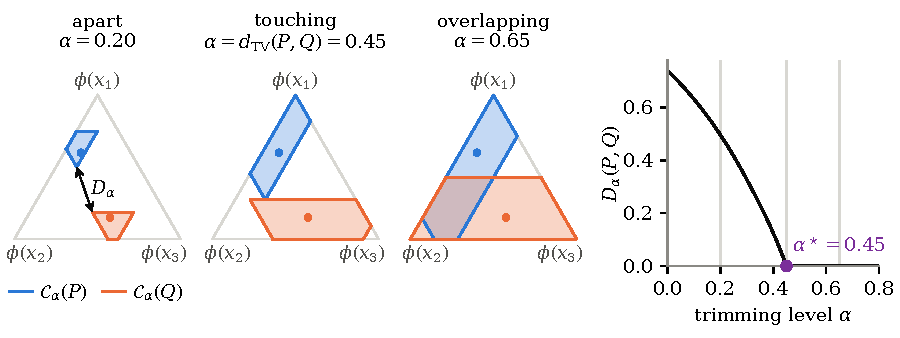
\includegraphics[width=\textwidth]{figs_print/fig0_regions.pdf}
\caption{Left: the regions $\mathcal C_\alpha(P)$ and $\mathcal C_\alpha(Q)$ of laws with weights $(\regWeightsP)$ and
$(\regWeightsQ)$ on three points whose feature vectors are unit vectors at $120$ degrees in the plane, drawn
isometrically (untrimmed embeddings as dots), at $\alpha=\regAlphaLo$, at $\alpha=\TV(P,Q)=\regTV$ and at
$\alpha=\regAlphaHi$. Right: the distance $D_\alpha(P,Q)$, computed exactly, with these levels marked.}
\label{fig:regions}
\end{figure}

A closed convex set $A\subset\Hh$ is determined by its support function $h_A(f)=\sup_{a\in A}\langle a,f\rangle_\Hh$,
how far it reaches in the direction $f$. For the trimmed regions this function is a familiar risk measure, the
conditional value-at-risk of finance \citep{rockafellaruryasev2000}.

\begin{lemma}[Support function]
\label{lem:cvar}
Under Assumption~\ref{ass:regularity}, for every $f\in\Hh$,
\begin{equation}
h_{\mathcal C_\alpha(P)}(f)
=\sup_{0\le g\le\beta,\ \E_Pg=1}\E_P[g(X)f(X)]
=\inf_{t\in\R}\Big\{t+\beta\,\E_P\big[(f(X)-t)_+\big]\Big\},
\label{eq:cvar}
\end{equation}
the supremum is attained, and the second equality holds for every bounded measurable $f$.
\end{lemma}

The first equality is the reproducing property, and the right-hand side is the representation by
\citet{rockafellaruryasev2000} of the mean of $f(X)$ over the upper $(1-\alpha)$-fraction of its distribution, an atom
at the cut being split. The lemma is the RKHS instance of the defining property of zonoid trimmed regions
\citep{koshevoy1997zonoid,dyckerhoff2011weighted}.

Maximizing $\E_P[gf]$ over trimming densities is a bathtub problem, whose solution $g$ fills its cap $\beta$ on the
largest values of $f$ until the mass runs out and is zero below. In a fixed direction the optimal trimming therefore
keeps the part of the law on one side of a cut, the level set $\{f\ge t\}$ with $t$ the $\alpha$-quantile of $f(X)$,
and the minimizing $t$ in \eqref{eq:cvar} is that cut.

For each fixed $t$, moreover, the expression inside the infimum is an ordinary mean, of the bounded function
$t+\beta(f-t)_+$. A region is thus a family of trimmed means, one per direction, and a trimmed mean is an infimum of
ordinary means. Means of bounded functions, and of bounded vectors of $\Hh$, concentrate at the rate $n^{-1/2}$ with
constants that depend only on the bound $\kappa$, and this rate cannot be improved for the mean embedding or the MMD
\citep{tolstikhin2016minimax,tolstikhin2017minimax}. Every finite-sample validity statement below reduces to such
means, and the empirical regions are uniformly close to the population ones,
\begin{equation}
\sup_{0\le\alpha<1}(1-\alpha)\,d_H\big(\mathcal C_\alpha(P_n),\mathcal C_\alpha(P)\big)
\le\kappa\Big[\frac4{\sqrt n}+\sqrt{\frac{2\log(2/\delta)}n}\,\Big]
\label{eq:hausdorff}
\end{equation}
with probability at least $1-\delta$, for every $P$, where $d_H$ is the Hausdorff distance in $\Hh$
(Corollary~\ref{cor:uniform} of the supplement). No complexity of the sample space enters \eqref{eq:hausdorff}, because the
regions live in $\Hh$ and the kernel bound $\kappa$ is their only constant.

\subsection{The statistic, its witness and the trimming it selects}
\label{sec:statistic}

The statistic is $\widehat D_\alpha\coloneqq D_\alpha(P_n,Q_m)$, and $\alpha\mapsto\widehat D_\alpha$ is the empirical
path. By Proposition~\ref{prop:georep} it is the distance between two polytopes, the square root of
\begin{equation}
\widehat D_\alpha^{\,2}
=\min_{w,v}\big\{w^\top K_{XX}w+v^\top K_{YY}v-2w^\top K_{XY}v\big\}
\label{eq:qp}
\end{equation}
over the capped simplices $0\le w_i\le\beta/n$, $\sum_iw_i=1$ and $0\le v_j\le\beta/m$, $\sum_jv_j=1$, where $K_{XX}$,
$K_{YY}$ and $K_{XY}$ are the Gram matrices. The objective is $\|\sum_iw_i\phi(X_i)-\sum_jv_j\phi(Y_j)\|_\Hh^2$, so
\eqref{eq:qp} is a convex quadratic program, the problem of the nearest points of two reduced convex hulls, which is the
dual of the $\nu$-support vector machine \citep{bennett2000duality,crisp1999geometric,takeda2008nusvm}. The witness
below is the normal of its hyperplane, and Proposition~\ref{prop:bangbang} is the structure of its support vectors read
as a trimming. We solve it by accelerated projected gradient (Section~\ref{sec:computationdetails} of the supplement). For a minimizer $(w,v)$, the \emph{witness}, the name that \citet{gretton2012kernel} use at $\alpha=0$, is
the difference of the two closest points,
\begin{equation}
\widehat d=\sum_iw_i\phi(X_i)-\sum_jv_j\phi(Y_j),
\qquad
\widehat d(x)=\sum_iw_ik(X_i,x)-\sum_jv_jk(Y_j,x).
\label{eq:witness}
\end{equation}
It is a function on $\mathcal X$, large where the trimmed first sample has more mass than the trimmed second, and it
can be evaluated at points not used to compute it. Its direction $\widehat f=\widehat d/\widehat D_\alpha$, with $\widehat f=0$ when $\widehat D_\alpha=0$,
separates the two empirical regions. The population witness $d^\star$ is the element of minimal norm of
$\mathcal C_\alpha(P)-\mathcal C_\alpha(Q)$, with direction $f^\star=d^\star/D_\alpha(P,Q)$.

Let $\mathcal T_\alpha$ be the set of minimizers $(w,v)$ of \eqref{eq:qp}. Each of them is a pair of trimmed samples,
since the weighted empirical measures $P_n^w=\sum_iw_i\delta_{X_i}$ and $Q_m^v=\sum_jv_j\delta_{Y_j}$ are
$\alpha$-trimmings of $P_n$ and $Q_m$ whose embeddings are at distance $\widehat D_\alpha$. The witness determines
them.

\begin{proposition}[Structure of the empirical trimming]
\label{prop:bangbang}
The set $\mathcal T_\alpha$ is nonempty, convex and compact. Moreover:
\begin{enumerate}[label=(\roman*),leftmargin=*]
\item the difference $\widehat d=\sum_iw_i\phi(X_i)-\sum_jv_j\phi(Y_j)$ takes the same value at every
$(w,v)\in\mathcal T_\alpha$, namely the element of minimal norm of $\mathcal C_\alpha(P_n)-\mathcal C_\alpha(Q_m)$, and
$\|\widehat d\|_\Hh=\widehat D_\alpha$;
\item if $\widehat D_\alpha>0$, let $n_{1-\alpha}=\lfloor n(1-\alpha)\rfloor$ and let $\widehat t_n$ be the
$(n_{1-\alpha}+1)$-th smallest of the values $\widehat d(X_1),\dots,\widehat d(X_n)$, with $\widehat t_n=+\infty$ if
$n_{1-\alpha}=n$. Then every $(w,v)\in\mathcal T_\alpha$ has $w_i=\beta/n$ when $\widehat d(X_i)<\widehat t_n$ and $w_i=0$
when $\widehat d(X_i)>\widehat t_n$, the observations with $\widehat d(X_i)=\widehat t_n$ sharing the remaining mass.
Symmetrically, with $m_{1-\alpha}=\lfloor m(1-\alpha)\rfloor$, $v_j=\beta/m$ when $\widehat d(Y_j)$ is above the
$(m_{1-\alpha}+1)$-th largest of the values $\widehat d(Y_1),\dots,\widehat d(Y_m)$, $v_j=0$ when it is below, and the ties
share the remainder;
\item if $\widehat D_\alpha=0$, then $\mathcal T_\alpha$ is the set of all feasible $(w,v)$ with
$\sum_iw_i\phi(X_i)=\sum_jv_j\phi(Y_j)$.
\end{enumerate}
\end{proposition}

Part (ii) is the bathtub of Lemma~\ref{lem:cvar} in the direction of the witness. Once $\widehat d$ is fixed the
problem is linear: the weights on the $X$'s minimize $\sum_iw_i\widehat d(X_i)$ over the capped simplex, and those on
the $Y$'s maximize $\sum_jv_j\widehat d(Y_j)$. So every optimal trimming of the first sample keeps at full weight the
observations on which the witness is smallest, the most $Q$-like ones, discards those above the cut and splits weight
only among ties at the cut, and the trimming of the second sample is the level set above a cut of the same function.
The cuts reappear in the betting test of Section~\ref{sec:split}. Part (iii) does not arise for $\alpha<1$ with a
strictly positive definite kernel and pairwise distinct pooled observations $X_1,\dots,X_n,Y_1,\dots,Y_m$, since the
feature vectors are then linearly independent and the minimizer is unique. Many observations may still share the cut,
as support vectors share the margin of a $\nu$-support vector machine, and with the Laplace kernel on the line all the
$X$'s whose witness values have rank $\lceil n(1-\alpha)\rceil$ or higher share it (Lemma~\ref{lem:lapclip} of the
supplement). For kernels whose empirical regions can meet we return the minimizer closest to uniform
weights (Section~\ref{sec:computationdetails} of the supplement).

\subsection{No informative upper bound}
\label{sec:upper}

By \eqref{eq:zeroeq}, $\TV(P,Q)>\alpha$ exactly when the regions are apart, and Sections~\ref{sec:analytic}
and~\ref{sec:split} certify this by lower confidence bounds valid on any sample space. We certify only from below
because no upper confidence bound on $\TV(P,Q)$ can be valid for all pairs of laws and still informative, as
\citet[Theorem~1.1]{horebarber2026blurred} prove for $\TV$ and \citet[Theorem~9]{blanchard2010semi} for mixture
proportions, in a line that goes back to \citet{bahadursavage1956} and \citet{donoho1988onesided}. The version below
holds even for laws on $[0,1]$ with densities bounded by $2$, and its conclusion is at $P=Q$.

\begin{theorem}[No informative upper bound, even for bounded densities]
\label{thm:impossible}
Fix $n,m\ge1$ and $\delta\in(0,1)$, and let $\mathcal P_2$ be the set of pairs of probability measures on $[0,1]$
whose densities with respect to Lebesgue measure are bounded by $2$. Suppose that
$\widehat U=\widehat U(X_{1:n},Y_{1:m})$, measurable and possibly randomized, satisfies
$\Pp_{P,Q}(\TV(P,Q)\le\widehat U)\ge1-\delta$ for every $(P,Q)\in\mathcal P_2$. Then, with $P_{\mathrm u}$ the uniform
law on $[0,1]$, $\Pp_{P_{\mathrm u},P_{\mathrm u}}(\widehat U\ge1)\ge1-\delta$.
\end{theorem}

A fixed kernel is blind in the same way: densities that oscillate ever faster stay at total variation $\tfrac12$ from
the uniform law while their MMD to it tends to zero (Section~\ref{sec:upperimposs} of the supplement). An upper end
needs an assumption, such as a margin with known constants, since $D_\alpha(P,Q)\ge c_0(\alpha^\star-\alpha)^\gamma$
gives $\alpha^\star\le\alpha+(\check D_\alpha/c_0)^{1/\gamma}$ for any $\check D_\alpha\ge D_\alpha(P,Q)$, or a blurred
version of $\TV$, and the data do not identify $c_0$ and $\gamma$. Lower bounds escape the argument, because rejecting
$\TV(P,Q)\le\alpha$ needs only one set on which the samples differ, but their rates do not: a valid lower bound with a
rate uniform over $\mathcal P_2$ would give an informative upper bound, so some restriction such as the margin is needed
for any rate.

\section{Testing a trimmed null, and an analytic baseline}
\label{sec:analytic}

For each level $\alpha\in[0,1)$ we test
\begin{equation}
H_{0,\alpha}:\ \TV(P,Q)\le\alpha
\qquad\text{against}\qquad
H_{1,\alpha}:\ \TV(P,Q)>\alpha ,
\label{eq:null}
\end{equation}
and by \eqref{eq:zeroeq} the null holds exactly when $D_\alpha(P,Q)=0$. The null is a total-variation neighborhood of
$P=Q$, a relevant hypothesis in the sense of \citet{dettekokotaue2020}, as in the trimming-based tests of
\citet{alvarez2012similarity} and \citet{delbarrio2020ks} and in robust tests between neighborhoods of laws
\citep{huber1965robust,huber1973minimax,schrab2025robust,liubriol2025robust}, which fix its size in advance, whereas
here it is the quantity to be estimated. Kernel tests of composite nulls \citep{key2025composite} calibrate over a
parametric family, and equivalence tests \citep{wellek2010equivalence} put such a neighborhood in the alternative
(Section~\ref{app:analytic} of the supplement). This section gives a threshold $\tau(\alpha)$, computed before the
data, that $\widehat D_\alpha$ exceeds with probability at most $\delta$ under every pair in the null. Inverted over
$\alpha$, it gives a baseline that needs no split but far more observations than our method.

\subsection{A threshold for the whole null}

Limit laws are of little help in calibrating $\widehat D_\alpha$, because at the boundary of the null the two regions
touch, and a minimum over trimmings is then only directionally differentiable in the laws, with a limit law that
depends on the unknown geometry of the contact \citep{fang2019inference}, and permutation is exact only under $P=Q$. We
bound $\widehat D_\alpha$ instead by a difference of sample means. Under $H_{0,\alpha}$ the laws share an
$\alpha$-trimming $R$ by \eqref{eq:tvintersect}, with densities $g_P=dR/dP$ and $g_Q=dR/dQ$ bounded by $\beta$, so the
weights $w_i=g_P(X_i)/n$ and $v_j=g_Q(Y_j)/m$ respect the caps of \eqref{eq:qp}, and the embeddings they give are
averages of independent vectors with the same mean $\mu_R$. Their totals fluctuate around one, and rescaling the weights,
or adding mass under the caps, gives a feasible pair at the price of a term proportional to the shortfalls
(Lemma~\ref{lem:plugin} of the supplement). So $\widehat D_\alpha$ is at most the norm of a centered difference of two
averages of vectors bounded by $\beta\kappa$, plus two shortfalls, and bounded-difference and Bernstein inequalities
give a threshold in closed form. Let $n_\star=nm/(n+m)$, so that $1/n_\star=1/n+1/m$, $c=\max(1/n,1/m)$, $L=\log(6/\delta)$ and $\bar\kappa^2=\min(\kappa^2,\Delta_\phi^2/2)$.

\begin{theorem}[Plug-in threshold]
\label{thm:plugin}
Let (A1) and (A2) of Assumption~\ref{ass:regularity} hold, and let
\begin{gather*}
\tau^{\mathrm P}(0)=\bar\kappa/\sqrt{n_\star}+\Delta_\phi\sqrt{\log(1/\delta)/(2n_\star)},\\
\tau^{\mathrm P}(\alpha)=\sqrt{\beta \bar\kappa^2/n_\star}+\beta \Delta_\phi\sqrt{L/(2n_\star)}+\Delta_\phi\Big[\sqrt{2(\beta-1)L/n_\star}+\frac{cL}3\Big]
\qquad(0<\alpha<1).
\end{gather*}
Then for every $\alpha\in[0,1)$, $n,m\ge1$, $\delta\in(0,1)$ and every pair with $\TV(P,Q)\le\alpha$,
$\Pp\big(\widehat D_\alpha>\tau^{\mathrm P}(\alpha)\big)\le\delta$. Moreover, $\alpha\mapsto\tau^{\mathrm P}(\alpha)$
is nondecreasing on $[0,1)$.
\end{theorem}

The threshold depends on $\kappa$, $\Delta_\phi$, $\alpha$, $n$, $m$ and $\delta$ alone and is, up to a term of order
$\Delta_\phi\log(1/\delta)/(n\wedge m)$, of order $\beta \Delta_\phi\{(1+\log(1/\delta))/(n\wedge m)\}^{1/2}$. It
jumps up at $0+$, where $L>\log(1/\delta)$ replaces $\log(1/\delta)$. The pair enters only through the existence of $R$. At
$\alpha=0$ the common trimming is $R=P=Q$, and Theorem~\ref{thm:plugin} is a finite-sample bound on the MMD of the
kind given by \citet[Corollary~9]{gretton2012kernel}. For the Gaussian kernel and $n=m$ it reads
$\tau^{\mathrm P}(0)=[1+\sqrt{\log(1/\delta)}\,]\sqrt{2/n}$.

We write $\tau=\tau^{\mathrm P}$ for the threshold of the test. A second valid threshold $\tau^{\mathrm S}(\alpha,\delta)$
comes from the two-sided bound of Theorem~\ref{thm:twosided} of the supplement, by the same reduction to means as
\eqref{eq:hausdorff}, but it is larger than $\tau^{\mathrm P}$ at the sample sizes we use. Since $\tau$ is
nondecreasing and the empirical path is nonincreasing, one event serves every level.

\begin{lemma}[One event for all levels]
\label{lem:oneevent}
Let $\tau:[0,1)\to[0,\infty)$ be nondecreasing, and suppose that $\Pp(\widehat D_\alpha>\tau(\alpha))\le\delta$ for
every $\alpha$ and every pair with $\TV(P,Q)\le\alpha$. Then for every pair with $\alpha^\star<1$, the event
$\{\widehat D_{\alpha^\star}\le\tau(\alpha^\star)\}$ has probability at least $1-\delta$, and on it
$\widehat D_\alpha\le\tau(\alpha)$ for every $\alpha\in[\alpha^\star,1)$.
\end{lemma}

The analytic test rejects $H_{0,\alpha}$ when
\begin{equation}
\widehat D_\alpha>\tau(\alpha) .
\label{eq:test}
\end{equation}
It has level $\delta$ for all $n,m\ge1$, uniformly over the null, by Lemma~\ref{lem:oneevent} one event carries the
guarantee for all levels at once, and its level does not use (A3). Its validity at every sample size, uniformly over the null, answers
the question of \citet{alvarez2012similarity} recalled in the introduction, as does, more simply, the betting test of
Section~\ref{sec:split}. The kernel must be fixed before the data are seen, for instance on a held-out pilot sample
(Section~\ref{sec:data}). One threshold for every pair in the null is a worst case: at the boundary of a
two-dimensional design, at $n=m=300$ and $\alpha=\alpha^\star$, $\tau(\alpha)$ is $\stCalibRatioTauP$ times the
empirical $1-\delta$ quantile of $\widehat D_\alpha$ (Section~\ref{app:experiments} of the supplement).

\subsection{The estimator}
\label{sec:alpha}

Inverting the test over $\alpha$, we define the analytic estimator, with a subscript that sets it apart from the
split-sample bound $\widehat\alpha$ of Section~\ref{sec:lower},
\begin{equation}
\widehat\alpha_{\mathrm{an}}\coloneqq\inf\big\{\alpha\in[0,1):\ \widehat D_\alpha\le\tau(\alpha)\big\} ,
\label{eq:alphaest}
\end{equation}
the first level at which the empirical path falls below the threshold. Since $\alpha\mapsto\widehat D_\alpha$ is
nonincreasing and $\tau$ nondecreasing, every level above $\widehat\alpha_{\mathrm{an}}$ is accepted and every level below it rejected,
so bisection brackets $\widehat\alpha_{\mathrm{an}}$. It is well defined, because
$\widehat D_\alpha\le \Delta_\phi$ while $\tau(\alpha)\to\infty$ as $\alpha\to1$ when $\Delta_\phi>0$. On the event of
Lemma~\ref{lem:oneevent}, of probability at least $1-\delta$ whenever $\alpha^\star<1$, every level from $\alpha^\star$
on is accepted, so $\widehat\alpha_{\mathrm{an}}\le\alpha^\star$ and every rejected level lies below $\alpha^\star$, at every sample
size, for every pair and however the levels tested were chosen. A grid of levels read upward, as in
Section~\ref{sec:data}, therefore gives a lower confidence bound too. It is consistent from below,
$\Pp(\widehat\alpha_{\mathrm{an}}<\alpha)\to0$ for $\alpha<\alpha^\star$, as $\widehat D_\alpha\ge
D_\alpha-\tau^{\mathrm S}(\alpha,\delta')$ with probability $1-\delta'$ (Theorem~\ref{thm:twosided} of the supplement)
and both thresholds tend to zero.

\subsection{How many observations}
\label{sec:samplesize}

Because $\tau$ does not depend on the data, the sample size at which the test fires can be computed before any data
are collected, given a guess at the effect. For the Gaussian kernel and $n=m$, Theorem~\ref{thm:plugin} gives
$\tau(0)\le C_0\sqrt{2/n}$, so the test rejects $H_{0,0}$ as soon as
\begin{equation}
n>2\Big(\frac{C_0}{\widehat D_0}\Big)^2,
\qquad
C_0=\bar\kappa+\Delta_\phi\sqrt{\log(1/\delta)/2}=1+\sqrt{\log(1/\delta)}\approx\cstCzero
\ \text{ at }\delta=0.05 .
\label{eq:samplesize}
\end{equation}
With a guess at $D_0=\MMD(P,Q)$ in place of $\widehat D_0$, \eqref{eq:samplesize} is a design rule, which scales like
$D_0^{-2}$.

\section{The split-sample lower bound}
\label{sec:split}

The threshold of Section~\ref{sec:analytic} is a worst case over the whole null. Our method avoids it: we fit the
witness and its two cuts on part of the data and test a fixed function on the rest, refitting on each batch. The
batches and the number of bets are fixed in advance, so the test is valid at every sample size but not anytime-valid.
Validity rests on one inequality, $\E_P\rp-\E_Q\rp\le\TV(P,Q)$ for every $\rp$ with values in $[0,1]$, as in the
framework of \citet{naf2022hplb}, with the clipped witness in the role of their classifier.

\subsection{A ramp of the witness}
\label{sec:ramp}

Any unit vector $f\in\Hh$ gives a lower bound on the distance between two sets $A,B\subset\Hh$,
\[
\dist(A,B)\ge\mathrm{sep}(f;A,B)\coloneqq\inf_{a\in A}\langle f,a\rangle_\Hh-\sup_{b\in B}\langle f,b\rangle_\Hh ,
\]
with equality when $A,B$ are convex and weakly compact, $\dist(A,B)>0$, and $f$ is the direction of the minimal-norm
difference (Lemma~\ref{lem:separation} of the supplement). A direction chosen from data is therefore harmless once it
is independent of the data on which it is evaluated. For the trimmed regions both terms of $\mathrm{sep}$ are trimmed
means by Lemma~\ref{lem:cvar}, of $f(X)$ over the lower and of $f(Y)$ over the upper $(1-\alpha)$-fraction of its
distribution. A trimmed mean is cut at a quantile, which depends on the data and makes it hard to calibrate. With the cut fixed in advance it becomes an ordinary mean, as in the second reading of Lemma~\ref{lem:cvar}. For a bounded
measurable $f$ and reals $t,u$ put
\[
\theta(f;t,u)\coloneqq\E_P\big[t-\beta(t-f(X))_+\big]-\E_Q\big[u+\beta(f(Y)-u)_+\big].
\]

\begin{lemma}[Cut points turn the separation into a ramp]
\label{lem:ramp}
Let $f$ be bounded and measurable and $\alpha\in[0,1)$. Then:
\begin{enumerate}[label=(\roman*),leftmargin=*]
\item $\theta(f;t,u)\le\inf_{P'\in R_\alpha(P)}\E_{P'}f-\sup_{Q'\in R_\alpha(Q)}\E_{Q'}f$ for all reals $t,u$; the
supremum of the left side over $(t,u)$ equals the right side and is attained at a $(1-\alpha)$-quantile of $f(X)$
and an $\alpha$-quantile of $f(Y)$; and for $f$ in the unit ball of $\Hh$ the right side is
$\mathrm{sep}(f;\mathcal C_\alpha(P),\mathcal C_\alpha(Q))$;
\item if $t>u$, then with the clipped witness $\tilde f=(f\vee u)\wedge t$ and the ramp $\rp=(\tilde f-u)/(t-u)$, which
takes values in $[0,1]$, $\theta(\tilde f;t,u)=\beta(t-u)\big(\E_P\rp-\E_Q\rp-\alpha\big)\ge\theta(f;t,u)$;
\item every measurable $\rp$ with values in $[0,1]$, the ramp in particular, has $\E_P\rp-\E_Q\rp\le\TV(P,Q)$.
\end{enumerate}
\end{lemma}

In practice $f$ is the witness direction $\widehat f$. The \emph{clipped witness} $\tilde f$ is $f$ with its values
below $u$ raised to $u$ and above $t$ lowered to $t$, and the \emph{ramp} $\psi$ rescales it to $[0,1]$, a soft
classifier, as the witness is large where $P$ has more mass. By part (i), the trimmed separation in direction $f$ is the
largest value of $\theta(f;t,u)$ over the cut points, attained at the cuts of Proposition~\ref{prop:bangbang}, and once
these are fixed $\theta$ is a difference of two ordinary means. By part (ii), clipping never lowers $\theta$ and turns
it into a positive multiple of $\E_P\psi-\E_Q\psi-\alpha$, which by part (iii) never exceeds $\TV(P,Q)-\alpha$. So,
with the cut points fixed, a test that rejects $\E_P\psi-\E_Q\psi\le\alpha$ shows that $\TV(P,Q)>\alpha$, with no
further assumption on the laws.

\subsection{A betting test}
\label{sec:betting}

The test of $\E_P\psi-\E_Q\psi\le\alpha$ must use data that played no part in choosing $\psi$, and it should keep its
level at every sample size. We obtain both by splitting the samples. Before the data are examined, each sample is put in
a random order and cut into three batches, the first quarter (batch $0$), the second quarter (batch $1$) and the second
half (batch $2$). Batch $0$ is used only for fitting, and
batches $1$ and $2$ are bet on, each with a function fitted on the batches before it. Any number of batches at fractions
fixed in advance would do (Section~\ref{sec:bettingdetails} of the supplement).

Before betting on batch $b\in\{1,2\}$, we solve \eqref{eq:qp} at level $\alpha$ on the batches before it and take the
witness direction $\widehat f_b$. Its cut points are those at which a trimming at level $\alpha$ would cut: the
smallest $(1-\alpha)$-quantile $\widehat t_b$ of its values at the $X$'s of those batches, their
$\lceil n_{<b}(1-\alpha)\rceil$-th order statistic, and the largest $\alpha$-quantile $\widehat u_b$ of its values at
their $Y$'s, the $(\lfloor m_{<b}\alpha\rfloor+1)$-th, where $n_{<b},m_{<b}$ are the sizes of the batches before $b$.
Each value is computed without the point's own term in \eqref{eq:witness}, which pulls the value at a fitting point
toward its own sample, and removing it is a cheap leave-one-out correction of the in-sample bias of these quantiles.
If $\widehat t_b>\widehat u_b$, let $\psi_b$ be the ramp of $\widehat f_b$ between $\widehat u_b$ and $\widehat t_b$;
otherwise batch $b$ is skipped.

Within batch $b$ each $X$ is paired with a block of $Y$'s (or the reverse when the $Y$'s are fewer), and each pair
gives $Z=\psi_b(X)-\overline{\psi_b(Y)}$, the bar being the mean over the block. Given the earlier batches, $Z$ takes
values in $[-1,1]$ and has mean $\E_P\psi_b-\E_Q\psi_b$, at most $\alpha$ under $H_{0,\alpha}$ by
Lemma~\ref{lem:ramp}(iii). The pairs of both batches, numbered $k=1,\dots,N$, number about $\tfrac34\min(n,m)$, fixed
before any data are seen. A gambler starts with wealth $K_0=1$ and at pair $k$ stakes a fraction $\lambda_k$ of
the current wealth on $Z_k$ exceeding $\alpha$,
\[
K_k=K_{k-1}\{1+\lambda_k(Z_k-\alpha)\}=\prod_{l\le k}\{1+\lambda_l(Z_l-\alpha)\}.
\]
When the fitted ramp has $\E_P\rp_b-\E_Q\rp_b>\alpha$, as it does below $\alpha^\star$ for large samples
(Proposition~\ref{prop:loconsistency}), the logarithm of the wealth grows linearly in $k$ with well-chosen fractions.
The test rejects
$H_{0,\alpha}$ as soon as the wealth reaches $1/\delta$. Each fraction $\lambda_k\in[0,\lambda_{\max}/(1+\alpha)]$,
$\lambda_{\max}\in(0,1]$, may depend on earlier batches and pairs only, and the bound keeps the wealth nonnegative.
Such fitting rules and fractions are called predictable (Section~\ref{sec:bettingdetails} of the supplement). Ours stake more when the earlier pairs vary little, through a
running estimate of their variance started from the variance of the ramp on the fitting batches
(Equation~\eqref{eq:fractions} of the supplement). Algorithm~\ref{alg:split} lists the method with
every default.

\begin{theorem}[Validity of the betting test]
\label{thm:betting}
Let $X_1,\dots,X_n$ be i.i.d.\ $P$ and $Y_1,\dots,Y_m$ i.i.d.\ $Q$, the two samples independent, cut into batches as
above. Fix $\alpha\in[0,1)$ and $\delta\in(0,1)$. For every predictable fitting rule and fractions, all sample sizes and
every pair with $\TV(P,Q)\le\alpha$,
\[
\Pp\Big(\max_{k\le N}K_k\ge1/\delta\ \Big|\ \text{batch }0\Big)\le\delta .
\]
Hence rejecting $H_{0,\alpha}$ when $\max_{k\le N}K_k\ge1/\delta$ has level at most $\delta$ for every sample size,
uniformly over $H_{0,\alpha}$, with no assumption on the laws, the kernel or the witness, and a rejection shows that
$\TV(P,Q)>\alpha$.
\end{theorem}

Given the earlier batches and pairs, $\E Z_k\le\alpha$ by Lemma~\ref{lem:ramp}(iii), so $K_k$ is a nonnegative
supermartingale started at one, and the maximal inequality of \citet{ville1939} bounds the probability that it ever
reaches $1/\delta$. The test is the two-sample test by betting of \citet{shekhar2024nonparametric}, with the ramp as
the predictable function and the null $\E_P\rp-\E_Q\rp\le\alpha$ in place of $P=Q$. Any function with
values in $[0,1]$ fitted on earlier batches may replace the ramp, such as the predicted labels or probabilities of a
classifier; \citet{podkopaev2023sequential} bet on classifiers in this way in their predictive tests, and
Section~\ref{sec:numharder} compares such classifiers with the ramp. Betting tests of a tolerance on a difference of means audit fairness
\citep{chugg2023auditing}, and \citet{pandeva2024deep} bet with learned functions on nulls defined by operators. Unlike
these and \citet{shekhar2024nonparametric}, our test fixes $N$ and the batches in advance, and $\lambda_k$ depends on
$N$. Our fractions, adapted from \citet[Remark~1]{waudbysmith2024estimating} with $\lambda_{\max}=\tfrac12$, are
explicit and enter the rates of Section~\ref{sec:rates}. Against a small effect, at $\delta=0.05$ and power $0.8$, the
betting test needs, heuristically, about $\cstBetRatioEighty$ times as many bet-on pairs as a test calibrated by the
central limit theorem, and the quarter of each sample used only for fitting comes on top
(Section~\ref{sec:bettingdetails} of the supplement). Online Newton steps or mixtures over fractions may recover part
of this loss.

\subsection{The lower confidence bound}
\label{sec:lower}

Running the test of Theorem~\ref{thm:betting} on a grid of levels gives our lower confidence bound on $\alpha^\star$, the
split-sample bound $\widehat\alpha$.

\begin{corollary}[Lower confidence bound for the contamination level]
\label{cor:lower}
Fix a grid $\alpha_1<\dots<\alpha_J$ in advance, test each $H_{0,\alpha_j}$ by Theorem~\ref{thm:betting} on the same
batches, with any fitting rule at each level, and read the grid upward, stopping at the first failure:
\begin{equation}
\widehat\alpha\coloneqq\max\big\{\alpha_j:\ H_{0,\alpha_i}\text{ is rejected for every }i\le j\big\},
\label{eq:downclosed}
\end{equation}
with $\widehat\alpha=0$ if $H_{0,\alpha_1}$ is not rejected. Then
$\Pp(\widehat\alpha>\TV(P,Q))\le\delta$ for all sample sizes and every pair $(P,Q)$, with no
multiplicity correction. Moreover, the probability that $H_{0,\widehat\alpha}$ is rejected and
$\TV(P,Q)\le\widehat\alpha$ is at most $\delta$, so a rejected $\widehat\alpha$ shows
$\TV(P,Q)>\widehat\alpha$.
\end{corollary}

When the grid starts at $\alpha_1=0$, the value $\widehat\alpha=0$ means either that $H_{0,0}$ was rejected, which
shows $\TV(P,Q)>0$, or that nothing was rejected, and we report which. Only the first true null on the grid can make
$\widehat\alpha$ too large, which is why no correction is needed, whereas bisection could test several true nulls, as
the refitted ramp may accept a level and reject a larger one. The grid may be chosen from batch $0$
(Remark~\ref{rem:batch0grid} of the supplement). The bound is of the kind of the lower bound of
\citet[Theorem~7]{blanchard2010semi} on a mixture proportion, with one function fitted on earlier batches in place of
their uniform bound over a class, so no complexity term enters. With a witness fitted at each level it is also
consistent, up to the grid.

\begin{proposition}[Consistency of the lower bound]
\label{prop:loconsistency}
Let Assumption~\ref{ass:regularity} hold, and compute $\widehat\alpha$ with a kernel fixed before the data are seen,
an exact minimizer of \eqref{eq:qp} at each level, cut points within one rank of the quantiles of
Section~\ref{sec:betting} (Equation~\eqref{eq:cutrank} of the supplement), and the fractions of
Section~\ref{sec:betting} with their running variance estimate floored at a constant $v^2_{\min}\in(0,4]$ that does
not depend on $n,m$. Let $\alpha_{j^\star}=\max\{\alpha_j:\alpha_j<\alpha^\star\}$,
or $0$ if no level is below $\alpha^\star$. Then $\Pp(\widehat\alpha>\alpha_{j^\star})\le\delta$ for all
$n,m$, and $\Pp(\widehat\alpha<\alpha_{j^\star})\to0$ as $n,m\to\infty$; if $\alpha^\star$ is not a grid
level, also $\Pp(\widehat\alpha>\alpha_{j^\star})\to0$. On grids fixed in advance whose mesh tends to
zero, with $\log J=o(n\wedge m)$, $\widehat\alpha\to\alpha^\star$ in probability.
\end{proposition}

Below $\alpha^\star$ the excess of the population ramp over $\alpha$ is at least $D_\alpha/(\beta \Delta_\phi)$
(Lemma~\ref{lem:popramp} of the supplement), once the fitting batches are large the fitted ramp keeps half of this
excess, with no density condition, and betting has power tending to one against a fixed excess. Fitting the witness at
the level tested matters here. A single witness fitted at $\alpha=0$, the one a test of $P=Q$ would use, is valid and cheaper but need not be consistent:
Section~\ref{sec:alphazero} of the supplement gives laws with $\TV(P,Q)=\loExTV$ on which every ramp of its limit has
$\E_P\rp-\E_Q\rp\le\loExKS$.

The proposition, like the rates of Section~\ref{sec:rates}, assumes a kernel fixed in advance and exact minimizers,
and its constants grow like $1/v^2_{\min}$ through the bound $\lambda_k\le\{2\log(1/\delta)/(Nv^2_{\min})\}^{1/2}$, an
artifact of the proof, as the fractions keep the quadratic term of the wealth of order $\log(1/\delta)$ once the
running variance tracks the second moment. Our runs use the floor $10^{-8}$, a median-distance
bandwidth computed on the fitting batches, and accelerated projected gradient stopped at a relative tolerance
(Algorithm~\ref{alg:split} of the supplement). Validity is unaffected, but for these runs Proposition~\ref{prop:loconsistency} and
Theorems~\ref{thm:loratemain} and~\ref{thm:laplacerate} describe the trend only.

\section{Rates and optimality}
\label{sec:rates}

The error $\alpha^\star-\widehat\alpha$ is parametric on a grid of matching mesh when a function of the RKHS
separates the two contaminations, and no valid lower bound does better over such pairs (Section~\ref{sec:bothrates}). When they touch, a margin argument guarantees slower rates that depend on
the kernel, polynomial for Sobolev kernels and logarithmic for the Gaussian kernel (Sections~\ref{sec:linearmargin}
and~\ref{sec:touching}). The excess of the bound's own ramp recovers the parametric rate up to logarithmic factors on
the line with the Laplace kernel, for densities that cross once and under a condition on their likelihood ratio
(Theorem~\ref{thm:laplacerate}).

\subsection{A margin condition}
\label{sec:rate}

A rate needs a condition on the pair, and we use one, on how fast the regions separate below $\alpha^\star$.

\begin{assumption}[Polynomial margin]
\label{ass:margin}
There are constants $c_0>0$ and $\gamma\ge1$ such that $D_{\alpha^\star-\epsilon}(P,Q)\ge c_0\,\epsilon^\gamma$ for
all $\epsilon\in[0,\alpha^\star]$.
\end{assumption}

Validity and consistency hold for every pair, but by Section~\ref{sec:upper} no rate holds uniformly over all pairs,
and Assumption~\ref{ass:margin} restricts the pair only through its path. It suffices for $\epsilon\le\epsilon_0$, as the path is
nonincreasing, with $c_0(\epsilon_0/\alpha^\star)^\gamma$ in place of $c_0$. A margin of some form always exists when
$0<\alpha^\star<1$ (Lemma~\ref{lem:marginexists} of the supplement), Proposition~\ref{prop:newrates} of the supplement
gives the rate under any margin, and the assumption adds the polynomial speed. Exponents below $1$ are excluded, because
the rescaled path $(1-\alpha)D_\alpha(P,Q)$ is convex (Lemma~\ref{lem:pathconvex} of the supplement), so the path
leaves zero at most linearly, with a kink ($\gamma=1$) or tangentially ($\gamma>1$). The linear case holds when a function of the RKHS
separates the two contaminations (Section~\ref{sec:linearmargin}) and, for laws with continuous densities and a
continuous kernel, only if they are apart. In the following example the separating function takes three values.

\begin{example}[Separated contamination]
\label{ex:separated}
Let (A1) and (A2) of Assumption~\ref{ass:regularity} hold. Let $R$, $P_0$ and $Q_0$ be probability measures
concentrated on pairwise disjoint measurable sets $S_R$, $S_P$ and $S_Q$, let $\alpha^\star\in(0,1)$, and put
$P=(1-\alpha^\star)R+\alpha^\star P_0$ and $Q=(1-\alpha^\star)R+\alpha^\star Q_0$. Then $\TV(P,Q)=\alpha^\star$. If
moreover some $f\in\Hh$ takes the value $0$ on $S_R$, $1$ on $S_P$ and $-1$ on $S_Q$, then for every
$\alpha\in[0,\alpha^\star]$,
\[
D_\alpha(P,Q)\ \ge\ \frac{2(\alpha^\star-\alpha)}{(1-\alpha)\|f\|_\Hh}\ \ge\ \frac{2(\alpha^\star-\alpha)}{\|f\|_\Hh},
\]
so Assumption~\ref{ass:margin} holds with $\gamma=1$ and $c_0=2/\|f\|_\Hh$.
\end{example}

Such an $f$ exists for finite sets and a strictly positive definite kernel, as in
Section~\ref{sec:regions}, and for Mat\'ern kernels when the sets are bounded and apart (Section~\ref{sec:exproof} of
the supplement).

\subsection{Linear and slower margins}
\label{sec:linearmargin}

Whether the margin is linear depends on whether the contaminations touch. Write $P=P\wedge Q+\alpha^\star P_0$ and $Q=P\wedge Q+\alpha^\star Q_0$, where the contaminations $P_0$ and $Q_0$ are
the probability measures with densities $(p-q)_+/\alpha^\star$ and $(q-p)_+/\alpha^\star$.

\begin{proposition}[Touching contaminations]
\label{prop:newslope}
Let (A1) and (A2) of Assumption~\ref{ass:regularity} hold and let $0<\alpha^\star<1$, let $\mathcal X$ be a topological
space with its Borel sets, and let $\phi$ be continuous, as it is for a continuous kernel. Then
\[
\lim_{\epsilon\downarrow0}\frac{(1-\alpha^\star+\epsilon)\,D_{\alpha^\star-\epsilon}(P,Q)}{\epsilon}
\ \le\ \inf\big\{\|\phi(x)-\phi(y)\|_\Hh:\ x\in\supp P_0,\ y\in\supp Q_0\big\} .
\]
If the supports of $P_0$ and $Q_0$ meet, the limit is $0$ and Assumption~\ref{ass:margin} fails with $\gamma=1$. They
meet when $\mathcal X$ is a connected open subset of $\R^d$ and $P\neq Q$ have continuous Lebesgue densities $p,q$
such that $\{p=q\}$ has empty interior, as for any two distinct finite mixtures of nondegenerate Gaussian laws.
\end{proposition}

The limit exists by Lemma~\ref{lem:pathconvex}(ii) of the supplement. At the level $\alpha^\star-\epsilon$ one may keep
$P\wedge Q$ and add mass $\epsilon$ of $P_0$ near a point $x$ to the first law and of $Q_0$ near $y$ to the second,
whose embeddings then differ by about $\epsilon\{\phi(x)-\phi(y)\}$. With continuous densities and kernel, a linear
margin thus needs an open set on which $p=q$ that separates $\{p>q\}$ from $\{q>p\}$, and for a Mat\'ern kernel and
$P_0$ with compact support disjoint supports of $P_0$ and $Q_0$ also suffice (Proposition~\ref{prop:newgammaone} of the
supplement). Overlapping smooth laws, such as the overlap and shift designs of Section~\ref{sec:numerical}, fall
outside the linear case.

When the contaminations touch, the path leaves zero tangentially, at a speed set by how well the RKHS approximates
the indicator of $A=\{p>q\}$, with $p,q$ densities with respect to $P+Q$. For measurable $f$ with $0\le f\le1$ let
$\mathrm{err}(f)=\int|\mathbf 1_A-f|\,d|P-Q|$, where $|P-Q|$ is the total variation measure of $P-Q$, so that
$\mathrm{err}(f)=\alpha^\star-(\E_Pf-\E_Qf)$, and $\mathrm{err}(f)/2$ is the excess risk of the randomized classifier
that assigns $x$ to $P$ with probability $f(x)$, in the balanced problem whose Bayes classifier is $\mathbf 1_A$.

\begin{proposition}[Margin from an approximate witness]
\label{prop:newapprox}
Let (A1) and (A2) hold and let $0<\alpha^\star<1$. For every $f\in\Hh$ with $0\le f\le1$ and $f\neq0$, and every
$\epsilon\in[0,\alpha^\star]$,
\[
D_{\alpha^\star-\epsilon}(P,Q)\ \ge\ \frac{\epsilon-\mathrm{err}(f)}{(1-\alpha^\star+\epsilon)\,\|f\|_\Hh} .
\]
Hence $D_{\alpha^\star-\epsilon}(P,Q)\ge\epsilon/\{2\mathcal W(\epsilon/2)\}$, where
$\mathcal W(t)=\inf\{\|f\|_\Hh:\ f\in\Hh,\ 0\le f\le1,\ \mathrm{err}(f)\le t\}$.
\end{proposition}

In particular, if some $f\in\Hh$ with $0\le f\le1$ equals $1$ $P_0$-almost surely and $0$ $Q_0$-almost surely,
then $\mathrm{err}(f)=0$, and Assumption~\ref{ass:margin} holds with $\gamma=1$ and $c_0=1/\|f\|_\Hh$, since
$1-\alpha^\star+\epsilon\le1$. This is what we mean by a function of the RKHS separating the two contaminations;
Example~\ref{ex:separated} gives the constant $2/\|f\|_\Hh$ for an $f\in\Hh$ equal to $0$ on the common component, $1$
on one contamination and $-1$ on the other.

A trimming at level $\alpha$, before it is renormalized, is a part $P'\le P$ of mass $1-\alpha$, so it lowers the
integral of a $[0,1]$-valued function under $P$ by at most $\alpha$ and does not raise it under $Q$, and the
reproducing property turns the remaining gap into a lower bound on $(1-\alpha)D_\alpha$. The function $\mathcal W$ is
the approximation error behind the rates of kernel classifiers \citep{smale2003estimating,steinwart2008svm}: the closer
$\alpha$ is to $\alpha^\star$, the sharper $f$ must be across $\{p=q\}$, and the smoother the kernel, the more this
costs in $\Hh$. For a single transversal crossing on the line, Sobolev and Gaussian kernels make this quantitative.

\begin{proposition}[Sobolev kernels]
\label{prop:newsobolev}
Let $\mathcal X=\R$ and $k(x,y)=k_0(x-y)$, with $k_0$ continuous and integrable and
$c(1+\xi^2)^{-s}\le\widehat{k_0}(\xi)\le C(1+\xi^2)^{-s}$ for some $s>1/2$, as for the Laplace kernel, with
$s=1$, and the Mat\'ern kernel of smoothness $s-1/2$. Let $P,Q$ have densities $p,q$ that are continuous near a
point $x_0$, with $p\ge q$ almost everywhere on $(x_0,\infty)$ and $p\le q$ almost everywhere on $(-\infty,x_0)$, $p-q$
differentiable at $x_0$ with
$(p-q)'(x_0)>0$, $p(x_0)>0$, and $|P-Q|(\{x:|x-x_0|>t\})\le C'e^{-t/C'}$ for some $C'$ and all $t>0$. Then there are
$0<c_1\le c_2$ such that for all small $\epsilon>0$,
\[
c_1\,\epsilon^{(2s+3)/4}\ \le\ D_{\alpha^\star-\epsilon}(P,Q)\ \le\ c_2\,\epsilon^{(2s+3)/4} .
\]
\end{proposition}

Assumption~\ref{ass:margin} therefore holds with $\gamma=(2s+3)/4$ and with no smaller exponent, $\gamma=5/4$ for the
Laplace kernel. For the lower bound, an indicator smoothed at width $w$ has $\mathrm{err}(f)$ of order $w^2$, as
$|p-q|$ vanishes linearly at $x_0$, and $\|f\|_\Hh$ of order $w^{1/2-s}$, and $w\asymp\epsilon^{1/2}$ balances the two, while
the upper bound comes from explicit trimmings whose difference has vanishing moments near $x_0$. For $s>d/2$ the lower
bound extends to $\R^d$ when $|P-Q|$ has compact support and $\{p>q\}$ has a smooth compact boundary, with the exponent $1+(2s-1)/\{2(r+1)\}$ when
$p-q$ vanishes at least to order $r$ there (Theorem~\ref{thm:newsobolev} and Corollary~\ref{cor:newsobolev} of the
supplement), which is sharp on the line, at least for $s<3/2$, when it vanishes exactly to order $r$
(Proposition~\ref{prop:newupperone} of the supplement).

\begin{proposition}[Gaussian kernel]
\label{prop:newgauss}
Let $P,Q$ satisfy the hypotheses of Proposition~\ref{prop:newsobolev} on the laws, put $\ell_0=(p-q)'(x_0)$, the slope of $p-q$ at $x_0$, and let
$k(x,y)=\exp\{-(x-y)^2/(2\sigma^2)\}$ on $\R$. For every $c>\pi^2\sigma^2\ell_0/8$ and every $j\ge1$ there are
$\epsilon_0>0$ and $C_j<\infty$ such that, for $0<\epsilon\le\epsilon_0$,
\[
\exp(-c/\epsilon)\ \le\ D_{\alpha^\star-\epsilon}(P,Q)\ \le\ C_j\,\epsilon^j .
\]
\end{proposition}

With the Gaussian kernel the path is thus flatter at $\alpha^\star$ than every power, yet a margin of exponential type holds.
The approximant is an indicator smoothed by a band-limited density, which lies in the Gaussian RKHS
\citep{steinwart2006explicit} with a norm that grows like $\exp(c/\epsilon)$.

\subsection{The rate, and when it is optimal}
\label{sec:bothrates}
\label{sec:optimality}

Under the margin the error of the bound is at most of order $(n\wedge m)^{-1/(2\gamma)}$, up to the mesh of its
grid.

\begin{theorem}[Rate of the split-sample lower bound]
\label{thm:loratemain}
Let Assumptions~\ref{ass:regularity} and~\ref{ass:margin} hold, let $\alpha^\star<1$, and compute
$\widehat\alpha$ at level $\delta$ as in Proposition~\ref{prop:loconsistency}, with the batches of
Section~\ref{sec:betting}, $\lambda_{\max}=\tfrac12$ and the fractions \eqref{eq:fractions} of the supplement with initial
variance $v_0^2\le4$, on a grid of $J$ levels
fixed in advance whose mesh below $\alpha^\star$ is $\Delta_{\mathcal G}$. If $n\wedge m\ge10$, then for every $\eta\in(0,1)$, with
probability at least $1-\delta-\eta$,
\[
\alpha^\star-\Delta_{\mathcal G}-O\bigg(\bigg(\frac{\kappa}{c_0(1-\alpha^\star)v^2_{\min}}
\sqrt{\frac{1+\log(1/\delta)+\log(J/\eta)}{n\wedge m}}\bigg)^{1/\gamma}\bigg)
\ \le\ \widehat\alpha\ \le\ \alpha^\star ,
\]
with an absolute constant in the $O$.
\end{theorem}

This is parts (ii) and (iii) of Theorem~\ref{thm:lorate} of the supplement, which gives the constants. Below
$\alpha^\star$, on an event of high probability, the excess $\E_P\rp-\E_Q\rp-\alpha$ of the fitted ramps stays above a
multiple of $c_0(\alpha^\star-\alpha)^\gamma$ as soon as this exceeds a multiple of $(n\wedge m)^{-1/2}$, and betting
then rejects. Equating the two gives the rate, and the split adds the mesh and the factor $1/v^2_{\min}$. Part (i) of
that theorem removes $\log J$ when consecutive levels are far apart compared with the rate, as on the grid of
Corollary~\ref{cor:minimax} below. The constants are far from sharp.

When the regions separate linearly, no lower confidence bound improves the rate $(n\wedge m)^{-1/2}$, by the two-point
method of \citet{lecam1973convergence}: pairs whose total variations differ by $h$ of order $n^{-1/2}$ cannot be told
apart, and a bound valid at the pair with the smaller value must often fall short at the other.

\begin{proposition}[Two-point lower bound]
\label{prop:lower2pt}
Let $R$, $P_0$ and $Q_0$ be probability measures on $\mathcal X$ concentrated on pairwise disjoint measurable sets.
For $a\in(0,1)$ and $h\in[0,1-a)$ put $P_a=(1-a)R+aP_0$, $Q_a=(1-a)R+aQ_0$ and
\[
P_{a,h}=(1-a-h)R+(a+h)P_0,\qquad Q_{a,h}=(1-a-h)R+(a+h)Q_0 .
\]
Then $\TV(P_a,Q_a)=a$ and $\TV(P_{a,h},Q_a)=\TV(P_a,Q_{a,h})=a+h$. Let $\tilde\alpha$ be any measurable function of
the two samples and of an independent randomization such that $\Pp_{P_a,Q_a}(\tilde\alpha>a)\le\delta$. Then for every
$h\in(0,1-a)$,
\begin{align*}
\Pp_{P_{a,h},Q_a}\big(\TV(P_{a,h},Q_a)-\tilde\alpha\ge h\big)&\ge1-\delta-h\sqrt{n/\{2a(1-a)\}},\\
\Pp_{P_a,Q_{a,h}}\big(\TV(P_a,Q_{a,h})-\tilde\alpha\ge h\big)&\ge1-\delta-h\sqrt{m/\{2a(1-a)\}}.
\end{align*}
\end{proposition}

With $h=\tfrac12(1-\delta)\{2a(1-a)/(n\wedge m)\}^{1/2}$, when this $h$ is below $1-a$, a lower confidence bound
valid at $(P_a,Q_a)$ falls short by at least $h$, with probability at least $(1-\delta)/2$, at the pair that perturbs
the law of the smaller sample, and the proof bounds a $\chi^2$-divergence (Section~\ref{sec:optproofs} of the supplement).
The perturbed pairs satisfy Assumption~\ref{ass:margin} with $\gamma=1$ and $c_0=1/\|f\|_\Hh$, for $f$ as in
Example~\ref{ex:separated} (Lemma~\ref{lem:twopointmargin} of the supplement), the class on which
Theorem~\ref{thm:loratemain} gives the parametric rate.

\begin{corollary}[Minimax rate]
\label{cor:minimax}
Let Assumption~\ref{ass:regularity} hold, suppose that $\mathcal X$ contains three points $x_1,x_2,x_3$ and that some
$f\in\Hh$ has $f(x_1)=1$, $f(x_2)=0$ and $f(x_3)=-1$, as for a strictly positive definite kernel. Let
$0<a_0<a_1<1$ and $0<c_0\le1/\|f\|_\Hh$, let $\mathcal M$ be the set of pairs $(P,Q)$ with
$a_0\le\TV(P,Q)\le a_1$ that satisfy Assumption~\ref{ass:margin} with $\gamma=1$ and this $c_0$, and fix
$\delta\in(0,1)$.
\begin{enumerate}[label=(\roman*),leftmargin=*]
\item Let $c_{\mathrm{lo}}=\tfrac12(1-\delta)\{2a_0(1-a_0)\}^{1/2}$. If $n\wedge m\ge c_{\mathrm{lo}}^2/(a_1-a_0)^2$, every
$\tilde\alpha$ with $\sup_{\mathcal M}\Pp_{P,Q}(\tilde\alpha>\TV(P,Q))\le\delta$ has
\[
\sup_{(P,Q)\in\mathcal M}\Pp_{P,Q}\big(\TV(P,Q)-\tilde\alpha\ge c_{\mathrm{lo}}(n\wedge m)^{-1/2}\big)\ge\frac{1-\delta}2 .
\]
\item For every $\eta\in(0,1)$ there are $C$ and $n_1$, depending only on $\kappa$, $\Delta_\phi$, $c_0$, $a_1$,
$v^2_{\min}$, $\delta$ and $\eta$, such that for $n\wedge m\ge\max(n_1,10)$ the split-sample bound of
Theorem~\ref{thm:loratemain} at level $\delta$, on the grid $\{j(n\wedge m)^{-1/2}:j=1,2,\dots\}\cap(0,1)$, satisfies
$\sup_{\mathcal M}\Pp_{P,Q}(\widehat\alpha>\TV(P,Q))\le\delta$ and
$\sup_{\mathcal M}\Pp_{P,Q}(\TV(P,Q)-\widehat\alpha>C(n\wedge m)^{-1/2})\le\eta$.
\end{enumerate}
\end{corollary}

Over $\mathcal M$, on this grid, $(n\wedge m)^{-1/2}$ is thus the minimax rate for lower confidence bounds valid at
level $\delta$, and the split-sample bound attains it, and with $\eta<(1-\delta)/2$ the two parts concern the same
quantile of the error. The class contains every pair with $\alpha^\star\in[a_0,a_1]$ whose rescaled path leaves zero
with slope at least $c_0$ (Lemma~\ref{lem:pathconvex}(ii) of the supplement), and for a continuous kernel its
contaminations are apart (Proposition~\ref{prop:newslope}). Part (i) asks validity only on $\mathcal M$, so it also
covers procedures that use the margin. Nothing is said about $\gamma>1$, and minimax rates over a margin class are
open. Minimax rates for the $L_1$ distance between discrete laws \citep{valiant2011power,jiao2018minimax} and for
kernel two-sample tests \citep{li2024optimality,schrab2023aggregated} concern other problems.

Mixture proportion estimation shows the same dichotomy. Its rate can be arbitrarily slow without a condition on the
laws \citep{blanchard2010semi}, and is $n^{-1/2}$ when the support of the component is not contained in that of the
rest \citep{scott2015rate}, a condition slightly stronger than the irreducibility that identifies the components
\citep{blanchard2016classification}. \citet{ramaswamy2016mixture} estimate the proportion as the point where an RKHS
distance between a reweighted embedding and a convex hull of embeddings, a convex function, leaves zero, linearly under
a separability condition. The linear margin is the two-sample counterpart of separability, and touching contaminations
that of a proportion with no anchor set.

\begin{figure}[t]
\centering
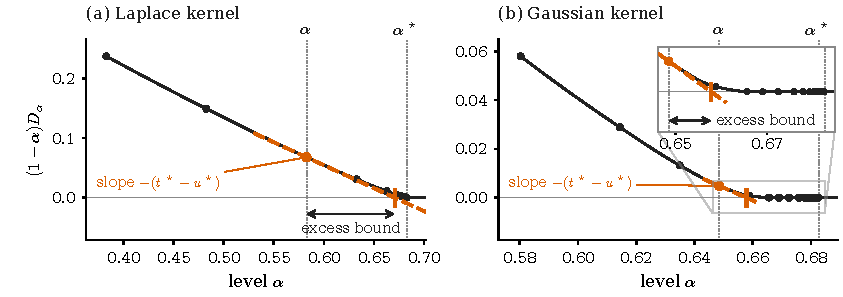
\includegraphics[width=\textwidth]{figs_aos/fig_excess_aos.pdf}
\caption{The rescaled path $(1-\alpha)D_\alpha$ for $P=N(1,1)$ and $Q=N(-1,1)$, whose total variation is
$\alpha^\star=2\Phi(1)-1\approx\fxAlphaStar$, with the Laplace kernel (a) and the Gaussian kernel (b), both with
$\sigma=1$ (dots: computed levels; line: monotone interpolation). At $\alpha=\fxLevelLap$ in (a) and
$\alpha=\fxLevelGauss$ in (b) the dashed line of slope $-(t^\star-u^\star)$ supports the path; the excess of the
population ramp over $\alpha$ is at least the distance (arrow) from $\alpha$ to the zero of the line (tick), by
Proposition~\ref{prop:excess}, and the inset of (b) enlarges the region near $\alpha^\star$. That distance is a fraction
$\fxFracLap$ of $\alpha^\star-\alpha$ for the Laplace kernel and $\fxFracGauss$ for the Gaussian kernel at this level,
closer to $\alpha^\star$. The Gaussian fraction, $\fxFracGaussAtLap$ at $\alpha=\fxLevelGaussAtLap$, falls toward zero
as $\alpha\uparrow\alpha^\star$, where its path is flatter than every power.}
\label{fig:excess}
\end{figure}

\subsection{Touching contaminations, and why the margin is pessimistic}
\label{sec:touching}

Under the hypotheses of Proposition~\ref{prop:newsobolev}, Theorem~\ref{thm:loratemain} guarantees at least the rate
$(n\wedge m)^{-2/(2s+3)}$, $(n\wedge m)^{-2/5}$ for the Laplace kernel, which Theorem~\ref{thm:laplacerate} improves to
$(n\wedge m)^{-1/2}$, up to powers of $\log(n\vee m)$, under one more condition, for samples of comparable size. Under those of Proposition~\ref{prop:newgauss} the margin
guarantees at least the logarithmic rate $c/\log(n\wedge m)$ for every $c>\pi^2\sigma^2\ell_0/4$, on grids with at
most $(n\wedge m)^b$ levels for a fixed $b$ (Proposition~\ref{prop:newrates} of the supplement), in both cases up to the
mesh. For the split-sample bound we prove no converse. For the analytic baseline run with the larger threshold
$\tau^{\mathrm S}$ the margin rate cannot be improved for Sobolev kernels, and with the Gaussian kernel its error is
not $O((n\wedge m)^{-a})$ for any $a>0$ (Proposition~\ref{prop:newconverse} of the supplement); for
$\tau^{\mathrm P}$ no converse is known.

The margin is pessimistic. Theorem~\ref{thm:loratemain} bounds the excess $\E_P\rp-\E_Q\rp-\alpha$ of the population
ramp from below by $D_\alpha/(\beta\Delta_\phi)$ (Lemma~\ref{lem:popramp} of the supplement), replacing the gap
$t^\star-u^\star$ between its cut points by its largest value $\Delta_\phi$. The gap is a slope of the rescaled
path $(1-\alpha)D_\alpha$, the distance between the parts of mass $1-\alpha$ that the trimmings keep, which is convex in
$\alpha$ (Lemma~\ref{lem:pathconvex} of the supplement). The line through the point of the rescaled path at $\alpha$
with slope $-(t^\star-u^\star)$ supports it, and the excess of the ramp is at least the distance from $\alpha$ to the
zero of this line (Proposition~\ref{prop:excess}, Figure~\ref{fig:excess}). When the path lies between two multiples of one power of
$\alpha^\star-\alpha$, this distance is a fixed fraction of $\alpha^\star-\alpha$.

\begin{proposition}[Excess of the population ramp]
\label{prop:excess}
Let Assumption~\ref{ass:regularity} hold, let $0<\alpha^\star<1$, let $\alpha<\alpha^\star$, let $f^\star$ be the
direction of the population witness, $t^\star$ the smallest $(1-\alpha)$-quantile of $f^\star(X)$ and $u^\star$ the
largest $\alpha$-quantile of $f^\star(Y)$, so that $t^\star-u^\star\ge D_\alpha>0$ (Lemma~\ref{lem:popramp} of the
supplement), and let $\rp^\star$ be the ramp of $f^\star$ between $u^\star$ and $t^\star$. Then:
\begin{enumerate}[label=(\roman*),leftmargin=*]
\item $\E_P\rp^\star-\E_Q\rp^\star-\alpha\ge(1-\alpha)D_\alpha/(t^\star-u^\star)$, and
$(1-\alpha')D_{\alpha'}\ge(1-\alpha)D_\alpha-(t^\star-u^\star)(\alpha'-\alpha)$ for every $\alpha'\in[0,1)$;
\item if $c_1\epsilon^\gamma\le D_{\alpha^\star-\epsilon}\le c_2\epsilon^\gamma$ for $0<\epsilon\le\epsilon_0\le\alpha^\star$, then
at $\alpha=\alpha^\star-\epsilon$ with $\epsilon\le\epsilon_0/2$ the excess in (i) is at least
$(1-\alpha^\star)c_1\epsilon/(2^\gamma c_2)$, and this holds under the hypotheses of Proposition~\ref{prop:newsobolev};
\item for the Laplace kernel $e^{-|x-y|/\sigma}$ on $\R$, $u^\star\le f^\star\le t^\star$ on $\R$ and the first
inequality of (i) is an equality.
\end{enumerate}
\end{proposition}

On the line, by part (iii), the Laplace witness is already clipped at its cut points, and so is the witness fitted on
the data, whose ramp maximizes the ratio of empirical excess to RKHS norm over functions of oscillation at most one
(Lemma~\ref{lem:lapclip} of the supplement). Comparing this ratio with the population path at two levels shows that the
fitted ramp keeps a fixed fraction of the excess of the population ramp (Proposition~\ref{prop:lapfitted}).

\begin{theorem}[Near-parametric rate with the Laplace kernel]
\label{thm:laplacerate}
Let $P,Q$ satisfy the hypotheses of Proposition~\ref{prop:newsobolev} on the laws, let $n\wedge m\ge10$, and compute
$\widehat\alpha$ as in Theorem~\ref{thm:loratemain}, on a grid of $J$ levels in $(0,1)$ with mesh $\Delta_{\mathcal G}$
below $\alpha^\star$, with the kernel $e^{-|x-y|/\sigma}$, $\sigma>0$ fixed in advance, an exact minimizer of
\eqref{eq:qp} at each level, and, in place of the one-rank tolerance \eqref{eq:cutrank}, cut points that are genuine
empirical quantiles of the witness values, computed with or without each point's own term in \eqref{eq:witness}. Let
$\eta\in(0,1)$, $L_\delta=\log(1/\delta)$, $L_{n,m}=\log\{(n\vee m)/\eta\}$ and
$B_{n,m}=v_{\min}^{-2}\{L_\delta^{1/2}+(\log(2J/\eta))^{1/2}\}(n\wedge m)^{-1/2}$.
\begin{enumerate}[label=(\roman*),leftmargin=*]
\item If for some $r_\ast\in(0,1]$ and $c_\ast>0$
\begin{equation}
|p(x)-q(x)|\ \ge\ c_\ast\min(r_\ast,|x-x_0|)\,\{p(x)+q(x)\}\qquad\text{for almost every }x,
\label{eq:condR}
\end{equation}
then with probability at least $1-\delta-\eta$,
\[
\alpha^\star-\Delta_{\mathcal G}-O\big(L_{n,m}^{3/4}(n\wedge m)^{-1/2}+B_{n,m}\big)\ \le\ \widehat\alpha\
\le\ \alpha^\star .
\]
\item If instead $(P+Q)(\{x:|x-x_0|>t\})\le C'e^{-t/C'}$ for all $t>0$, the same holds with
$L_{n,m}^{2/3}(n\wedge m)^{-4/9}$ in place of $L_{n,m}^{3/4}(n\wedge m)^{-1/2}$.
\end{enumerate}
The constant in the $O$ depends only on $\sigma$ and on the pair, as stated in Theorem~\ref{thm:laplaceconst} of the
supplement.
\end{theorem}

Under these hypotheses $\TV(P,Q)=F_Q(x_0)-F_P(x_0)$ is a one-sided Kolmogorov distance, which the one-sided
Kolmogorov--Smirnov statistic bounds from below at the rate $(n\wedge m)^{-1/2}$, with no condition on the likelihood
ratio and no logarithmic factor. The interest of the theorem is that a kernel bound that does not sort the
data, and returns the set, attains this rate up to logarithmic factors, which the margin does not see; it is no reason
to prefer the method on the line. Condition \eqref{eq:condR} asks that $p/q$ stay away from one off every neighborhood of $x_0$, so it excludes
contaminations local to a common core, with $p=q>0$ on an interval, where only part (ii) applies. No multivariate theorem
singles out the Laplace kernel in $\R^d$, where its choice rests on this one-dimensional theory and on its power against
differences of high frequency, seen on a one-dimensional oscillating density (Section~\ref{sec:numharder}). Section~\ref{sec:laplaceproof} of the supplement discusses
the exact minimizers the theorem needs, its constants, whose uniformity over a class is open, and a simulation.

\section{The trimming}
\label{sec:trimming}

Once we know that at least a fraction $\widehat\alpha$ of each population has no counterpart in the other, the next
question is which observations these are. By Proposition~\ref{prop:bangbang} the minimizer of \eqref{eq:qp} answers it
with a pair of trimmed samples, which keep at full weight the observations on one side of a cut of the witness and split
weight among those at the cut. They converge, at a fixed level to the best trimming at that level and at the estimated
level to the common core. The rate we prove at a fixed level assumes a witness with a density at the cut, condition
\eqref{eq:qdens} below, as for the Gaussian kernel (Remark~\ref{rem:qdens} of the supplement). With the Laplace kernel
on the line the population witness equals its cut on a set of $P$-mass at least $\alpha$ (Section~\ref{sec:excessproofs}
of the supplement), so \eqref{eq:qdens} fails at every level, Theorem~\ref{cor:trimrate} does not apply, and the
trimming is decided among tied observations; Section~\ref{sec:trimest}, in MMD and without a rate, covers every kernel
of Assumption~\ref{ass:regularity}.

\subsection{A parametric rate at a fixed level}

Fix $\alpha$ with $D=D_\alpha(P,Q)>0$, which under (A3) means $\alpha<\alpha^\star$, let $d^\star$ be the population
witness of Section~\ref{sec:statistic}, with direction $f^\star=d^\star/D$, and let $t_\alpha$ be a $(1-\alpha)$-quantile
of $d^\star(X)$ under $P$. The population version of Proposition~\ref{prop:bangbang} holds: every optimal trimming
density of $P$ has the threshold form (Lemma~\ref{lem:popthreshold} of the supplement)
\begin{equation}
g^\star=\beta\,\mathbf 1\{d^\star<t_\alpha\}+\vartheta\,\mathbf 1\{d^\star=t_\alpha\},
\qquad 0\le\vartheta\le\beta\ \text{a function with}\ \E_P[g^\star]=1 .
\label{eq:popdensity}
\end{equation}
The observations that an optimal trimming keeps at full weight form the \emph{kept sets}
\[
A^\star\coloneqq\{x:\ d^\star(x)<t_\alpha\}
\qquad\text{and}\qquad
\widehat A_n\coloneqq\{x:\ \widehat d(x)<\widehat t_n\},
\]
population and empirical, whose symmetric difference $\widehat A_n\triangle A^\star$ measures the error, and we let
$\widehat g_n$ be the density \eqref{eq:popdensity} with $(\widehat d,\widehat t_n)$ in place of $(d^\star,t_\alpha)$
and any tie function $0\le\widehat\vartheta\le\beta$, a rule that need not integrate to one under $P$. Level sets are
stable where the witness has a density at the cut, which we ask at both cuts:
\begin{gather}
\tag{Q}\label{eq:qdens}
\parbox[t]{0.84\textwidth}{\raggedright the law of $d^\star(X)$ under $P$ has, on $[t_\alpha-r_Q,t_\alpha+r_Q]$ for some
$r_Q>0$, a density with values in $[c_f,C_f]$, where $0<c_f\le C_f<\infty$;}\\[4pt]
\tag{Q$'$}\label{eq:qdensY}
\parbox[t]{0.84\textwidth}{\raggedright the law of $d^\star(Y)$ under $Q$ has, on $[u_\alpha-r_Q,u_\alpha+r_Q]$, a
density at least $c'_f>0$, where $u_\alpha$ is an $\alpha$-quantile of $d^\star(Y)$.}
\end{gather}
Condition \eqref{eq:qdens} is the classical quantile-density condition for the cut of the $X$ sample, and
\eqref{eq:qdensY} its lower half for the cut of the $Y$ sample. Laws with finite support, such as those of
Example~\ref{ex:separated} with finitely supported $R$, $P_0$, $Q_0$, violate \eqref{eq:qdens}, so the margin does not imply the density conditions. The rate comes from a localization argument of the kind behind rates for M-estimators
\citep[Theorem~3.2.5]{vandervaart1996weak}: the separation of Section~\ref{sec:ramp} falls quadratically away from its
maximizer $f^\star$, while its fluctuation grows linearly in the distance to $f^\star$, times $(n\wedge m)^{-1/2}$.

\begin{theorem}[A parametric rate for the witness and the kept set]
\label{cor:trimrate}
Let (A1) and (A2) of Assumption~\ref{ass:regularity} hold, fix $\alpha\in(0,1)$ with $D=D_\alpha(P,Q)>0$, and suppose
\eqref{eq:qdens} and \eqref{eq:qdensY}. Put $V_\alpha=\kappa\beta+[\beta/\min(c_f,c'_f)]^{1/2}$ and
$W_\alpha=C_f(\kappa V_\alpha+c_f^{-1})$. Then, with $(P,Q,k,\alpha)$ fixed and $n\wedge m\to\infty$,
\begin{gather*}
\big\|\widehat f-f^\star\big\|_\Hh=O_\Pp\Big(\frac{V_\alpha}{D\sqrt{n\wedge m}}\Big),
\qquad
\|\widehat d-d^\star\|_\Hh=O_\Pp\Big(\frac{V_\alpha}{\sqrt{n\wedge m}}\Big),\\
P(\widehat A_n\triangle A^\star)=O_\Pp\Big(\frac{W_\alpha}{\sqrt{n\wedge m}}\Big),
\qquad
\frac1\beta\int|\widehat g_n-g^\star|\,dP=O_\Pp\Big(\frac{W_\alpha}{\sqrt{n\wedge m}}\Big),
\end{gather*}
with constants in the $O_\Pp$ that depend only on the probability level.
\end{theorem}

The rate is that of a sample quantile, free of the dimension of $\mathcal X$, because the witness converges in $\Hh$,
as a mean of feature vectors, and the kept set inherits its rate through the density at the cut. As
$\alpha\uparrow\alpha^\star$ the bound on the direction grows like $1/D$, and the sample size from which the bounds hold,
not explicit (Section~\ref{app:trimming} of the supplement states what it depends on), grows as $D$ vanishes. The kept set then has in general no limit, because the common
core keeps only a fraction of $P$ on the set $\{0<q<p\}$, and an indicator of a set cannot converge to such a
fractional weight. With the Wasserstein distance, optimal trimmings are consistent and computable
\citep{alvarez2011incomplete,agullo2018trimming}, and rates are known only toward a known target
\citep{delbarrio2013rates}.

\subsection{The trimming at the estimated level}
\label{sec:trimest}

In practice the trimming is read at a data-driven level, the lower bound $\widehat\alpha$, where
Theorem~\ref{cor:trimrate} does not apply: its level is fixed in advance, and its bounds degrade as $D_\alpha(P,Q)$
vanishes near $\alpha^\star$. There the trimmed sample still converges as a measure. The common core $R^\star$ is the unique common
trimming at $\alpha^\star$, and
\[
\Omega(\epsilon)=\sup\big\{\|a-\mu_{R^\star}\|_\Hh:\ a\in\mathcal C_{\alpha^\star}(P),\
\dist\big(a,\mathcal C_{\alpha^\star}(Q)\big)\le\epsilon\big\}
\]
is a modulus of the contact of the two regions at $\alpha^\star$.

\begin{proposition}[The trimmed sample at the data-driven level]
\label{prop:alphahat}
Let Assumption~\ref{ass:regularity} hold and let $0<\alpha^\star<1$. Then $\Omega(\epsilon)\to0$ as
$\epsilon\downarrow0$. Fix $\delta'\in(0,1)$ and put $r_n=\kappa(1-\alpha^\star)^{-1}[4n^{-1/2}+(2\log(2/\delta')/n)^{1/2}]$,
and $r_m$ likewise. There is an event $E$ of probability at least $1-2\delta'$, not depending on the level, on which for
every level $\tilde\alpha\le\alpha^\star$, possibly chosen from the data, and every $(w,v)\in\mathcal T_{\tilde\alpha}$,
\[
\MMD\big(P_n^w,R^\star\big)\le r_n+\Omega\big(\widehat D_{\tilde\alpha}+r_n+r_m\big).
\]
The same holds for the second sample, with $P$ and $Q$ exchanged.
\end{proposition}

On $E$ each empirical region is within $r_n$, respectively $r_m$, of its population counterpart, at all levels up to
$\alpha^\star$ at once, by \eqref{eq:hausdorff}. The bound covers the trimming read at $\widehat\alpha$ or at any other
valid lower bound. It carries no rate unless $\Omega$ is known, and it places the reweighted sample near the common core
without saying which observations are kept.

\begin{corollary}[The trimmed sample at the lower bound]
\label{cor:alphalo}
Let Assumption~\ref{ass:regularity} hold, let $0<\alpha^\star<1$, and compute $\widehat\alpha$ at level
$\delta$ as in Proposition~\ref{prop:loconsistency}, on grids fixed in advance whose mesh tends to zero, with
$\log J=o(n\wedge m)$. Then for every $\epsilon>0$ and $\delta'\in(0,1)$, for all $n,m$ large enough, with probability
at least $1-\delta-\delta'$ every $(w,v)\in\mathcal T_{\widehat\alpha}$ has
$\MMD(P_n^w,R^\star)\le\epsilon$ and $\MMD(Q_m^v,R^\star)\le\epsilon$.
\end{corollary}

By Lemma~\ref{lem:pathconvex}(ii) of the supplement the path falls to zero at most linearly, so a consistent
$\widehat\alpha$ has a small trimmed distance whatever the laws and no margin is needed. The proof uses
$\widehat\alpha$ only through its validity and its consistency, so the level may come from a bound computed with
another kernel than the one that trims, as in Section~\ref{sec:appcohort}.

\section{Numerical results}
\label{sec:numerical}

The theory says that the split-sample bound is valid at every sample size, but not how large the sample must be for
it to be useful. We measure this on simulated data whose total variation is known, and on two public data sets,
where the trimming at the certified level also gives a cohort.

\subsection{Simulations}
\label{sec:numharder}

Every design follows the contamination model \eqref{eq:contam}, with a common component of weight $1-a$ shared by $P$
and $Q$ and two design components $P_0$ and $Q_0$ of weight $a$, so that
$\TV(P,Q)=a\,\TV(P_0,Q_0)$ is known in closed form; $\alpha^\star=0.2$ unless a design says otherwise. The $\allNdesigns$ designs, listed in Table~\ref{tab:hardern80} and described in
Table~\ref{tab:harderdesigns} of the supplement, vary one feature at a time: where the contamination sits, the
dimension, how the signal is spread, its size, the type of data, and how smooth the difference of the densities is. In
the overlap and shift designs $P_0$ and $Q_0$ are $N(\pm\mu,I)$ on a $N(0,I)$ core, with $\mu$ along one
coordinate, along two or spread over all of them, so that $\{p>q\}$ is a half-space; the correlation flip changes the
sign of one correlation, the $t_3$ design the scale of one coordinate of a $t_3$ law, and the curves add or subtract a
bump to Brownian paths. The oscillating densities are those of Section~\ref{sec:upper}, which a fixed kernel sees less
and less as their frequency $\nu$ grows. One design is shaped on the RHC data of Section~\ref{sec:data}: it keeps the $\rrRhcNcovPaper$
covariates stored as numbers, takes a smoothed resample of the patients as the common component, and places $P_0$ and $Q_0$
in boxes at $\pm\rgSep$ pooled standard deviations in four coordinates.

Four methods certify a level of $\TV$. The split-sample bound $\widehat\alpha$ is Algorithm~\ref{alg:split} of the
supplement with the Laplace kernel, whose bandwidth is the median distance among the points each witness is fitted on.
The analytic baseline $\widehat\alpha_{\mathrm{an}}$ uses the threshold of Theorem~\ref{thm:plugin} and a Gaussian
kernel with its bandwidth fixed on a separate pilot draw of $1{,}000$ points from each law ($400$ and $2{,}000$ for
mixed types), not counted in $n$ or $m$. The other two run the same betting test on the labels of a
classifier, gradient boosting (GBM) or logistic regression \citep{pedregosa2011sklearn}, trained on the first half of
each sample as in \citet{naf2022hplb}. For reference we add two tests of $P=Q$, the permutation test of the MMD, with
the Gaussian kernel at the pilot bandwidth, and MMDAgg \citep{schrab2023aggregated}; they detect a difference but
certify nothing about its size. All methods see the same replicates, $\mnRepsPerSize$ per design and size, with $n=m$
doubling from $\harderNmin$ to $\harderNmax$ (mixed types: $n$ up to $400$, with $m=5n$). The four that certify are also
run at $\fourdigits{\harderNtwo}$ in the two designs of Table~\ref{tab:harderdesigns} that list it and, in every
design, at sizes doubling from $\fourdigits{\harderNtwo}$ to $\harderNcap$ until their power against $H_{0,0}$ reaches
$0.8$. The two tests of $P=Q$ are also run at $\fourdigits{\harderNtwo}$ on the narrow bump. The four that certify
test $H_{0,\alpha}$ at the levels $\alpha=j\alpha^\star/8$, $j=0,\dots,10$, with $\delta=0.05$.

We first check validity: a test may reject a true null, and the bound exceed $\alpha^\star$, with probability at most
$\delta$. At the level $\alpha=\alpha^\star$ the null $H_{0,\alpha^\star}$ holds, as $\TV(P,Q)$ is
exactly $\alpha^\star$: there, at $n=m=800$ (mixed types: $n=400$, $m=5n$), the betting test on the Laplace ramp
rejected $\mnBdTotal$ times in $\mnBdReps$ replicates in all, and at most $\mnBdMax$ in any one design. When $P=Q$, a
rejection of $H_{0,0}$ falsely claims a difference: on four designs in which both samples come from the same law,
over $\mnNullCells$ combinations of design and sample size, the same test rejected in $\mnNullPct\%$ of the replicates,
and at most $\mnNullMax$ in one combination. The analytic test never rejected in either case. For no method and no
combination does a binomial test at level $0.01$ find more rejections than $\delta$ allows, and in every design the
split-sample bound exceeded $\alpha^\star$ in at most a fraction $\mnAloGtMax$ of the replicates, well within the
$\delta$ that Corollary~\ref{cor:lower} allows (Section~\ref{app:experiments} of the supplement).

\begin{table}[t]
\centering
\footnotesize
\setlength{\tabcolsep}{5pt}
% Generated by scripts/aos_main_tables.py -- do not edit. Sample size n = m (mixed: n, m = 5n) for power 0.8 against H_{0,0} (first size with power >= 0.8, log-linear interpolation, two significant digits). Laplace ramp: results/aos/main (alpha = 0, Laplace kernel, all stored sizes and the alpha = 0 extension); analytic: tau = min{tau^P, tau^A} on the stored statistics; GBM, logistic: stored study; perm. MMD, MMDAgg: results/aos/baselines. Bold: smallest of the four tests that certify a level; italic: smaller of the two tests of P = Q.
\begin{tabular}{lccccccc}
\toprule
design & $\alpha^\star$ & $\widehat\alpha$ & $\widehat\alpha_{\mathrm{an}}$ & GBM & logistic & perm. & MMDAgg \\
 &  &  &  & + betting & + betting & MMD &  \\
\midrule
RHC-shaped, $d=33$ & $0.2$ & $\mathbf{{\le}100}$ & $450$ & $250$ & $230$ & $\mathit{{\le}100}$ & $\mathit{{\le}100}$ \\
overlap, $d=2$ & $0.1$ & $\mathbf{670}$ & $2{,}600$ & $5{,}100$ & $1{,}100$ & $\mathit{340}$ & $400$ \\
overlap, $d=2$ & $0.2$ & $\mathbf{160}$ & $620$ & $720$ & $280$ & $\mathit{{\le}100}$ & $\mathit{{\le}100}$ \\
overlap, $d=10$ & $0.1$ & $\mathbf{890}$ & $11{,}000$ & $4{,}900$ & $1{,}300$ & $\mathit{510}$ & $670$ \\
overlap, $d=10$ & $0.2$ & $\mathbf{180}$ & $1{,}500$ & $690$ & $320$ & $\mathit{{\le}100}$ & $130$ \\
dense shift, $d=20$ & $0.2$ & $\mathbf{210}$ & $2{,}800$ & $650$ & $360$ & $\mathit{120}$ & $150$ \\
dense shift, $d=50$ & $0.2$ & $\mathbf{300}$ & $5{,}800$ & $730$ & $500$ & $\mathit{160}$ & $190$ \\
dense shift, $d=100$ & $0.2$ & $\mathbf{380}$ & $11{,}000$ & $1{,}000$ & $690$ & $\mathit{210}$ & $240$ \\
sparse shift, $d=50$ & $0.2$ & $\mathbf{300}$ & $5{,}800$ & $660$ & $530$ & $\mathit{160}$ & $180$ \\
correlation flip, $d=50$ & $0.2$ & ${>}12{,}800$ & ${>}12{,}800$ & $\mathbf{5{,}200}$ & ${>}12{,}800$ & ${>}800$ & ${>}800$ \\
small contamination, $d=2$ & $0.05$ & $\mathbf{900}$ & $5{,}100$ & $5{,}500$ & $3{,}500$ & $600$ & $\mathit{500}$ \\
mixed types, $m=5n$ & $0.2$ & $\mathbf{140}$ & $660$ & $390$ & $170$ & $\mathit{{\le}100}$ & $\mathit{{\le}100}$ \\
$t_3$ tails, $d=5$ & $0.2$ & $\mathbf{320}$ & $2{,}800$ & $1{,}000$ & ${>}12{,}800$ & $\mathit{220}$ & $300$ \\
curves, wide bump & $0.2$ & $\mathbf{270}$ & $1{,}300$ & $690$ & $390$ & $\mathit{180}$ & $240$ \\
curves, narrow bump & $0.2$ & $1{,}200$ & $11{,}000$ & $1{,}100$ & $\mathbf{420}$ & $1{,}200$ & $\mathit{1{,}000}$ \\
oscillating, $\nu=1$ & $0.5$ & $\mathbf{{\le}100}$ & $\mathbf{{\le}100}$ & $\mathbf{{\le}100}$ & $\mathbf{{\le}100}$ & $\mathit{{\le}100}$ & $\mathit{{\le}100}$ \\
oscillating, $\nu=4$ & $0.5$ & $230$ & $2{,}600$ & $\mathbf{150}$ & $10{,}000$ & $580$ & $\mathit{{\le}100}$ \\
oscillating, $\nu=16$ & $0.5$ & $2{,}900$ & ${>}12{,}800$ & $\mathbf{290}$ & ${>}12{,}800$ & ${>}800$ & ${>}800$ \\
oscillating, $\nu=64$ & $0.5$ & ${>}12{,}800$ & ${>}12{,}800$ & $\mathbf{720}$ & ${>}12{,}800$ & ${>}800$ & ${>}800$ \\
\bottomrule
\end{tabular}

\caption{Sample size $n=m$ (mixed types: $n$, with $m=5n$) at which each method reaches power $0.8$ against
$H_{0,0}$ at $\delta=0.05$, from $\mnRepsPerSize$ replicates per size, interpolated between the two sizes that bracket
$0.8$ and rounded to two significant digits; ${\le}\mnNmin$, ${>}\mnNcap$: reached at the smallest size, not reached
at the largest. Bold: the smallest among the four tests that certify a level of $\TV$; italic: the smaller of the last
two, which test $P=Q$ only. $\widehat\alpha$: the betting test of Theorem~\ref{thm:betting} on the Laplace ramp;
$\widehat\alpha_{\mathrm{an}}$: the analytic test \eqref{eq:test} with the Gaussian kernel; GBM, logistic: the betting test on the labels of
gradient boosting and logistic regression trained once on half of the data, a handicap removed in Figure~\ref{fig:recovery}; perm.\ MMD: permutation test
with the Gaussian kernel at the pilot bandwidth of the analytic test and $\abPermB$ relabelings; MMDAgg: the test of
\citet{schrab2023aggregated}; the last two were run up to $n=800$ ($\fourdigits{\harderNtwo}$ on the narrow bump), so
${>}800$ means not reached there. The analytic and permutation tests take their bandwidth from a separate pilot draw,
not counted in $n$ (Section~\ref{sec:numharder}).}
\label{tab:hardern80}
\end{table}

The next question is how many observations each method needs to detect the contamination, that is, to reject
$H_{0,0}$ with power $0.8$ (Table~\ref{tab:hardern80}). Against classifiers trained once on half of the data, the
split-sample bound needs the fewest observations among the methods that certify a level of $\TV$ in
$\mnNeightyRampBest$ of the $\allNdesigns$ designs, alone in $\mnNeightyRampBestAlone$. Gradient boosting needs fewer
where the kernel at its bandwidth barely sees the difference, on the correlation flip, whose population MMD is about
zero, and on the oscillating densities with $\nu\ge4$, and both classifiers need fewer on the narrow bump. Refitted on
the batches of the ramp, the best of the classifiers, default or tuned, has more power at $n=m=800$ than the
split-sample bound in $\mnPowBestClfAboveLap$ designs and less in $\mnPowLapAboveBestClf$
(Section~\ref{sec:baselines} of the supplement). The analytic baseline needs $\mnAnaOverRampLo$ to $\mnAnaOverRampHi$ times
as many observations as the split-sample bound (median $\mnAnaOverRampMed$, over the designs where both sizes are
interpolated), the price of a threshold that holds for every pair in the null. It fires close to where the design rule
\eqref{eq:samplesize} predicts, at $\mnTauFireRatioLo$ to $\mnTauFireRatioHi$ times the size at which $\tau(0)$ meets
the population MMD.

Detecting a difference without certifying its size takes fewer observations. The permutation test of the MMD is the
fastest of all methods, or tied for fastest, in $\mnNeightyPermBest$ designs, and where both sizes are interpolated the
split-sample bound needs $\mnNeightyRampOverPermLo$ to $\mnNeightyRampOverPermHi$ times as many observations (median
$\mnNeightyRampOverPermMed$). The split-sample bound spends a quarter of each sample on fitting alone and pays for
betting, while the permutation test also takes its bandwidth from the pilot draw; the ratio falls below one only on the
oscillating density with $\nu=4$.

\begin{figure}[t]
\centering
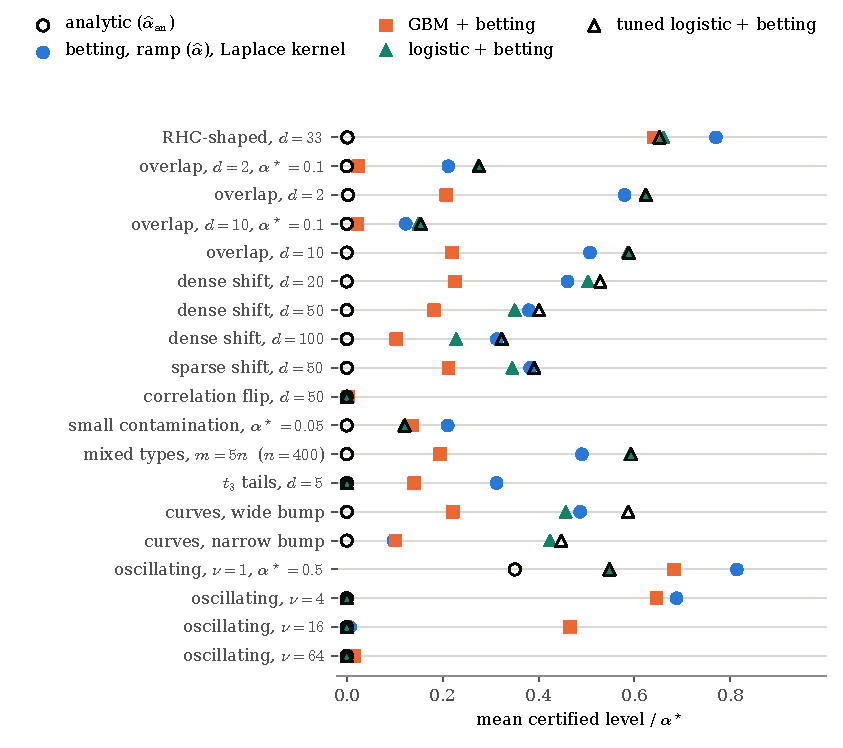
\includegraphics[width=\textwidth]{figs_aos/fig_recovery_main.pdf}
\caption{How much of $\alpha^\star$ each lower bound recovers at $n=m=800$ (mixed types: $n=400$, $m=5n$): the mean
over $\mnRecReps$ replicates of the largest level $j\alpha^\star/8$ it certifies divided by $\alpha^\star$, with $0$
when it certifies none, on a grid that uses the known $\alpha^\star$; $\alpha^\star=0.2$ unless shown, $\delta=0.05$;
classifiers: labels bet on the batches of the ramp.}
\label{fig:recovery}
\end{figure}

Detection certifies only the first level of the grid, and the bound is meant to certify as much of $\alpha^\star$ as
it can. We measure this by the recovery, the mean over replicates of the largest certified level divided by
$\alpha^\star$. The grid $j\alpha^\star/8$ uses the known $\alpha^\star$ only to express the levels as fractions of
it, and its largest level below $\alpha^\star$ is $7\alpha^\star/8$, so a valid bound recovers at most about
$\rcGridCeiling$. At $n=m=800$ the split-sample bound recovers a median $\mnRecRampMedian$ and a mean
$\mnRecRampMean$ over the designs, at most $\mnRecRampMax$, and $\mnRecRhcRamp$ on the RHC-shaped design
(Figure~\ref{fig:recovery}), while the
analytic baseline recovers a visible fraction only on the oscillating density with $\nu=1$, $\mnRecAnalyticMax$.

No bound recovers all of $\alpha^\star$ at this size. Near $\alpha^\star$ the excess of every function over $\alpha$ is
small, and a bet needs many pairs to detect a small excess: even the oracle that runs the same test on the better of
$\mathbf 1\{p>q\}$ and a level set of $p/q$ recovers a median $\rcOracleMedEightHundred$. Relative to this oracle,
with $\rcReps$ replicates per size below $800$, the recovery of the split-sample bound has median $\rcRatioMedHundred$, $\rcRatioMedTwoHundred$, $\rcRatioMedFourHundred$
and $\rcRatioMedEightHundred$ at $n=m=100$, $200$, $400$ and $800$, and the ratio is larger at $800$ than at $100$ in
$\rcRatioGrows$ of the $\rcRatioGrowsOf$ designs; in the other two the bound certifies almost nothing at any size
(Figure~\ref{fig:recoverycurves} of the supplement shows the curves).

Tuned classifiers can recover more than the split-sample bound where their model fits $\{p>q\}$. Refitted on the
batches of the ramp, unlike in Table~\ref{tab:hardern80}, so that all methods bet on the same observations, tuned
logistic regression recovers more than the bound in $\wtllosses{\mnWtlRecLogitTuned}$ designs and less in
$\wtlwins{\mnWtlRecLogitTuned}$, differences within two paired standard errors counting as ties, mostly more where
$\{p>q\}$ is a half-space, and tuned gradient boosting recovers more, at two decimals, on several designs, among them
the $t_3$ tails and the oscillating densities with $\nu\le16$; with default settings, the bound's mean recovery is
higher than that of the better of the two classifiers in $\mnRampAboveBestMatched$ of the $\allNdesigns$ designs and
lower in the others (Section~\ref{sec:baselines} of the supplement).
We keep the ramp as the default because it needs no tuning beyond the median-distance bandwidth, the rates of Section~\ref{sec:rates} are proved for it, and the program
that fits it also returns the trimming of Section~\ref{sec:trimming}. Validity does not depend on this choice: an
analyst who trusts a classifier on their data can bet on its labels instead (Section~\ref{sec:betting}).

In these designs the gain over an untrimmed witness comes mostly from where the witness is cut. The Gaussian witness
fitted once at $\alpha=0$, with no quadratic program, recovers a median $\abRecMedRampZero$ when cut at $\alpha=0$ and
$\abRecMedRampZeroCut$ when cut at the quantiles of the tested level, and the witness refitted at each level
$\abRecMedRamp$. At two paired standard errors refitting recovers more than the witness fitted at $\alpha=0$ and cut
at the tested level in $\wtlwins{\abWtlRecRampZeroCut}$ designs, as much in $\wtlties{\abWtlRecRampZeroCut}$ and less
in $\wtllosses{\abWtlRecRampZeroCut}$, and, at two decimals, that witness recovers more than the Laplace split-sample
bound in $\dvZeroCutAboveLap$ designs and less in $\dvZeroCutBelowLap$. Refitting gains on the $t_3$ tails, on both bumps and on
the oscillating density with $\nu=1$, and it is what consistency requires in general: a witness fitted at $\alpha=0$
can stop short of $\alpha^\star$ (Sections~\ref{sec:lower} and~\ref{sec:alphazero}).

The theory that favors the Laplace kernel holds on the line. Over the $\allNdesigns$ designs the Laplace kernel
recovers more than the Gaussian kernel in $\mnLapGaussWins$, $\mnLapGaussWinsLine$ of them oscillating densities on the
line, as much in $\mnLapGaussTies$, and less in $\mnLapGaussLosses$, where it is behind by at most
$\mnLapGaussLossMax$. In the $\mnMvDesigns$ multivariate designs, where our theory says nothing about the kernel, it is
slightly behind the Gaussian kernel: it needs fewer observations to detect in $\mnNeightyLapBelowGaussMv$ of them and
more in $\mnNeightyLapAboveGaussMv$, and recovers less in $\mnLapGaussLossesMv$ and more in $\mnLapGaussWinsMv$. Its
higher median recovery, $\mnRecRampMedian$ against $\mnRecGaussMedian$, comes from one design: on the oscillating
density with $\nu=4$ the recovery rises from $\mnRecNfourGauss$ to $\mnRecNfourLap$, which alone lifts the median.
Without it the medians are $\mnRecRampMedianNoNfour$ and $\mnRecGaussMedianNoNfour$, and the means over all designs
$\mnRecRampMean$ and $\mnRecGaussMean$. We keep the Laplace kernel as the default because its witness still sees
differences of high frequency that the Gaussian witness at the same bandwidth misses, as on this one-dimensional
density.

\subsection{Real data}
\label{sec:data}

We apply the split-sample bound and the analytic baseline to two public data sets, which give four contrasts. The
Right Heart Catheterization (RHC) study \citep{connors1996rhc} is an observational study of critically ill adults in
which the treatment is a catheter placed in the right side of the heart; of its $\rhcNtotal$ patients, $\cohNX$
received a catheter. We use its $\rrRhcNcovFull$ numeric and binary baseline covariates, the binary ones coded $0/1$,
standardized (Section~\ref{sec:rdbw} of the supplement lists them). The National Health and Nutrition Examination
Survey (NHANES) \citep{nhanes2012,john2019mims}, cycles 2011--2014 pooled, provides wrist accelerometry, from which we
take curves: for each participant, the mean over the valid days of $\log(1+\mathrm{MIMS})$ in each hour of the day,
with MIMS the monitor-independent movement summary, a curve on $24$ points. As an illustration on functional data, we
compare children aged 6--11 with older adults aged 60--79, younger adults aged 20--39 with the same older adults, and
body mass index below $25$ with $30$ or above within ages 20--59, which holds age roughly fixed; we call these the
child, the adult age and the body-mass contrasts. NHANES is a multistage survey, and we ignore its weights and design,
so these bounds concern the laws of the sampling process rather than the population of the United States. The
independence the betting test needs then holds only approximately, since participants share households and sampling
units; assigning whole sampling units to the batches gives the same or higher minima, though pairs within a batch can
still share a unit (Section~\ref{sec:rdbw}).

Every reported split-sample bound uses the Laplace kernel, with the median distance on batch $0$ as bandwidth for both
witnesses, a rule that, as in the simulations, uses only fitting data. The analytic baseline uses a Gaussian kernel with its
bandwidth fixed on a $30\%$ pilot sample of each group, and is computed on the other $70\%$ only. Each contrast is
reported at $\delta=0.05$, with no correction for the three NHANES contrasts.

\begin{table}[t]
\centering
\small
\setlength{\tabcolsep}{2.3pt}
% Generated by scripts/aos_main_tables.py -- do not edit. Analytic: scripts/exp_valid_bandwidth.py --threshold aos (tau = min{tau^P, tau^A}), pilot route; split-sample: Laplace kernel, genuine quantile cut points, eight splits (results/aos/main/raw/realdata_laplace). RHC: the 45 covariates (rhc_full; --rhc-covariates full).
\begin{tabular}{lrrcccccccc}
\toprule
 & & & \multicolumn{5}{c}{analytic ($\widehat\alpha_{\mathrm{an}}$), pilot bandwidth} & & \multicolumn{2}{c}{split-sample} \\
\cmidrule(lr){4-8}\cmidrule(lr){10-11}
contrast & $n$ & $m$ & $\widehat D_0$ & $\tau(0)$ & $n_{\mathrm{fire}}$ & $\alpha_{\mathrm{last}}$ & bisection & & $\widehat\alpha$ (min) & $\widehat\alpha$ (avg.\ e-value) \\
\midrule
RHC arms & 2{,}184 & 3{,}551 & 0.122 & 0.089 & 1{,}006 & 0.00 & 0 &  & 0.35 & 0.35 \\
ages 6--11 vs.\ 60--79 & 1{,}969 & 2{,}300 & 0.457 & 0.100 & 72 & 0.30 & 0.3375 &  & 0.75 & 0.80 \\
ages 20--39 vs.\ 60--79 & 2{,}519 & 2{,}300 & 0.209 & 0.094 & 342 & 0.05 & 0.0625 &  & 0.35 & 0.40 \\
BMI ${<}25$ vs.\ ${\ge}30$ & 1{,}627 & 2{,}008 & 0.075 & 0.109 & 2{,}633 & -- & -- &  & 0.05 & 0.05 \\
\bottomrule
\end{tabular}

\caption{The two bounds on the four contrasts (the last three from NHANES), $\delta=0.05$, grid mesh $0.05$; $n,m$:
group sizes, of which the analytic baseline uses $70\%$ after a $30\%$ pilot. Analytic baseline: $\widehat D_0$ and
$\tau(0)$, its statistic and threshold at $\alpha=0$; $n_{\mathrm{fire}}$, the balanced size of \eqref{eq:samplesize};
$\alpha_{\mathrm{last}}$, the largest rejected grid level, and bisection, the largest level rejected when bisecting to
width $0.0125$ (Section~\ref{sec:alpha}), both at most the infimum \eqref{eq:alphaest}; `--': none. Split-sample
bound, Laplace kernel: the smallest bound over eight random splits and the level certified by the average of their
final wealths, each $\delta$-level for this kernel. The three NHANES statements hold jointly with probability at least
$1-3\delta$.}
\label{tab:realdata}
\end{table}

One split of the observations into the batches of Section~\ref{sec:betting} makes the bound depend on the split, so we
compute it on eight random splits and summarize them in two ways. Their minimum is a $\delta$-level bound, as it
exceeds $\alpha^\star$ only if every split does. The average rests on e-values, nonnegative statistics whose mean under
the null is at most one, as is the wealth of a betting test at any fixed time: at each level the wealths of the eight
tests at their horizon are e-values for $H_{0,\alpha}$, so by Markov's inequality their average reaches $1/\delta$
with probability at most $\delta$, whatever the dependence between the splits \citep{vovk2021evalues}. Either summary
is valid if fixed in advance, while reporting the larger of the two is guaranteed only at level $2\delta$. We report
the minimum. The average, shown in Table~\ref{tab:realdata} for comparison, certifies as much, and more on the two age
contrasts.

The minima say that more than $\mnRdChildMin$ of the distribution of daily profiles of children, and likewise of older
adults, has no counterpart in the other group, more than $\mnRdAgeMin$ for younger against older adults, and more than
$\mnRdBmiMin$ for the body-mass groups (Table~\ref{tab:realdata}). On RHC every split certifies $\mnRdRhcMin$, so more
than $\mnRdRhcMin$ of the covariate distribution of each arm has no counterpart in the other. On RHC and on the child
and adult age contrasts, $\mnRdRhcNoBet$, $\mnRdChildNoBet$ and $\mnRdAgeNoBet$ of the eight splits stop at a level
where the fitted cut points satisfy $\widehat t_b\le\widehat u_b$ in both batches, so that there is no ramp to bet on
and the bound is limited by the fitted witness rather than by the number of pairs; the others stop at a failed bet.
The minima depend on the kernel on two of the contrasts: with the Gaussian kernel they are the same on the age
contrasts, but $\mnRdRhcFullGaussMin$ on RHC, with the same $\rrRhcNcovFull$ covariates, and $\mnRdBmiGaussMin$ on body
mass (Section~\ref{sec:kernelfallback}). The analytic baseline rejects a positive grid level only on the age contrasts, $\alpha^\star>\mnPvChildLast$ and
$\alpha^\star>\mnPvAgeLast$; on body mass $\widehat D_0=\mnPvBmiDzero$ lies below $\tau(0)=\mnPvBmiTauzero$, and the
design rule asks for $\mnPvBmiFire$ observations per group. Bet on the batches of the ramp, the labels of the
classifiers of Section~\ref{sec:numharder} certify $\rrClfFullGbmHardMin$ on RHC, as the ramp does, except tuned
logistic regression, $\rrClfFullLogitTunedHardMin$, and their predicted probabilities certify between
$\rrClfFullLogitTunedSoftMin$ and $\rrClfFullGbmSoftMin$ (minima over the eight splits; Section~\ref{sec:rdbw}).

\subsection{From the contamination level to a cohort}
\label{sec:appcohort}

At the level $\alpha^\star$ itself, trimming both arms would give the common core $R^\star$, with density proportional
to $\min(p,q)$ for the covariate densities $p,q$ of the two arms. With $e$ the propensity score, the probability $e(x)$ that a patient with covariates $x$ receives the catheter
\citep{rosenbaum1983central}, $\pi$ the fraction of
catheterized patients and $\rho$ the pooled density, $\min(p,q)=\rho\min\{e/\pi,(1-e)/(1-\pi)\}$, an overlap population
in the sense of \citet{li2018balancing}, and for arms of equal size that of the matching weights of
\citet{ligreene2013matching}. As $p/q$ increases with $e$, $\alpha^\star$ is also the total variation between the laws
of $e(X)$ in the two arms. Replacing $e$ by a logistic fit and $\rho$ by the pooled sample in
$\alpha^\star=1-\int\min(p,q)$ gives $\rrPropFullPlug$ (bootstrap interval $(\rrPropFullPlugLo,\rrPropFullPlugHi)$),
an estimate that rests on the propensity model and certifies nothing (Section~\ref{sec:rdbw}). Trimming near
$\alpha^\star$ targets the patients for whom both treatments are plausible, as propensity trimming does with a model
\citep{yang2018asymptotic}, while the rules of Section~\ref{sec:intro} aim at positivity.

At the level $\alpha=\lcCohAlpha$ of the lower bound on RHC we trim both arms with the Gaussian kernel at the pooled
median distance, which Corollary~\ref{cor:alphalo} allows for any valid and consistent level, here one from the Laplace bound. The program \eqref{eq:qp} has a unique minimizer, as
the Gram matrix of the patients is positive definite. It gives positive weight to $\lcPoolKeptX$ of the $\cohNX$ catheterized patients and
$\lcPoolKeptY$ of the $\cohNY$ others, and fractional weight only to the $\lcPoolFracX$ and $\lcPoolFracY$ on which the
witness equals its cut (Proposition~\ref{prop:bangbang}(ii)), which carry fractions $\lcPoolFracMassX$ and
$\lcPoolFracMassY$ of the trimmed samples (Section~\ref{sec:rdbw}). With the Laplace kernel, whose witness on the line
is flat on the set it trims (Proposition~\ref{prop:excess}(iii)), the program at the same level leaves $\lpPoolFracX$ and $\lpPoolFracY$ patients with fractional
weight.

The cohort is a $\lcCohAlpha$-trimming of each arm. Proposition~\ref{prop:alphahat} and Corollary~\ref{cor:alphalo}
describe such trimmings for a kernel fixed in advance, while here the bandwidth is the pooled median. The cohort leaves the
largest standardized difference of the $\rrRhcNcovFull$ covariates at $\lcTrimSMD$, below the usual threshold $0.1$.
A trimming balances only what it sees. In a separate run on the $\rrRhcNcovPaper$ covariates stored as numbers, the
Laplace trimming at the level $\rrCohPaperAlpha$ of the bound on them leaves $\rrCohPaperOmitSmdAbove$ of the other $\rrRhcNcovAdded$ above $0.1$, against
$\rrAddedSmdAbove$ before trimming. Matching and overlap weights balance more tightly but need a propensity model,
whose covariates the overlap weights balance exactly by construction (Table~\ref{tab:cohort}). The $30$-day mortality
difference, $\lcUnwRD$ in the raw arms, is $\lcTrimRD$ under the trimming, with interval $(\lcTrimRDlo,\lcTrimRDhi)$,
and up to $\lcRDmax$ under the other weightings, with overlapping intervals. These are illustrations, not causal
estimates: they would estimate effects only under no unmeasured confounding, and the intervals ignore the estimation of
the weights. As $\lcCohAlpha$ is a lower bound on $\alpha^\star$, the trimming approaches the common core only as the
level approaches $\alpha^\star$ (Corollary~\ref{cor:alphalo}), and the level should be reported with any effect
estimated on the cohort.

\section{Final comments}
\label{sec:discussion}

We have bounded $\alpha^\star=\TV(P,Q)$ from below by following the embeddings of all trimmings of the two laws
rather than one optimal trimming. They form convex regions that meet exactly at $\alpha^\star$ and fluctuate like
sample means, which gives guarantees at every sample size on any sample space with a kernel as in
Assumption~\ref{ass:regularity}, and the witness of their closest points chooses both the trimming and the function
bet on.

The common fraction is a choice. If the two laws may lose different fractions, the larger of the two is still at
least $\alpha^\star$ (Section~\ref{sec:regions}), so equal fractions minimize the loss of the arm that loses more.
Fractions $\alpha_1$ of $P$ and $\alpha_2$ of $Q$ leave a common remainder
exactly when $\int\min\{p/(1-\alpha_1),q/(1-\alpha_2)\}\ge1$, that is, when
$E_\zeta(P\,\|\,Q)=\sup_A\{P(A)-\zeta Q(A)\}\le\alpha_1$ with $\zeta=(1-\alpha_1)/(1-\alpha_2)$, the hockey-stick
divergence of information theory and differential privacy \citep{polyanskiy2010channel}, whose values over $\zeta$
trace the trade-off curve of testing $P$ against $Q$ \citep{dong2022gaussian}. The regions, their witness and the
betting test carry over, with the weights and cuts of each law at its own fraction and bets on
$\psi(X)-\zeta\psi(Y)$, whose best choice is the indicator of $\{p>\zeta q\}$. A bound for each $\zeta$ would say how much of one arm must go to
keep more of the other. The rates of Section~\ref{sec:rates} are proved for equal fractions, and we expect them to carry
over along each ray of fixed $\zeta$, where the rescaled distance is still convex and the paired statistics bounded.

The dimension can enter the rate $(n\wedge m)^{-1/(2\gamma)}$ of Theorem~\ref{thm:loratemain} only through the margin
exponent $\gamma$. Contaminations separated by a function of the RKHS give $\gamma=1$ in every
dimension. When they touch, the margin proved for Sobolev kernels in Section~\ref{sec:linearmargin} has
$\gamma=1+(2s-1)/\{2(r+1)\}$ when $p-q$ vanishes to order $r$ where the contaminations meet, and a Sobolev kernel on
$\R^d$ is bounded only for $s>d/2$, so the guaranteed rate is slower than $(n\wedge m)^{-(r+1)/(2r+1+d)}$: for a
transversal crossing, $(n\wedge m)^{-2/(d+3)}$ at best, and $(n\wedge m)^{-2/(d+4)}$ with the Laplace kernel. Only a
contact that is flat compared with $d$ keeps the dimension out of this guarantee. Whether the dimension enters the rate
itself is open; on the line, for the Laplace kernel, densities that cross once and samples of comparable size, the
margin is pessimistic (Theorem~\ref{thm:laplacerate}).

What rate is possible in $\R^d$? We expect that of classification. Betting on a function $\hat f$ fitted on half of the data certifies
at most $\E_P\hat f-\E_Q\hat f=\alpha^\star-\mathrm{err}(\hat f)$, except with probability $\delta$, so a plug-in
classifier falls short of $\alpha^\star$ by at least $\mathrm{err}(\hat f)$, unless the bound is zero, and, up to logarithmic factors, by at most
$\mathrm{err}(\hat f)$ plus the mesh of the grid and a betting error of order $(n\wedge m)^{-1/2}$. On
the class of \citet[Section~3]{audibert2007fast}, with $p/(p+q)$ H\"older of order $\beta_{\mathrm H}$, margin exponent
$\kappa_{\mathrm M}$, $(P+Q)/2$ under their strong density assumption and $\kappa_{\mathrm M}\beta_{\mathrm H}\le d$, their
bounds make this shortfall of order
$\max\{(n\wedge m)^{-1/2},(n\wedge m)^{-\beta_{\mathrm H}(1+\kappa_{\mathrm M})/(2\beta_{\mathrm H}+d)}\}$, in which the
regularity $\beta_{\mathrm H}$ again offsets the dimension. We conjecture
that every lower bound valid at level $\delta$ uniformly over this class, even one that reports only a value, has a
worst-case error at least of this order up to a logarithmic factor, so that locating the difference costs nothing in
rate. The natural route to this lower bound is that of nonsmooth functionals, fuzzy hypotheses with matched moments,
where polynomial approximation gains
exactly a logarithmic factor over plug-in \citep{lepski1999estimation,cai2011testing,han2020estimation}.

Whether our kernel bounds attain this rate, whether the near-parametric rate of Theorem~\ref{thm:laplacerate}(i) holds without
condition \eqref{eq:condR}, for other kernels and in $\R^d$, and how to choose the kernel from the data with a
guarantee, are open, and so is whether averaging the e-values of fits with the batches' roles exchanged, which lets
every observation be bet on without losing validity \citep{vovk2021evalues}, gains power over a single split.

\label{mainend}
\begin{acks}[Acknowledgments]
The author thanks Eustasio del Barrio and Carlos Matr\'an for their comments after a talk on this work in Valladolid,
which helped sharpen Sections~\ref{sec:intro} and~\ref{sec:rates}. AI, primarily Claude Opus 5.5 and GPT 5.6 SOL, was used in developing the theory, software and numerical
experiments. The author formulated the research questions, assessed the results and directed their practical
implementation. The numbered results are formalized in Lean~4; the repository
\url{https://github.com/HristoInouzhe/trimmed-mmd-lean} maps each to its formal statement. The author takes full responsibility for the paper.
\end{acks}

\begin{funding}
The author was supported by the Spanish MCyT grants PID2023-148081NB-I00 and PID2024-162240NB-I00.
\end{funding}

\begin{supplement}
\stitle{Supplement to ``Certifying total-variation contamination by betting on trimmed kernel witnesses''}
\sdescription{Proofs, the betting test in full, and details of the designs, data and computations.}
\end{supplement}

\begin{supplement}
\stitle{Code and data}
\sdescription{The package \texttt{trimmedmmd} and the scripts behind every table and figure, at
\url{https://github.com/HristoInouzhe/trimmed-mmd}.}
\end{supplement}


% Generated by tools/make_refs.py from ../refs_all.tex and refs_extra.tex; do not edit by hand.
\begin{thebibliography}{89}
\providecommand{\natexlab}[1]{#1}

\bibitem[{Agull{\'o} Antol{\'i}n}(2018){Agull{\'o} Antol{\'i}n}]{agullo2018trimming}
M. Agull{\'o} Antol{\'i}n.
\newblock \emph{Trimming methods for model validation and supervised classification in the presence of contamination}.
\newblock PhD thesis, Universidad de Valladolid, 2018. Advisor: E. del Barrio.

\bibitem[{{\'A}lvarez-Esteban et~al.}(2008){{\'A}lvarez-Esteban, del Barrio, Cuesta-Albertos, and Matr{\'a}n}]{alvarez2008trimmed}
P. C. {\'A}lvarez-Esteban, E. del Barrio, J. A. Cuesta-Albertos, and C. Matr{\'a}n.
\newblock Trimmed comparison of distributions.
\newblock \emph{Journal of the American Statistical Association}, 103(482):697--704, 2008.

\bibitem[{{\'A}lvarez-Esteban et~al.}(2011){{\'A}lvarez-Esteban, del Barrio, Cuesta-Albertos, and Matr{\'a}n}]{alvarez2011incomplete}
P. C. {\'A}lvarez-Esteban, E. del Barrio, J. A. Cuesta-Albertos, and C. Matr{\'a}n.
\newblock Uniqueness and approximate computation of optimal incomplete transportation plans.
\newblock \emph{Annales de l'Institut Henri Poincar\'e, Probabilit\'es et Statistiques}, 47(2):358--375, 2011.

\bibitem[{{\'A}lvarez-Esteban et~al.}(2012){{\'A}lvarez-Esteban, del Barrio, Cuesta-Albertos, and Matr{\'a}n}]{alvarez2012similarity}
P. C. {\'A}lvarez-Esteban, E. del Barrio, J. A. Cuesta-Albertos, and C. Matr{\'a}n.
\newblock Similarity of samples and trimming.
\newblock \emph{Bernoulli}, 18(2):606--634, 2012.

\bibitem[{Audibert and Tsybakov}(2007){Audibert and Tsybakov}]{audibert2007fast}
J.-Y. Audibert and A. B. Tsybakov.
\newblock Fast learning rates for plug-in classifiers.
\newblock \emph{The Annals of Statistics}, 35(2):608--633, 2007.

\bibitem[{Bahadur and Savage}(1956){Bahadur and Savage}]{bahadursavage1956}
R. R. Bahadur and L. J. Savage.
\newblock The nonexistence of certain statistical procedures in nonparametric problems.
\newblock \emph{The Annals of Mathematical Statistics}, 27(4):1115--1122, 1956.

\bibitem[{del Barrio and Matr{\'a}n}(2013){del Barrio and Matr{\'a}n}]{delbarrio2013rates}
E. del Barrio and C. Matr{\'a}n.
\newblock Rates of convergence for partial mass problems.
\newblock \emph{Probability Theory and Related Fields}, 155(3--4):521--542, 2013.

\bibitem[{del Barrio et~al.}(2020){del Barrio, Inouzhe, and Matr\'an}]{delbarrio2020ks}
E. del Barrio, H. Inouzhe, and C. Matr\'an.
\newblock On approximate validation of models: a Kolmogorov--Smirnov-based approach.
\newblock \emph{TEST}, 29(4):938--965, 2020.

\bibitem[{Bennett and Bredensteiner}(2000){Bennett and Bredensteiner}]{bennett2000duality}
K. P. Bennett and E. J. Bredensteiner.
\newblock Duality and geometry in {SVM} classifiers.
\newblock In \emph{Proceedings of the 17th International Conference on Machine Learning}, pages 57--64, 2000.

\bibitem[{Berisha et~al.}(2016){Berisha, Wisler, Hero, and Spanias}]{berisha2016empirically}
V. Berisha, A. Wisler, A. O. Hero, and A. Spanias.
\newblock Empirically estimable classification bounds based on a nonparametric divergence measure.
\newblock \emph{IEEE Transactions on Signal Processing}, 64(3):580--591, 2016.

\bibitem[{Blanchard et~al.}(2010){Blanchard, Lee, and Scott}]{blanchard2010semi}
G. Blanchard, G. Lee, and C. Scott.
\newblock Semi-supervised novelty detection.
\newblock \emph{Journal of Machine Learning Research}, 11:2973--3009, 2010.

\bibitem[{Blanchard et~al.}(2016){Blanchard, Flaska, Handy, Pozzi, and Scott}]{blanchard2016classification}
G. Blanchard, M. Flaska, G. Handy, S. Pozzi, and C. Scott.
\newblock Classification with asymmetric label noise: consistency and maximal denoising.
\newblock \emph{Electronic Journal of Statistics}, 10(2):2780--2824, 2016.

\bibitem[{Caffarelli and McCann}(2010){Caffarelli and McCann}]{caffarelli2010free}
L. Caffarelli and R. J. McCann.
\newblock Free boundaries in optimal transport and {M}onge--{A}mp{\`e}re obstacle problems.
\newblock \emph{Annals of Mathematics}, 171(2):673--730, 2010.

\bibitem[{Cai and Low}(2011){Cai and Low}]{cai2011testing}
T. T. Cai and M. G. Low.
\newblock Testing composite hypotheses, {H}ermite polynomials and optimal estimation of a nonsmooth functional.
\newblock \emph{The Annals of Statistics}, 39(2):1012--1041, 2011.

\bibitem[{Ch{\'e}rief-Abdellatif and Alquier}(2022){Ch{\'e}rief-Abdellatif and Alquier}]{cherief2022finite}
B.-E. Ch{\'e}rief-Abdellatif and P. Alquier.
\newblock Finite sample properties of parametric {MMD} estimation: robustness to misspecification and dependence.
\newblock \emph{Bernoulli}, 28(1):181--213, 2022.

\bibitem[{Chugg et~al.}(2023){Chugg, Cortes-Gomez, Wilder, and Ramdas}]{chugg2023auditing}
B. Chugg, S. Cortes-Gomez, B. Wilder, and A. Ramdas.
\newblock Auditing fairness by betting.
\newblock In \emph{Advances in Neural Information Processing Systems 36}, 2023.

\bibitem[{Connors et~al.}(1996){Connors, Jr, Speroff, Dawson, Thomas, Harrell, Jr, Wagner, et~al.}]{connors1996rhc}
A. F. Connors, Jr., T. Speroff, N. V. Dawson, C. Thomas, F. E. Harrell, Jr., D. Wagner, et al.
\newblock The effectiveness of right heart catheterization in the initial care of critically ill patients.
\newblock \emph{JAMA}, 276(11):889--897, 1996.

\bibitem[{Crisp and Burges}(1999){Crisp and Burges}]{crisp1999geometric}
D. J. Crisp and C. J. C. Burges.
\newblock A geometric interpretation of $\nu$-{SVM} classifiers.
\newblock In \emph{Advances in Neural Information Processing Systems 12}, 1999.

\bibitem[{Crump et~al.}(2009){Crump, Hotz, Imbens, and Mitnik}]{crump2009overlap}
R. K. Crump, V. J. Hotz, G. W. Imbens, and O. A. Mitnik.
\newblock Dealing with limited overlap in estimation of average treatment effects.
\newblock \emph{Biometrika}, 96(1):187--199, 2009.

\bibitem[{Cuesta-Albertos et~al.}(1997){Cuesta-Albertos, Gordaliza, and Matr{\'a}n}]{cuesta1997trimmed}
J. A. Cuesta-Albertos, A. Gordaliza, and C. Matr{\'a}n.
\newblock Trimmed $k$-means: an attempt to robustify quantizers.
\newblock \emph{The Annals of Statistics}, 25(2):553--576, 1997.

\bibitem[{D'Amour et~al.}(2021){D'Amour, Ding, Feller, Lei, and Sekhon}]{damour2021overlap}
A. D'Amour, P. Ding, A. Feller, L. Lei, and J. Sekhon.
\newblock Overlap in observational studies with high-dimensional covariates.
\newblock \emph{Journal of Econometrics}, 221(2):644--654, 2021.

\bibitem[{Dette et~al.}(2020){Dette, Kokot, and Aue}]{dettekokotaue2020}
H. Dette, K. Kokot, and A. Aue.
\newblock Functional data analysis in the Banach space of continuous functions.
\newblock \emph{The Annals of Statistics}, 48(2):1168--1192, 2020.

\bibitem[{Dong et~al.}(2022){Dong, Roth, and Su}]{dong2022gaussian}
J. Dong, A. Roth, and W.~J. Su.
\newblock Gaussian differential privacy.
\newblock \emph{Journal of the Royal Statistical Society: Series B}, 84(1):3--37, 2022.

\bibitem[{Donoho}(1988){Donoho}]{donoho1988onesided}
D. L. Donoho.
\newblock One-sided inference about functionals of a density.
\newblock \emph{The Annals of Statistics}, 16(4):1390--1420, 1988.

\bibitem[{Dyckerhoff and Mosler}(2011){Dyckerhoff and Mosler}]{dyckerhoff2011weighted}
R. Dyckerhoff and K. Mosler.
\newblock Weighted-mean trimming of multivariate data.
\newblock \emph{Journal of Multivariate Analysis}, 102(3):405--421, 2011.

\bibitem[{Fang and Santos}(2019){Fang and Santos}]{fang2019inference}
Z. Fang and A. Santos.
\newblock Inference on directionally differentiable functions.
\newblock \emph{The Review of Economic Studies}, 86(1):377--412, 2019.

\bibitem[{Figalli}(2010){Figalli}]{figalli2010partial}
A. Figalli.
\newblock The optimal partial transport problem.
\newblock \emph{Archive for Rational Mechanics and Analysis}, 195(2):533--560, 2010.

\bibitem[{Genovese and Wasserman}(2004){Genovese and Wasserman}]{genovese2004stochastic}
C. Genovese and L. Wasserman.
\newblock A stochastic process approach to false discovery control.
\newblock \emph{The Annals of Statistics}, 32(3):1035--1061, 2004.

\bibitem[{Gordaliza}(1991){Gordaliza}]{gordaliza1991best}
A. Gordaliza.
\newblock Best approximations to random variables based on trimming procedures.
\newblock \emph{Journal of Approximation Theory}, 64(2):162--180, 1991.

\bibitem[{Gretton et~al.}(2008){Gretton, Smola, Huang, Schmittfull, Borgwardt, and Sch{\"o}lkopf}]{gretton2008covariate}
A. Gretton, A. Smola, J. Huang, M. Schmittfull, K. Borgwardt, and B. Sch{\"o}lkopf.
\newblock Covariate shift by kernel mean matching.
\newblock In \emph{Dataset Shift in Machine Learning}, pages 131--160. MIT Press, 2008.

\bibitem[{Gretton et~al.}(2012){Gretton, Borgwardt, Rasch, Sch\"olkopf, and Smola}]{gretton2012kernel}
A. Gretton, K. M. Borgwardt, M. J. Rasch, B. Sch\"olkopf, and A. Smola.
\newblock A kernel two-sample test.
\newblock \emph{Journal of Machine Learning Research}, 13:723--773, 2012.

\bibitem[{Han et~al.}(2020){Han, Jiao, and Mukherjee}]{han2020estimation}
Y. Han, J. Jiao, and R. Mukherjee.
\newblock On estimation of {$L_r$}-norms in {G}aussian white noise models.
\newblock \emph{Probability Theory and Related Fields}, 177(3--4):1243--1294, 2020.

\bibitem[{Hore and Barber}(2026){Hore and Barber}]{horebarber2026blurred}
R. Hore and R. F. Barber.
\newblock Distribution-free certificate of similarity between distributions with blurred total variation distance.
\newblock arXiv:2602.05862, 2026.

\bibitem[{Huang et~al.}(2007){Huang, Smola, Gretton, Borgwardt, and Sch{\"o}lkopf}]{huang2007correcting}
J. Huang, A. J. Smola, A. Gretton, K. M. Borgwardt, and B. Sch{\"o}lkopf.
\newblock Correcting sample selection bias by unlabeled data.
\newblock In \emph{Advances in Neural Information Processing Systems 19}, pages 601--608, 2007.

\bibitem[{Huber}(1964){Huber}]{huber1964robust}
P. J. Huber.
\newblock Robust estimation of a location parameter.
\newblock \emph{The Annals of Mathematical Statistics}, 35(1):73--101, 1964.

\bibitem[{Huber}(1965){Huber}]{huber1965robust}
P. J. Huber.
\newblock A robust version of the probability ratio test.
\newblock \emph{The Annals of Mathematical Statistics}, 36(6):1753--1758, 1965.

\bibitem[{Huber and Strassen}(1973){Huber and Strassen}]{huber1973minimax}
P. J. Huber and V. Strassen.
\newblock Minimax tests and the {N}eyman--{P}earson lemma for capacities.
\newblock \emph{The Annals of Statistics}, 1(2):251--263, 1973.

\bibitem[{Inman and Bradley}(1989){Inman and Bradley}]{inman1989overlapping}
H. F. Inman and E. L. Bradley.
\newblock The overlapping coefficient as a measure of agreement between probability distributions and point estimation of the overlap of two normal densities.
\newblock \emph{Communications in Statistics -- Theory and Methods}, 18(10):3851--3874, 1989.

\bibitem[{Jiao et~al.}(2018){Jiao, Han, and Weissman}]{jiao2018minimax}
J. Jiao, Y. Han, and T. Weissman.
\newblock Minimax estimation of the $L_1$ distance.
\newblock \emph{IEEE Transactions on Information Theory}, 64(10):6672--6706, 2018.

\bibitem[{John et~al.}(2019){John, Tang, Albinali, and Intille}]{john2019mims}
D. John, Q. Tang, F. Albinali, and S. Intille.
\newblock An open-source monitor-independent movement summary for accelerometer data processing.
\newblock \emph{Journal for the Measurement of Physical Behaviour}, 2(4):268--281, 2019.

\bibitem[{Key et~al.}(2025){Key, Gretton, Briol, and Fernandez}]{key2025composite}
O. Key, A. Gretton, F.-X. Briol, and T. Fernandez.
\newblock Composite goodness-of-fit tests with kernels.
\newblock \emph{Journal of Machine Learning Research}, 26(51):1--60, 2025.

\bibitem[{Kim et~al.}(2021){Kim, Ramdas, Singh, and Wasserman}]{kim2021classification}
I. Kim, A. Ramdas, A. Singh, and L. Wasserman.
\newblock Classification accuracy as a proxy for two-sample testing.
\newblock \emph{The Annals of Statistics}, 49(1):411--434, 2021.

\bibitem[{Koshevoy and Mosler}(1997){Koshevoy and Mosler}]{koshevoy1997zonoid}
G. A. Koshevoy and K. Mosler.
\newblock Zonoid trimming for multivariate distributions.
\newblock \emph{The Annals of Statistics}, 25(5):1998--2017, 1997.

\bibitem[{Le~Cam}(1973){Le~Cam}]{lecam1973convergence}
L. Le~Cam.
\newblock Convergence of estimates under dimensionality restrictions.
\newblock \emph{The Annals of Statistics}, 1(1):38--53, 1973.

\bibitem[{Lei et~al.}(2021){Lei, D'Amour, Ding, Feller, and Sekhon}]{lei2021overlap}
L. Lei, A. D'Amour, P. Ding, A. Feller, and J. Sekhon.
\newblock Distribution-free assessment of population overlap in observational studies.
\newblock Working Paper No.~4029, Stanford Graduate School of Business, 2021.

\bibitem[{Lepski et~al.}(1999){Lepski, Nemirovski, and Spokoiny}]{lepski1999estimation}
O. Lepski, A. Nemirovski, and V. Spokoiny.
\newblock On estimation of the {$L_r$} norm of a regression function.
\newblock \emph{Probability Theory and Related Fields}, 113(2):221--253, 1999.

\bibitem[{Lerasle et~al.}(2019){Lerasle, Szab{\'o}, Mathieu, and Lecu{\'e}}]{lerasle2019monk}
M. Lerasle, Z. Szab{\'o}, T. Mathieu, and G. Lecu{\'e}.
\newblock {MONK} -- outlier-robust mean embedding estimation by median-of-means.
\newblock In \emph{Proceedings of the 36th International Conference on Machine Learning}, volume 97 of \emph{Proceedings of Machine Learning Research}, pages 3782--3793, 2019.

\bibitem[{Li and Greene}(2013){Li and Greene}]{ligreene2013matching}
L. Li and T. Greene.
\newblock A weighting analogue to pair matching in propensity score analysis.
\newblock \emph{The International Journal of Biostatistics}, 9(2):215--234, 2013.

\bibitem[{Li et~al.}(2018){Li, Morgan, and Zaslavsky}]{li2018balancing}
F. Li, K. L. Morgan, and A. M. Zaslavsky.
\newblock Balancing covariates via propensity score weighting.
\newblock \emph{Journal of the American Statistical Association}, 113(521):390--400, 2018.

\bibitem[{Li and Yuan}(2024){Li and Yuan}]{li2024optimality}
T. Li and M. Yuan.
\newblock On the optimality of {G}aussian kernel based nonparametric tests against smooth alternatives.
\newblock \emph{Journal of Machine Learning Research}, 25(334):1--62, 2024.

\bibitem[{Liu and Lindsay}(2009){Liu and Lindsay}]{liu2009tolerance}
J. Liu and B. G. Lindsay.
\newblock Building and using semiparametric tolerance regions for parametric multinomial models.
\newblock \emph{The Annals of Statistics}, 37(6A):3644--3659, 2009.

\bibitem[{Liu and Briol}(2025){Liu and Briol}]{liubriol2025robust}
X. Liu and F.-X. Briol.
\newblock On the robustness of kernel goodness-of-fit tests.
\newblock \emph{Journal of Machine Learning Research}, 26(262):1--72, 2025.

\bibitem[{Lopez-Paz and Oquab}(2017){Lopez-Paz and Oquab}]{lopezpaz2017revisiting}
D. Lopez-Paz and M. Oquab.
\newblock Revisiting classifier two-sample tests.
\newblock In \emph{International Conference on Learning Representations}, 2017.

\bibitem[{Meinshausen and Rice}(2006){Meinshausen and Rice}]{meinshausen2006estimating}
N. Meinshausen and J. Rice.
\newblock Estimating the proportion of false null hypotheses among a large number of independently tested hypotheses.
\newblock \emph{The Annals of Statistics}, 34(1):373--393, 2006.

\bibitem[{Michel et~al.}(2022){Michel, N{\"a}f, and Meinshausen}]{naf2022hplb}
L. Michel, J. N{\"a}f, and N. Meinshausen.
\newblock High probability lower bounds for the total variation distance.
\newblock arXiv:2005.06006v5, 2022.

\bibitem[{Muandet et~al.}(2017){Muandet, Fukumizu, Sriperumbudur, and Sch\"olkopf}]{muandet2017kernel}
K. Muandet, K. Fukumizu, B. Sriperumbudur, and B. Sch\"olkopf.
\newblock Kernel mean embedding of distributions: A review and beyond.
\newblock \emph{Foundations and Trends in Machine Learning}, 10(1--2):1--141, 2017.

\bibitem[{Mukherjee et~al.}(2021){Mukherjee, Guha, Solomon, Sun, and Yurochkin}]{mukherjee2021robust}
D. Mukherjee, A. Guha, J. M. Solomon, Y. Sun, and M. Yurochkin.
\newblock Outlier-robust optimal transport.
\newblock In \emph{Proceedings of the 38th International Conference on Machine Learning}, PMLR 139:7850--7860, 2021.

\bibitem[{Nafshi and Makar}(2024){Nafshi and Makar}]{nafshi2024partial}
R. Nafshi and M. Makar.
\newblock Partial identification of the maximum mean discrepancy with mismeasured data.
\newblock In \emph{Proceedings of the 40th Conference on Uncertainty in Artificial Intelligence}, PMLR 244:2623--2645, 2024.

\bibitem[{National Center for Health Statistics}(2020){National Center for Health Statistics}]{nhanes2012}
National Center for Health Statistics.
\newblock National Health and Nutrition Examination Survey, 2011--2012 and 2013--2014: Physical Activity Monitor -- Hour (PAXHR\_G, PAXHR\_H) and Header (PAXHD\_G, PAXHD\_H), Demographic Variables and Sample Weights (DEMO\_G, DEMO\_H) and Body Measures (BMX\_G, BMX\_H) data files.
\newblock U.S. Department of Health and Human Services, Centers for Disease Control and Prevention, Hyattsville, MD. Physical activity monitor files first published November 2020. \url{https://wwwn.cdc.gov/nchs/nhanes/}.

\bibitem[{Nietert et~al.}(2022){Nietert, Cummings, and Goldfeld}]{nietert2022robust}
S. Nietert, R. Cummings, and Z. Goldfeld.
\newblock Outlier-robust optimal transport: Duality, structure, and statistical analysis.
\newblock In \emph{Proceedings of the 25th International Conference on Artificial Intelligence and Statistics}, PMLR 151:11691--11719, 2022.

\bibitem[{Noshad et~al.}(2019){Noshad, Xu, and Hero}]{noshad2019learning}
M. Noshad, L. Xu, and A. Hero.
\newblock Learning to benchmark: determining best achievable misclassification error from training data.
\newblock arXiv:1909.07192, 2019.

\bibitem[{Pandeva et~al.}(2024){Pandeva, Forr{\'e}, Ramdas, and Shekhar}]{pandeva2024deep}
T. Pandeva, P. Forr{\'e}, A. Ramdas, and S. Shekhar.
\newblock Deep anytime-valid hypothesis testing.
\newblock In \emph{Proceedings of the 27th International Conference on Artificial Intelligence and Statistics},
volume 238 of \emph{Proceedings of Machine Learning Research}, pages 622--630, 2024.

\bibitem[{Patra and Sen}(2016){Patra and Sen}]{patra2016estimation}
R. K. Patra and B. Sen.
\newblock Estimation of a two-component mixture model with applications to multiple testing.
\newblock \emph{Journal of the Royal Statistical Society: Series B}, 78(4):869--893, 2016.

\bibitem[{Pedregosa et~al.}(2011){Pedregosa, Varoquaux, Gramfort, Michel, Thirion, Grisel, Blondel, Prettenhofer, Weiss, Dubourg, Vanderplas, Passos, Cournapeau, Brucher, Perrot, and Duchesnay}]{pedregosa2011sklearn}
F. Pedregosa, G. Varoquaux, A. Gramfort, V. Michel, B. Thirion, O. Grisel, M. Blondel, P. Prettenhofer, R. Weiss, V. Dubourg, J. Vanderplas, A. Passos, D. Cournapeau, M. Brucher, M. Perrot, and {\'E}. Duchesnay.
\newblock Scikit-learn: machine learning in {P}ython.
\newblock \emph{Journal of Machine Learning Research}, 12:2825--2830, 2011.

\bibitem[{Podkopaev and Ramdas}(2023){Podkopaev and Ramdas}]{podkopaev2023sequential}
A. Podkopaev and A. Ramdas.
\newblock Sequential predictive two-sample and independence testing.
\newblock In \emph{Advances in Neural Information Processing Systems}, volume~36, pages 53275--53307, 2023.

\bibitem[{Polyanskiy et~al.}(2010){Polyanskiy, Poor, and Verd{\'u}}]{polyanskiy2010channel}
Y. Polyanskiy, H.~V. Poor, and S. Verd{\'u}.
\newblock Channel coding rate in the finite blocklength regime.
\newblock \emph{IEEE Transactions on Information Theory}, 56(5):2307--2359, 2010.

\bibitem[{Ramaswamy et~al.}(2016){Ramaswamy, Scott, and Tewari}]{ramaswamy2016mixture}
H. Ramaswamy, C. Scott, and A. Tewari.
\newblock Mixture proportion estimation via kernel embeddings of distributions.
\newblock In \emph{Proceedings of the 33rd International Conference on Machine Learning}, PMLR 48:2052--2060, 2016.

\bibitem[{Rockafellar and Uryasev}(2000){Rockafellar and Uryasev}]{rockafellaruryasev2000}
R. T. Rockafellar and S. Uryasev.
\newblock Optimization of conditional value-at-risk.
\newblock \emph{Journal of Risk}, 2(3):21--41, 2000.

\bibitem[{Rosenbaum and Rubin}(1983){Rosenbaum and Rubin}]{rosenbaum1983central}
P.~R. Rosenbaum and D.~B. Rubin.
\newblock The central role of the propensity score in observational studies for causal effects.
\newblock \emph{Biometrika}, 70(1):41--55, 1983.

\bibitem[{Rudas et~al.}(1994){Rudas, Clogg, and Lindsay}]{rudas1994index}
T. Rudas, C. C. Clogg, and B. G. Lindsay.
\newblock A new index of fit based on mixture methods for the analysis of contingency tables.
\newblock \emph{Journal of the Royal Statistical Society: Series B}, 56(4):623--639, 1994.

\bibitem[{Schrab et~al.}(2023){Schrab, Kim, Albert, Laurent, Guedj, and Gretton}]{schrab2023aggregated}
A. Schrab, I. Kim, M. Albert, B. Laurent, B. Guedj, and A. Gretton.
\newblock MMD aggregated two-sample test.
\newblock \emph{Journal of Machine Learning Research}, 24(194):1--81, 2023.

\bibitem[{Schrab and Kim}(2025){Schrab and Kim}]{schrab2025robust}
A. Schrab and I. Kim.
\newblock Robust kernel hypothesis testing under data corruption.
\newblock In \emph{Proceedings of the 28th International Conference on Artificial Intelligence and Statistics}, PMLR 258:2629--2637, 2025.

\bibitem[{Scott}(2015){Scott}]{scott2015rate}
C. Scott.
\newblock A rate of convergence for mixture proportion estimation, with application to learning from noisy labels.
\newblock In \emph{Proceedings of the 18th International Conference on Artificial Intelligence and Statistics}, PMLR 38:838--846, 2015.

\bibitem[{Shekhar and Ramdas}(2024){Shekhar and Ramdas}]{shekhar2024nonparametric}
S. Shekhar and A. Ramdas.
\newblock Nonparametric two-sample testing by betting.
\newblock \emph{IEEE Transactions on Information Theory}, 70(2):1178--1203, 2024.

\bibitem[{Smale and Zhou}(2003){Smale and Zhou}]{smale2003estimating}
S. Smale and D.-X. Zhou.
\newblock Estimating the approximation error in learning theory.
\newblock \emph{Analysis and Applications}, 1(1):17--41, 2003.

\bibitem[{Sriperumbudur et~al.}(2010){Sriperumbudur, Gretton, Fukumizu, Sch\"olkopf, and Lanckriet}]{sriperumbudur2010hilbert}
B. K. Sriperumbudur, A. Gretton, K. Fukumizu, B. Sch\"olkopf, and G. R. G. Lanckriet.
\newblock Hilbert space embeddings and metrics on probability measures.
\newblock \emph{Journal of Machine Learning Research}, 11:1517--1561, 2010.

\bibitem[{Steinwart et~al.}(2006){Steinwart, Hush, and Scovel}]{steinwart2006explicit}
I. Steinwart, D. Hush, and C. Scovel.
\newblock An explicit description of the reproducing kernel {H}ilbert spaces of {G}aussian {RBF} kernels.
\newblock \emph{IEEE Transactions on Information Theory}, 52(10):4635--4643, 2006.

\bibitem[{Steinwart and Christmann}(2008){Steinwart and Christmann}]{steinwart2008svm}
I. Steinwart and A. Christmann.
\newblock \emph{Support Vector Machines}.
\newblock Information Science and Statistics. Springer, New York, 2008.

\bibitem[{Takeda and Sugiyama}(2008){Takeda and Sugiyama}]{takeda2008nusvm}
A. Takeda and M. Sugiyama.
\newblock $\nu$-support vector machine as conditional value-at-risk minimization.
\newblock In \emph{Proceedings of the 25th International Conference on Machine Learning}, pages 1056--1063, 2008.

\bibitem[{Theisen et~al.}(2021){Theisen, Wang, Varshney, Xiong, and Socher}]{theisen2021evaluating}
R. Theisen, H. Wang, L. R. Varshney, C. Xiong, and R. Socher.
\newblock Evaluating state-of-the-art classification models against {B}ayes optimality.
\newblock In \emph{Advances in Neural Information Processing Systems 34}, 2021.

\bibitem[{Tolstikhin et~al.}(2016){Tolstikhin, Sriperumbudur, and Sch{\"o}lkopf}]{tolstikhin2016minimax}
I. Tolstikhin, B. K. Sriperumbudur, and B. Sch{\"o}lkopf.
\newblock Minimax estimation of maximum mean discrepancy with radial kernels.
\newblock In \emph{Advances in Neural Information Processing Systems 29}, pages 1930--1938, 2016.

\bibitem[{Tolstikhin et~al.}(2017){Tolstikhin, Sriperumbudur, and Muandet}]{tolstikhin2017minimax}
I. Tolstikhin, B. K. Sriperumbudur, and K. Muandet.
\newblock Minimax estimation of kernel mean embeddings.
\newblock \emph{Journal of Machine Learning Research}, 18(86):1--47, 2017.

\bibitem[{van der Vaart and Wellner}(1996){van der Vaart and Wellner}]{vandervaart1996weak}
A. W. van der Vaart and J. A. Wellner.
\newblock \emph{Weak Convergence and Empirical Processes: With Applications to Statistics}.
\newblock Springer Series in Statistics. Springer, 1996.

\bibitem[{Valiant and Valiant}(2011){Valiant and Valiant}]{valiant2011power}
G. Valiant and P. Valiant.
\newblock The power of linear estimators.
\newblock In \emph{Proceedings of the 52nd IEEE Symposium on Foundations of Computer Science}, pages 403--412, 2011.

\bibitem[{Ville}(1939){Ville}]{ville1939}
J. Ville.
\newblock \emph{\'Etude Critique de la Notion de Collectif}.
\newblock Gauthier-Villars, Paris, 1939.

\bibitem[{Vovk and Wang}(2021){Vovk and Wang}]{vovk2021evalues}
V. Vovk and R. Wang.
\newblock E-values: Calibration, combination and applications.
\newblock \emph{The Annals of Statistics}, 49(3):1736--1754, 2021.

\bibitem[{Waudby-Smith and Ramdas}(2024){Waudby-Smith and Ramdas}]{waudbysmith2024estimating}
I. Waudby-Smith and A. Ramdas.
\newblock Estimating means of bounded random variables by betting.
\newblock \emph{Journal of the Royal Statistical Society Series B: Statistical Methodology}, 86(1):1--27, 2024.

\bibitem[{Wellek}(2010){Wellek}]{wellek2010equivalence}
S. Wellek.
\newblock \emph{Testing Statistical Hypotheses of Equivalence and Noninferiority}.
\newblock Chapman and Hall/CRC, 2nd edition, 2010.

\bibitem[{Yang and Ding}(2018){Yang and Ding}]{yang2018asymptotic}
S. Yang and P. Ding.
\newblock Asymptotic inference of causal effects with observational studies trimmed by the estimated propensity scores.
\newblock \emph{Biometrika}, 105(2):487--493, 2018.

\end{thebibliography}


\end{document}
